\chapter{Brownian Motion}\label{sec:BM}
\marginpar{\textcolor{red}{Lecture 19}}
Stochastic processes in discrete time have been studied in Chapter \ref{chapter:MT} mostly from the point of view of sequences of random variables. Stochastic processes in continuous time are much more interesting, both from the mathematical perspective and the modeling point of view. Typically we model the (random) evolution of a real-valued (e.g. a stock-value) or vector-valued (e.g. temperature and air-pressure) variable with the index set being interpreted as time. Sometimes the index set is merely interpreted as space when for instance temperatures are measured at different spatial locations, a topic that is covered in lectures on spatial stochastics. The focus of this chapter is to lay the mathematical foundations to interpret stochastic processes as path-valued random variables and then transfer ideas from the finite-dimensional situation (i.e. $\R$- or $\R^d$-valued random variables) to the infinite-dimensional path-valued setting. Topics such as laws, constructions using Carath\'eodory's extension theorem, and weak convergence will be generalized, repeating ideas in a more challenging setup.
\begin{figure}[h]
	\begin{center}
		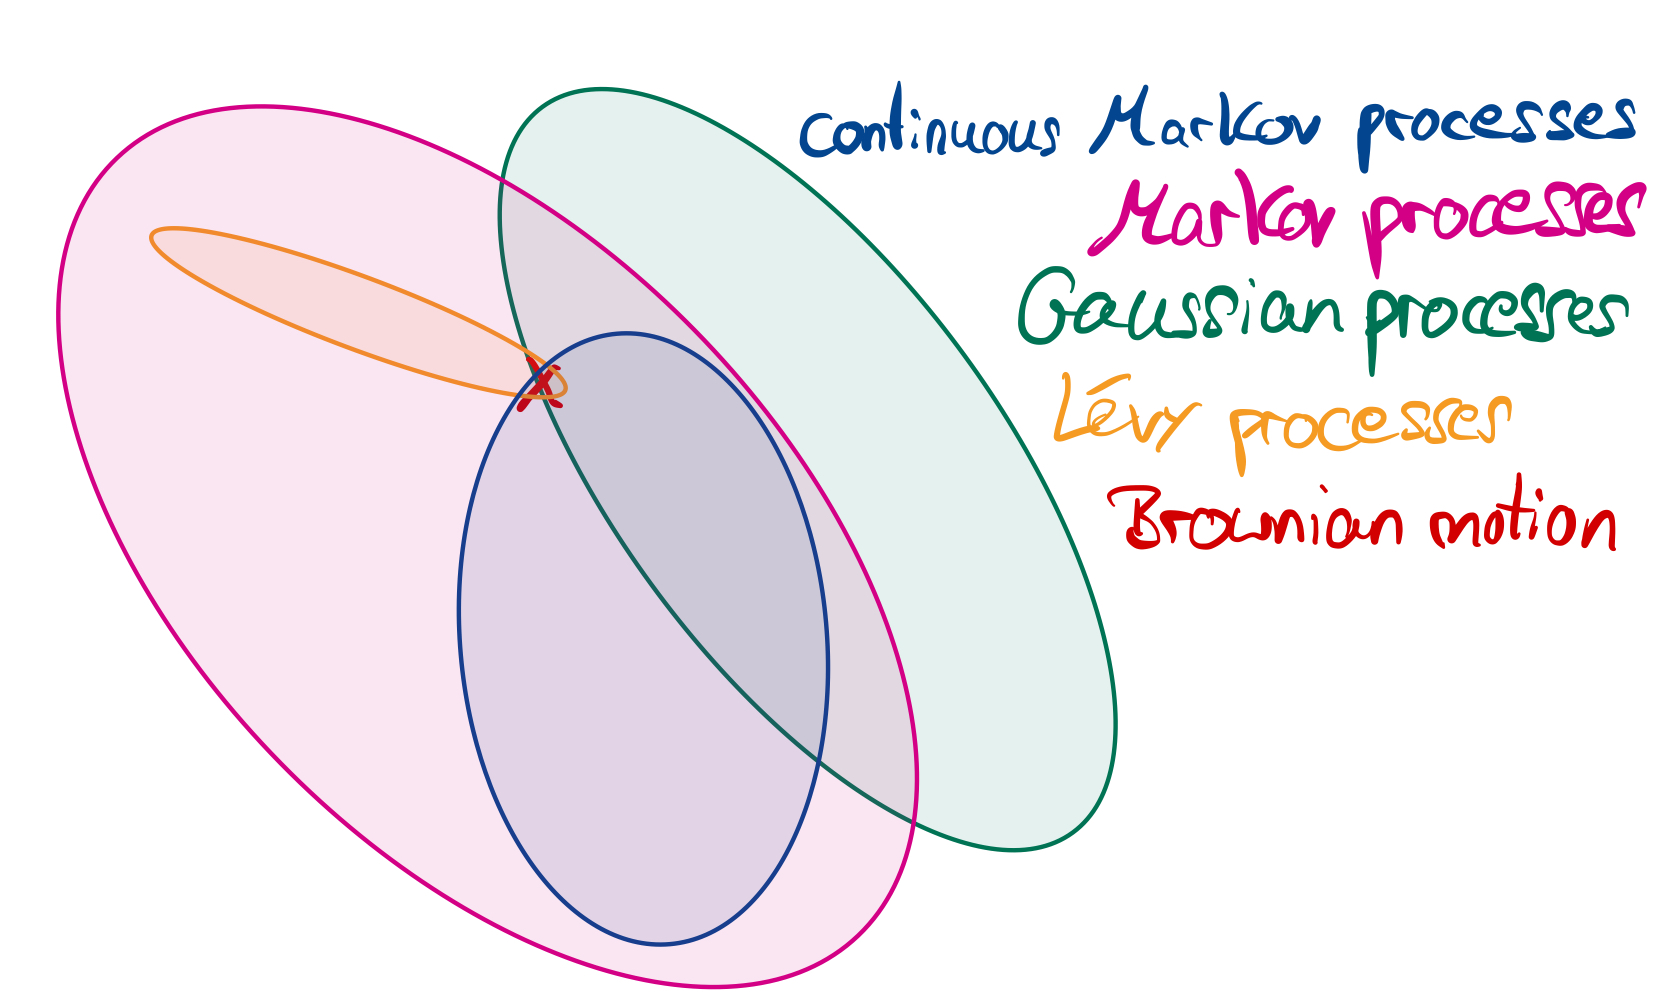
\includegraphics[scale=0.1]{processes.jpeg}
		\caption*{The most important classes of stochastic processes}
	\end{center}
\end{figure}
Along the example of the Brownian motion we will touch the most important classes of continuous-time stochastic processes: Markov processes, Gaussian processes, and L\'evy processes. We will start with a lengthy section on the measure theoretic foundations, then turn to Brownian motion and some of it's fascinating properties, and finally prove Donsker's theorem. Donsker's theorem shows that the Brownian motion is natural as a process in the sense that all second-moment discrete random-walks weakly converge to the Brownian motion if space and time are scaled appropriately.
\section[Stochastic processes in continuous time]{Introduction to stochastic processes in continuous time}\label{sec:SP}
	Let us first recall the definition of a stochastic process. For a fixed probability space $(\Omega, A, \P)$ a collection $X=(X_i)_{i\in I}$ of random variables with values in a measurable space $(E,\mathcal E)$ is called a stochastic process with state-space $E$. The visualizations of this chapter will always refer to $I=[0,\infty)$ so we will always use $t$ instead of $i$ and think of time even though the index set might be $I=\R^d$ and refer to space. For almost all examples of interest one can assume $E$ is a Polish metric space with Borel $\sigma$-algebra $\mathcal E=\mathcal B(E)$ but always keep in mind the most important example $E=\R$. The index set $I$ was assumed to be discrete in the discussion of martingales but can also be continuous here. The (random) mapping $t\mapsto X_t(\omega)$ is called a trajectory (or sample path) of $X$. While the study of discrete time stochastic processes was rather elementary (playing with stopping times and the martingale property) the study of continuous time processes will be more involved caused by the measure theory on path-space where the continuum appears twice (in space and time). An illustrative task is to answer (and properly define) the question if sample paths of stochastic processes are almost surely continuous or differentiable.\smallskip
	
In order to develop the full theory of stochastic processes we will first extend the triology of measure theory behind random vectors, i.e. stochastic processes with $|I|<\infty$, from Section \ref{sec:RV}:
\begin{itemize}
	\item define a $\sigma$-algebra $\mathcal E^{\otimes I}$ on the generic path space $E^I=\{f:I\to E\}$,
	\item understand all probability measures on $\mathcal E^{\otimes I}$,
	\item reinterprete stochastic processes as path-valued random variables.
\end{itemize}
There is quite a bit of pain involved in generalizations from finite $I$ to uncountable $I$ and even worse if trajectories $t\mapsto X_t(\omega)$ are supposed to be continuous, a topic we discuss a bit later.

\subsection{Stochastic processes and the generic path space}
The biggest hurdle towards a thorough understanding of continuous-time stochastic processes is the measure theory on path space. Even though the main interest of this course is processes with continuous sample paths (such as the Brownian motion) it is useful to first discuss measure theory on generic functions $f:I\to E$. With generic we mean functions with absolutely no assumptions, in contrast for instance to continuous functions. In the previous chapter we enlarged $[0,\infty)$ to the one-point compactification $[0,\infty]$ in order to gain compactness. It is much less simple to see what is gained if continuous functions $C([0,\infty))$ are enlarged to all generic functions $\R^{[0,\infty)}$. There is only one very non-trivial reason, the Kolmogorov extension theorem that we prove below. Kolmogorov's extension theorem is a tool that allows to construct measures on the natural $\sigma$-algebra on paths $\R^{\otimes [0,\infty)}$ which combined with the Kolmogorov-Chentsov theorem gives a possibility to construct measures on $C([0,\infty))$ and continuous-times stochastic processes. In order to bypass that hurdle we carefully discuss all appearing objects and new ideas, and then pass on to the Brownian motion as an application of the strategy. \smallskip




Before getting started it is useful to visualize and reinterpret the generic path space $\R^I$ of all functions from $I$ to $\R$ for the simplest index sets:
\begin{itemize}
	\item $\R^I$ corresponds to $\R$ if $|I|=1$,
	\item $\R^I$ corresponds to $\R^d$ if $|I|=d$, by reinterpreting a vector as a mapping from $d$ arbitrary time-points (the indices of the vector) to $\R$,
	\item $\R^I$ corresponds to the set of real-valued sequences for $I=\N$,
\end{itemize}

\begin{figure}[h]
	\begin{center}
	\begin{tikzpicture}[scale=0.6,transform shape]
			\tikzset{
			  pics/tick/.style args={#1}{code={
				\draw[line width=0.3mm,inner sep=0mm] (0,-#1) -- (0,#1) ;
				},
			  }
			}
			  \tikzset{
				cross/.pic ={
				  \draw[pic actions,rotate=#1,line width=0.3mm]
					(-3.5pt,0) -- (3.5pt,0)
					(0,-3.5pt) -- (0,3.5pt);
				},
			  }
			\draw[black!90,line width=0.3mm] (0,-1) -- ++(90:3cm);
			%AXIS X
			\draw[black!90,line width=0.3mm] (0,0) --++(0:3.5cm); 
			\draw (1,0) pic[rotate=0] {tick={1mm}} node[yshift=-2.5mm,xshift=2mm,scale=1.2] {$t_1$} ;
			\draw[darkgreen] (1,-0.5) pic {cross={45}} ;
			\draw[orange] (1,0.5) pic {cross={45}} ;
			\draw[red] (1,1.5) pic {cross={45}} ;
		\end{tikzpicture}
		\hspace{3mm}
		\begin{tikzpicture}[scale=0.6,transform shape]
			\tikzset{
			  pics/tick/.style args={#1}{code={
				\draw[line width=0.3mm,inner sep=0mm] (0,-#1) -- (0,#1) ;
				},
			  }
			}
			  \tikzset{
				cross/.pic ={
				  \draw[pic actions,rotate=#1,line width=0.3mm]
					(-3.5pt,0) -- (3.5pt,0)
					(0,-3.5pt) -- (0,3.5pt);
				},
			  }
			\draw[black!90,line width=0.3mm] (0,-1) -- ++(90:3cm);
			%AXIS X
			\draw[black!90,line width=0.3mm] (0,0) --++(0:5.5cm); 
			\draw (1,0) pic[rotate=0] {tick={1mm}} node[yshift=-2.5mm,xshift=2mm,scale=1.2] {$t_1$} ;
			\draw (2,0) pic[rotate=0] {tick={1mm}} node[yshift=-2.5mm,xshift=2mm,scale=1.2] {$t_2$} ;
			\draw (3,0) pic[rotate=0] {tick={1mm}} node[yshift=-2.5mm,xshift=2mm,scale=1.2] {$t_3$} ;
			%t1
			\draw[darkgreen] (1,-0.5) pic {cross={45}} ;
			\draw[orange] (1,0.5) pic {cross={45}} ;
			\draw[red] (1,1.5) pic {cross={45}} ;
			%t2
			\draw[darkgreen] (2,0.5) pic {cross={45}} ;
			\draw[orange] (2,1) pic {cross={45}} ;
			\draw[red] (2,1.5) pic {cross={45}} ;
			%t1
			\draw[darkgreen] (3,1) pic {cross={45}} ;
			\draw[orange] (3,1.5) pic {cross={45}} ;
			\draw[red] (3,2) pic {cross={45}} ;
		\end{tikzpicture}
		\hspace{3mm}
		\begin{tikzpicture}[scale=0.6,transform shape]
			\tikzset{
			  pics/tick/.style args={#1}{code={
				\draw[line width=0.3mm,inner sep=0mm] (0,-#1) -- (0,#1) ;
				},
			  }
			}
			  \tikzset{
				cross/.pic ={
				  \draw[pic actions,rotate=#1,line width=0.3mm]
					(-3.5pt,0) -- (3.5pt,0)
					(0,-3.5pt) -- (0,3.5pt);
				},
			  }
			\draw[black!90,line width=0.3mm] (0,-1) -- ++(90:3cm);
			%AXIS X
			\draw[black!90,line width=0.3mm] (0,0) --++(0:4.5cm); 
			\draw (1,0) pic[rotate=0] {tick={1mm}} node[yshift=-2.5mm,xshift=2mm,scale=1.2] {1} ;
			\draw (2,0) pic[rotate=0] {tick={1mm}} node[yshift=-2.5mm,xshift=2mm,scale=1.2] {2} ;
			\draw (3,0) pic[rotate=0] {tick={1mm}} node[yshift=-2.5mm,xshift=2mm,scale=1.2] {3} ;
			\draw (4,0) pic[rotate=0] {tick={1mm}} node[yshift=-2.5mm,xshift=2mm,scale=1.2] {4} ;
			%\draw (5,0) pic[rotate=0] {tick={1mm}} node[yshift=-2.5mm,xshift=2mm,scale=1.2] {5} ;
			%0
			\draw[darkgreen] (0,0.9) pic {cross={45}} ;
			\draw[orange] (0,0.4) pic {cross={45}} ;
			\draw[red] (0,1.5) pic {cross={45}} ;
			%1
			\draw[darkgreen] (1,0.5) pic {cross={45}} ;
			\draw[orange] (1,1.5) pic {cross={45}} ;
			\draw[red] (1,1) pic {cross={45}} ;
			%2
			\draw[darkgreen] (2,-0.5) pic {cross={45}} ;
			\draw[orange] (2,1.5) pic {cross={45}} ;
			\draw[red] (2,1) pic {cross={45}} ;
			%3
			\draw[darkgreen] (3,0.25) pic {cross={45}} ;
			\draw[orange] (3,0.75) pic {cross={45}} ;
			\draw[red] (3,1.25) pic {cross={45}} ;
			%4
			\draw[darkgreen] (4,0.5) pic {cross={45}} ;
			\draw[orange] (4,1) pic {cross={45}} ;
			\draw[red] (4,1.5) pic {cross={45}} ;
			%5
			%\draw[darkgreen] (5,0.5) pic {cross={45}} ;
			%\draw[orange] (5,1) pic {cross={45}} ;
			%\draw[red] (5,1.5) pic {cross={45}} ;
		\end{tikzpicture}
		\caption*{A few elements of $\R^{\{t_1\}}$, $\R^{\{t_1,t_2,t_3\}}$, and $\R^{\N}$.}
	\end{center}
\end{figure}
The target will always be to generalize ideas from $\R^d$ to $\R^I$ by keeping the illustrations in mind. Before starting the measure theory on path space the reader might want to have a quick look at Section \ref{sec:ZV} to recall the trilogy of steps $\sigma$-algebra, measures, random variables for $\R^d$ as the next sections are similar but more delicate in terms of notation.

\subsubsection{(A) The path $\sigma$-algebra}
Recall from Section \ref{sec:Fubini} the notion of a product $\sigma$-algebra. If $\mathcal E$ is a $\sigma$-algebra, then the $d$-fold product $\sigma$-algebra on $E^d$ is defined as 
\begin{align*}
	\mathcal E^{\otimes d}:=\mathcal E\otimes \cdots \otimes \mathcal E:=\sigma(\{B_1\times \cdots \times B_d: B_i\in \mathcal E\}).
\end{align*}
In the sequel the appearing sets $B_1\times \cdots \times B_d$ are called \textbf{boxes} and interpreted using the reinterpretation of $E^d$ as mappings from $d$ arbitrary time-points to $E$. If $\mathcal E=\sigma(\mathcal A)$, then $\mathcal E^{\otimes d}$ can also be expressed as
\begin{align*}
	\mathcal E^{\otimes d}=\sigma(\{B_1\times \cdots \times B_d: B_i\in \mathcal A\}).
\end{align*}
Most importantly, if $E=\R$ and $\mathcal A$ is chosen as the set of intervals than the product $\sigma$-algebra is generated by rectangular boxes.
\begin{figure}[h]
	\begin{center}
    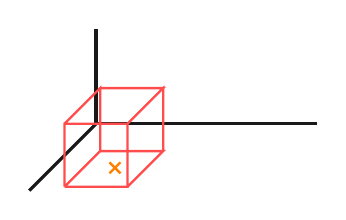
\begin{tikzpicture}[scale=0.8,transform shape]
	\tikzset{
	  pics/tick/.style args={#1}{code={
		\draw[line width=0.3mm,inner sep=0mm] (0,-#1) -- (0,#1) ;
		},
	  }
	}

          \tikzset{
            cube/.pic ={
              \draw[pic actions,line width=0.3mm]
         (0,0) -- ++(0:1cm) -- ++(45:0.8cm) -- ++(0:-1cm) -- ++(45:-0.8cm)
        (0,0) -- ++(0:1cm) -- ++(45:0.8cm) -- ++(0:-1cm) -- ++(45:-0.8cm)
        (0,0) -- ++(90:1cm) --++(45:0.8cm) -- ++(90:-1cm)
        (0,0) -- ++(0:1cm) -- ++(90:1cm) -- ++(45:0.8cm) -- ++(90:-1cm)
        (0,0) -- ++(90:1cm) --++(0:1cm) -- ++(45:0.8cm) --++(0:-1cm);
            }
          }
        \tikzset{
            cross/.pic ={
              \draw[pic actions,rotate=#1,line width=0.3mm]
                (-3.5pt,0) -- (3.5pt,0)
                (0,-3.5pt) -- (0,3.5pt);
            },
          }


        %AXIS Y
        \draw[black!90,line width=0.4mm] (0,0) -- ++(90:1.5cm);
        %AXIS X
        \draw[black!90,line width=0.4mm] (0,0) --++(0:3.5cm);  
        %AXIS Z 
        \draw[black!90,line width=0.4mm] (0,0) --++(45:-1.5cm);  

        %cube 
        \draw[red!70] (-0.5,-1) pic {cube} ;
        \draw[orange] (0.3,-0.7) pic {cross={45}};
     %   \draw[darkgreen] (0.2,0.2) pic {cross={45}}; 
    \end{tikzpicture} 
    \hspace{5mm}
    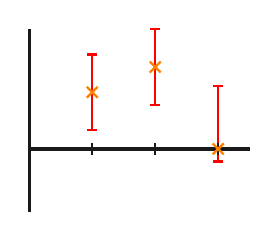
\begin{tikzpicture}[scale=0.8,transform shape]
        \tikzset{
          pics/tick/.style args={#1}{code={
            \draw[line width=0.3mm,inner sep=0mm] (0,-#1) -- (0,#1) ;
            },
          }
        }
        \tikzset{
            cross/.pic ={
              \draw[pic actions,rotate=#1,line width=0.3mm]
                (-3.5pt,0) -- (3.5pt,0)
                (0,-3.5pt) -- (0,3.5pt);
            },
          }
		  \tikzset{
pics/intervall/.style args={#1}{code={
\draw[red,line width=0.3mm] (0,0) -- ++(0,#1) 
node[rotate=90,sloped,inner xsep=0.8mm,inner ysep=0,pos=1,fill,red] (E) {}
node[rotate=90,sloped,inner xsep=0.8mm,inner ysep=0,pos=0,fill,red] (E) {};
},
}
}
\draw  (1,0.3)  pic {intervall={1.2}} ;
\draw  (2,0.7)  pic {intervall={1.2}};
\draw  (3,-0.2)  pic {intervall={1.2}} ;
		  
        %AXIS Y
        \draw[black!90,line width=0.4mm] (0,-1) -- ++(90:2.9cm);
        %AXIS X
        \draw[black!90,line width=0.4mm] (0,0) --++(0:3.5cm);  
        \draw[black!90] (1,0) pic {tick={1mm}};
        \draw[black!90] (2,0) pic {tick={1mm}};
        \draw[black!90] (3,0) pic {tick={1mm}};
       
      %  \draw[darkgreen] (1,1) pic {cross={45}};
        \draw[orange] (1,0.9) pic {cross={45}};
        %\draw[red,line width=0.3mm] (1,0.3) -- ++(90:12mm);

        %\draw[red,line width=0.3mm] (2,0.7) -- ++(90:12mm);
        %\draw[darkgreen] (2,0.8) pic {cross={45}};
        \draw[orange] (2,1.3) pic {cross={45}};

        %\draw[red,line width=0.3mm] (3,0) -- ++(90:12mm);
        %\draw[darkgreen] (3,1) pic {cross={45}};
        \draw[orange] (3,0) pic {cross={45}};
    \end{tikzpicture}
	\caption*{Reinterpretation of a three-dimensional rectengular box for arbitrary three time-pointes}
\end{center}
\end{figure}


The aim is to introduce a generalization to infinite products, but what is a good notion for a (possibly uncountable) infinite product of sets?
As usually in Mathematics the trick is to reduce as far as possible to the finite case:
\begin{ldef}
	\begin{deff}
		A subset $C$ of $E^I$ is called \textbf{finitely generated cylinder set} if 
		\begin{align*}
			C&=\pi_{J}^{-1}(B_1\times \cdots \times B_n)\\
			&=\{f:I\to E\,|\, f(t_1)\in B_1, ..., f(t_n)\in B_n\},
		\end{align*}
		where $J=\{t_1,...,t_n\}\subseteq I$ and $B_1,...,B_n\in \mathcal E$. The projections $\pi_J:E^I\to E^{|J|}$,  $$\pi_{J}(f)=(f(t_1),...,f(t_n)),$$ evaluate a path at finitely many given time-points. We also say the set $C$ of paths is spanned by the finitely many time-points $t_1,...,t_d$ and the finite-dimensional box $B_1\times \cdots \times B_d \in \mathcal E^{\otimes n}$.	
		%To abbreviate we also write $C_J^B$ for the finite subset $J=\{t_1,...,t_n\}$ of $I$ and $B=B_1\times \cdots B_n$.
	\end{deff}
\end{ldef}
Some of the $B_i$ will typically be equal to $E$, not imposing a restriction. Before proceeding it is extremely important to gain a visual understanding of  finitely generated cylinder sets. The picture to keep in mind is that of a box tied to the time-points with all possible functions $I\to E$ passing through the box, the cylinder set of functions consists of all the functions passing through the box. 
\begin{figure}[h]
\begin{center}
	\begin{tikzpicture}
	\tikzset{
	  pics/tick/.style args={#1}{code={
		\draw[line width=0.3mm,inner sep=0mm] (0,-#1) -- (0,#1) ;
		},
	  }
	}
\tikzset{
pics/intervall/.style args={#1}{code={
\draw[red,line width=0.3mm] (0,0) -- ++(0,#1) 
node[rotate=90,sloped,inner xsep=0.8mm,inner ysep=0,pos=1,fill,red] (E) {}
node[rotate=90,sloped,inner xsep=0.8mm,inner ysep=0,pos=0,fill,red] (E) {};
},
}
}
	%AXIS Y
	\draw[black!90,line width=0.4mm] (0,-0.6) -- ++(90:2.5cm);
	%AXIS X
	\draw[black!90,line width=0.4mm] (0,0) --++(0:3.5cm);  
	\draw (1,0) pic[rotate=0] {tick={1mm}} node[yshift=-2.5mm,xshift=2mm,scale=1.2] {$t_1$} ;
	\draw (2,0) pic[rotate=0] {tick={1mm}} node[yshift=-2.5mm,xshift=2mm,scale=1.2] {$t_2$} ;
	\draw (3,0) pic[rotate=0] {tick={1mm}} node[yshift=-2.5mm,xshift=2mm,scale=1.2] {$t_3$} ;

  \draw  (1,0.5)  pic {intervall={0.6}} ;
  \draw  (2,0.5)  pic {intervall={0.6}};
  \draw  (3,0.1)  pic {intervall={0.6}} ;
	
  %func 1 
  \draw[orange,line width=0.3mm] (0,0.5) .. controls (1.5,1.5) and  (2,0.4) .. (2.5,0.8);
  \draw[orange,line width=0.3mm] (2.5,0.4) .. controls (3,0)  .. (3.5,0.8);

  %func 2
  \draw[blue,line width=0.3mm] (0,1.5) .. controls (1,0.5) .. (1.8,0.8);
  \draw[blue,line width=0.3mm] (1.8,0.9) .. controls (2,0.8)  .. (2.5,1.1);
  \draw[blue,line width=0.3mm] (2.5,1.3) .. controls (3,0.1)  .. (3.5,0.3);

  %func 3
  \draw[darkgreen,line width=0.3mm] (0,1) .. controls (1,0.5) and (2,1.3) .. (3.5,0.2);
\end{tikzpicture} 
\caption*{A cylinder set is a set functions passing through the given box tied at given times}
\end{center}
\end{figure}
There are two quantities that have to be distinguished very carefully. The spanning box, which is a finite-dimensional measurable set, and the cylinder set which is a set of functions. 
\begin{ldef}
\begin{deff}
		 The \textbf{path $\sigma$-algebra} (or \textbf{product $\sigma$-algebra}) $\mathcal E^{\otimes I}$ on $E^I$ is the smallest $\sigma$-algebra that contains all finitely generated cylinder sets.
		In the special case $(\R,\mathcal B(\R))$ one typically writes $\mathcal B(\R^d)$, $\mathcal B(\R^\infty)$, $\mathcal B(\R^{[0,T]})$ to keep the notation short.
	\end{deff}
\end{ldef}
To get an idea of the definition it is useful to compare the cases $|I|=d$ and $I=\N$ for $E=\R$. For the first the cylinder sets are just boxes. The path $\sigma$-algebra is nothing but the well-known $d$-fold product $\mathcal B(\R^d)=\mathcal B(\R)^{\otimes d}$ from Section \ref{sec:ZV}. This motivates why the path $\sigma$-algebras is also called product $\sigma$-algebra for infinite index sets. The infinite product structure becomes more visible for $I=\N$, where the finitely generated cylinder sets are actually infinite products of the type $\R\times B_1 \times \cdots \times B_2\times \R \times \cdots$ where only the finitely many factors impose a restriction. While the infinite cartesian product makes sense for sequences the good way of writing an uncountable product with restrictions at finitely many time-points is the formalism using projections $\pi_J$ on finitely many time-points.\smallskip


Here are two simple exercise that we will later need and that is very useful to get acquainted with the new definitions.
\begin{luebung}
	Show that the set of all finitely generated cylinder sets form a semiring. First draw some pictures and then try to formalize your findings using projections.
\end{luebung}



As always there are many different generators of the $\sigma$-algebra, not all are equally useful.
\begin{luebung}
	Suppose that $\mathcal E=\sigma(\mathcal A)$. Check that 
	\begin{align*}
		\mathcal E^{\otimes I}&= \sigma( \{\pi^{-1}_{t_1,...,t_n}(B_1\times \cdots \times B_n):n\in\N, t_i\in J, B_i\in \mathcal A\}),\\
		\mathcal E^{\otimes I}&= \sigma( \{\pi_i^{-1}(B):i \in I, B\in  \mathcal E \}),\\	
		\mathcal E^{\otimes I}&= \sigma( \{\pi_i^{-1}(B):i \in I, B\in  \mathcal A\})
	\end{align*}
	and draw some examples of sets of paths in the generators of $\mathcal E^{\otimes I}$.	Which of the generators of $\mathcal E^{\otimes I}$ is intersection stable?
\end{luebung}
If $|I|<\infty$ or $I$ is countable not much more needs to be said, there are no bad surprises, everything works more or less similarly to $\mathcal B(\R^d)$. The only trouble is the usual difference between $\mathcal P(\R^d)$ and $\mathcal B(\R^d)$ that arises from the fact that countable set operations in a $\sigma$-algebra do not allow to approximate arbitrary subsets from $\R^d$ using intervals/open sets/closed sets/etc. Most interesting sets of interest belong to $\mathcal B(\R^d)$, the generator is rich enough. The story is very different for uncountable index sets $I$ because a second and more severe uncountability issue appears. The generator of $\mathcal E^{\otimes I}$ only uses single (or finitely many) points in time which is by far not enough to capture a lot of information about functions in time. It is instructive to compare with Example \ref{bspd} where it was shown that the smallest $\sigma$-algebra containing singletons can only cover the countable sets and their complements. Hence, a $\sigma$-algebra defined using finitely generated cylinder sets only can at most cover countably many restrictions. To make this formal we call a set finitely generated if there is a countable set (i.e. finite or countably infinite) $J\subseteq I$ of time-points such that
\begin{align*}
	f\in C\quad \Leftrightarrow \quad f_{|J}\in B
\end{align*}
for some $B\in \mathcal E^{\otimes J}$. In words, a countably generated set is a set of functions that has only restrictions at countably many time-points. Note that here we do not only use boxes $B_1\times \cdots \times B_d$, we speak of countably generated sets in contrast to countably generated cylinder sets. The reason is the next proposition, only cylinder sets are not enough to form a $\sigma$-algebra. Think for instance of $\R^2$ where only the rectangles do not form a $\sigma$-algebra as for instance circles belong to $\mathcal B(\R^2)$.
\begin{laussagewerkzeug}
\begin{prop}
	The set $\mathcal V$ of all \underline{countably} generated sets is a $\sigma$-algebra on $E^I$ that contains $\mathcal E^{\otimes I}$.%, where a set $A\subseteq E^I$ is called countably generated if there is a countable subset $J\subseteq I$ and a set $B\in \mathcal E^J$ such that 
	%\begin{align*}
	%	f\in A\quad \Leftrightarrow \quad f_{|J}\in B.
	%\end{align*}
\end{prop}
\end{laussagewerkzeug}
\begin{proof}[Proof]
	To check the three properties of a $\sigma$-algebra is straight forward:\smallskip

	(i) Choosing $J$ to be an arbitrary singleton and $B=E$ proves that $\Omega=E^I$ is countably generated.\smallskip
	
	(ii) If $C$ is spanned by a countable set $J=\{t_1,...\}$ and $B\in \mathcal E^{\otimes J}$, then $C^c$ is spanned by the same set $J$ and the measurable set $B^c\in \mathcal E^{\otimes J}$, so $C^c$ is again countably generated.
	\begin{luebung}
		(iii) Check that $\mathcal V$ is closed under taking countable unions. First draw a picture to understand what is going on, then formalize your picture.
	\end{luebung}
	Since all finitely generated cylinder sets are also infinitely generated sets, the generator of $\mathcal E^{\otimes I}$ is a subset of $\mathcal V$. Hence, $\mathcal E^{\otimes I}\subseteq \sigma(\mathcal V)=\mathcal V$ which is the claim.
\end{proof}
The proposition has dramatic consequences! Almost all sets of paths that one might be interested in to study the behavior of paths $t\mapsto X_t(\omega)$ are \textbf{not measurable} in the product $\sigma$-algebra on paths!
\begin{example}
	Suppose $E=\R$ and $I=\R$, $I=[0,1]$, or $I=[0,\infty)$. 
	\begin{itemize}
	\item Singleton sets $\{f\}$ containing only a single path are not measurable.
	\item The set of all constant functions $\{f\equiv c\,|\,c\in E\}$ is not measurable.
	\item The set of all non-negative functions $\{ f:I\to E\,|\, f\geq 0\}$ is not measurable.
	\item The set of all continuous functions $\{f:I\to E\,|\, f\text{ continuous}\}$ is not measurable.
	\item  The set of all differentiable functions $\{f:I\to E\,|\, f\text{ differentiable}\}$ is not measurable.
	\end{itemize}
\end{example}
The reason is simple. If any of those sets was measurable in the $\sigma$-algebra $\R^{\otimes I}$ of paths, then there should be a countable set $J$ of time-points that spans the set. If $I$ is uncountable there is an index $i\notin J$. Now take a function $f$ from the sets and add some value at $i$ that destroys the defining property. Then the new function $\tilde f$ is still in the set as the values on $J$ are not changed. But then the set contains a function that violates the defining property which should not be the case. As a consequence we should be very careful with statements of the kind "{}$\P$-almost all paths are continuous"{} for measures on the uncountable product $\sigma$-algebras on paths. There is actually a fun point about this observation. Whereas it is very non-trivial to find sets which are not Borel-measurable in $\R$ it is the typical case that sets are not measurable in $\mathcal B(\R^{[0,\infty)})$. The reason is just that time and space are treated very differently in the definition of cylinder sets (finite sets vs. Borel-sets).\smallskip

Since uncountable product $\sigma$-algebras are delicate one should ask if the decision to work with $\mathcal E^{\otimes I}$ was clever or non-sense. The surprising answer is clever as there is a natural way to construct measures on $\mathcal E^{\otimes I}$ and most delicate issues about zero sets and path properties can be resolved.
\marginpar{\textcolor{red}{Lecture 20}}

\subsubsection{(B) Probability measures on paths}
The aim of this section is to identify all probability measures on the product $\sigma$-algebra $\mathcal E^{\otimes I}$. For $E=\R$ and $|I|<\infty$ this has already been done in Section \ref{sec:VF}, we now generalize to arbitrary $I$ and $E$ as long as $E$ is a Polish space. The strategy is not simple but can be compared to the theory of distribution functions for probability measures on $\mathcal B(\R)$. Recall the approach from Section \ref{sec:VF}:
\begin{enumerate}[label=(\roman*)]
	\item Downsize the information of a measure into something simple that uniquely characterizes the measure (some $\cap$-stable generator). In that case the simplest $\cap$-stable generator of $\mathcal B(\R)$ was the set of all intervals and we defined $F(t)=\P((-\infty,t])$, $t\in\R$.
	\item Identify natural properties of the simpler object. We used continuity of measures to deduce monotonicity, limits at infinity, and right-continuity for $F$. Such functions were then called distribution functions.
	\item Reverse the game: Show that for all distribution function there is a corresponding probability measure (Carath\'eodory extension theorem)
\end{enumerate}
The approach for measures on $\mathcal E^{\otimes I}$ is exactly the same:
\begin{enumerate}[label=(\roman*)]
	\item Downsized $\P$ by only considering events from the finite cylinder sets (which are $\cap$-stable). This leads to so-called finite-dimensional distributions $\P_J$ on $\mathcal E^{\otimes J}$ for all finite subsets $J\subseteq I$.
	\item Check that the family $\{\P_J: |J|<\infty\}$ of all finite-dimensional distributions satisfies a natural property, consistency.
	\item Reverse the game: Show that for all consistent families of finite-dimensional distributions there is a corresponding probability measures (Carath\'eodory consistency theorem).
\end{enumerate}
The only trouble of the approach comes from the notation. The notation with cylinder sets and finite-dimensional distributions is either very long (writing out all appearing cylinder sets) or very compact (using projections). We will stick to the compact way combined with many illustrations.\smallskip

Here is the first step, the restrictions to the $\cap$-stable generator of finitely generated cylinder sets.
\begin{ldef}
\begin{deff}\label{def:SL}
	If $\P$ is a probability measure on $\mathcal E^{\otimes I}$ and $J\subseteq I$ is finite, then the unique measure on $\mathcal E^{\otimes J}$ defined by
	\begin{align*}
		\P_J(B_1\times \cdots \times B_{|J|}):=\P(\pi_{J}^{-1}((B_1\times \cdots \times B_{|J|})),\quad B_i\in \mathcal E,
	\end{align*}
	is called a \textbf{finite-dimensional marginal distribution} of $\P$.
\end{deff}
\end{ldef}
Here is a very important point to understand. On the one hand we have boxes (measurable sets of a finite-dimensional space) on the other hand we have cylinder sets of functions passing through the boxes at time-points $J$ (measurable sets of an infinite-dimensional space). The finite-dimensional marginals are the measures that we get by crossing out the functions away from $J$.

\begin{figure}[h]
	\begin{center}
    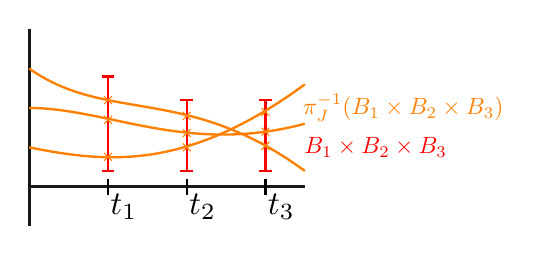
\begin{tikzpicture}
    \tikzset{
      pics/cross/.style args={#1,#2}{code={
      \draw[rotate=#1] (-#2pt,0) -- (#2pt,0)
        (0,-#2pt) -- (0,#2pt);
      },
    }
    }
    \tikzset{
      pics/tick/.style args={#1}{code={
        \draw[line width=0.3mm,inner sep=0mm] (0,-#1) -- (0,#1) ;
        },
      }
    }
\tikzset{
  pics/intervall/.style args={#1}{code={
    \draw[red,line width=0.3mm] (0,0) -- ++(0,#1) 
    node[rotate=90,sloped,inner xsep=0.8mm,inner ysep=0,pos=1,fill,red] (E) {}
    node[rotate=90,sloped,inner xsep=0.8mm,inner ysep=0,pos=0,fill,red] (E) {};
  },
}
}
        %AXIS Y
        \draw[black!90,line width=0.4mm] (0,-0.5) -- ++(90:2.5cm);
        %AXIS X
        \draw[black!90,line width=0.4mm] (0,0) --++(0:3.5cm);   

        \draw (1,0) pic[rotate=0] {tick={1mm}} node[yshift=-2.5mm,xshift=2mm,scale=1.2] {$t_1$} ;
        \draw (2,0) pic[rotate=0] {tick={1mm}} node[yshift=-2.5mm,xshift=2mm,scale=1.2] {$t_2$} ;
        \draw (3,0) pic[rotate=0] {tick={1mm}} node[yshift=-2.5mm,xshift=2mm,scale=1.2] {$t_3$} ;

      \draw  (1,0.2)  pic {intervall={1.2}} ;
      \draw  (2,0.2)  pic {intervall={0.9}};
      \draw  (3,0.2)  pic {intervall={0.9}} ;

      \draw[orange] (1,0.38) pic {cross={45,2}};
      \draw[orange] (1,0.85) pic {cross={45,2}};
      \draw[orange] (1,1.1) pic {cross={45,2}};

      \draw[orange] (2,0.5) pic {cross={45,2}};
      \draw[orange] (2,0.9) pic {cross={45,2}};
      \draw[orange] (2,0.68) pic {cross={45,2}};

      \draw[orange] (3,0.7) pic {cross={45,2}};
      \draw[orange] (3,0.95) pic {cross={45,2}};
      \draw[orange] (3,0.52) pic {cross={45,2}};
        
      \draw[orange,line width=0.3mm] (0,0.5) .. controls (1,0.3) and  (2,0.2) .. (3.5,1.3);
      \draw[orange,line width=0.3mm] (0,1) .. controls (1,1) and  (2,0.4) .. (3.5,0.8);
      \draw[orange,line width=0.3mm] (0,1.5) .. controls (1,0.8) and  (2,1.3) .. (3.5,0.2);

    % \draw[red] (0.5,1) pic {cross={45,8}};
    %\draw[black,line width=0.2mm] (0.2,0.3) -- ++(65:1.2cm);
    %\draw[black,line width=0.2mm] (0.2,1.5) -- ++(-65:1.35cm);
%
 %   \draw[black,line width=0.2mm] (1.3,0.3) -- ++(65:1cm);
  %  \draw[black,line width=0.2mm] (1.3,1.2) -- ++(-65:1cm);
%
 %   \draw[black,line width=0.2mm] (2.3,0.3) -- ++(65:0.8cm);
  %  \draw[black,line width=0.2mm] (2.3,1) -- ++(-65:0.8cm);


    \node[orange,scale=0.85] (pi) at (4.6,1) {$\quad\pi_{J}^{-1}(B_1\times B_2\times B_3)$} ;
    \node[red,scale=0.85] (B) at (4.25,0.5) {$\quad B_1\times B_2\times B_3$} ;
    \end{tikzpicture} 
  \caption*{Restricting the functions at J = $\{t_1,t_2,t_3\}$ to $B_1\times B_2\times B_3$ }
\end{center}
\end{figure}

The set of finite-dimensional marginals $\P_J$ is much easier than $\P$ as these are only measures on finite product $\sigma$-algebras $\mathcal E^{\otimes J}$ that only need to be defined on rectangular $B_1\times \cdots\times B_d$ and can be uniquely extended to a measure using Carath\'eodory's extension theorem (see Theorem \ref{Car2} for $\mathcal B(\R^d)$). This reflects the analogy that distribution functions are much simpler than probability measures on $\mathcal B(\R)$. Similarly to distribution functions of measures on $\mathcal B(\R)$ the finite-dimensional distributions uniquely define $\P$:
\begin{laussagewerkzeug}\label{lemma:unique}
\begin{prop}
	Every probability measure $\P$ on $\mathcal E^{\otimes I}$ is uniquely defined through the family of all finite-dimensional marginal distributions $\{\P_J:|J|<\infty\}$.
\end{prop}
\end{laussagewerkzeug}
\begin{proof}[Proof]
	By the uniqueness theorem \ref{Dynkin-Folgerung}, $\P$ is uniquely defined on any $\cap$-stable generator of the product $\sigma$-algebra $\mathcal E^{\otimes I}$. We chose the set of all finitely generated cylinder sets
	\begin{align*}
		\mathcal S:=\{\pi_J^{-1}(B_1\times \cdots \times B_{|J|}):J \subseteq I, |J|<\infty, B_i\in  \mathcal E\},
	\end{align*}
	which is a generator of $\mathcal E^{\otimes I}$ and clearly intersection stable because the intersection of two boxes is a box. Here it is crucial to use the finitely generated sets and not the sets generated by all single time-points as the latter is not $\cap$-stable!
\end{proof}
The next step in the analogy to distribution functions is to derive what will later turn out to be the right characterizing property of families of finite-dimensional distributions to be related to measures on $\mathcal E^{\otimes I}$. 
\begin{laussagewerkzeug}
	\begin{prop}
	If $\P$ is a probability measures on $\mathcal E^{\otimes I}$, then the family of all finite-dimensional marginal distributions $\{\P_J:|J|<\infty\}$ fulfills the following property. If $J\subseteq J'$ are both finite subsets of $I$ and $\pi_{J,J'}$ denotes the projection from $E^J$ to $E^{J'}$, i.e. $\pi_{J,J'}(f)=f_{|J'}$, then
		\begin{align*}
			\P_J \circ \pi^{-1}_{J,J'}=\P_{J'}.
		\end{align*}
	\end{prop}
\end{laussagewerkzeug}
The proof is simple, only the notation is troubling. The projection $\pi_{J,J'}$ has the following meaning. Take a function indexed by $J$ and ignore all values from $J\backslash J'$. More interestingly, the preimage under $\pi_{J,J'}$ of a box spanned by $J'$ is the box spanned by $J$ with $E$ placed at the missing time-points from $J\backslash J'$. Here is a drawing: 
\begin{figure}[h]
	\begin{center}
    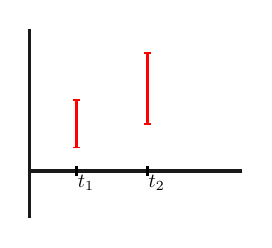
\begin{tikzpicture}[scale=0.6,transform shape]

\tikzset{
	pics/intervall/.style args={#1}{code={
	\draw[red,line width=0.3mm] (0,0) -- ++(0,#1) 
	node[rotate=90,sloped,inner xsep=0.8mm,inner ysep=0,pos=1,fill,red] (E) {}
	node[rotate=90,sloped,inner xsep=0.8mm,inner ysep=0,pos=0,fill,red] (E) {};
	},
	}
	}
        \tikzset{
          pics/tick/.style args={#1}{code={
            \draw[line width=0.3mm,inner sep=0mm] (0,-#1) -- (0,#1) ;
            },
          }
        }
          \tikzset{
            cross/.pic ={
              \draw[pic actions,rotate=#1,line width=0.3mm]
                (-3.5pt,0) -- (3.5pt,0)
                (0,-3.5pt) -- (0,3.5pt);
            },
          }
		  \draw  (1,0.5)  pic {intervall={1}} ;
		  \draw  (2.5,1)  pic {intervall={1.5}};

        \draw[black!90,line width=0.4mm] (0,-1) -- ++(90:4cm);
        %AXIS X
        \draw[black!90,line width=0.4mm] (0,0) --++(0:4.5cm); 
        \draw (1,0) pic[rotate=0] {tick={1mm}} node[yshift=-2.5mm,xshift=2mm,scale=1.2] {$t_1$} ;
        \draw (2.5,0) pic[rotate=0] {tick={1mm}} node[yshift=-2.5mm,xshift=2mm,scale=1.2] {$t_2$} ;
        %t1
        %\draw[red,line width=0.2mm] (1,0.5) -- (1,1.6);
        %\draw[orange] (1,1.5) pic {cross={45}} ;
        %\draw[blue] (1,0.5) pic {cross={45}} ;
        %t2
        %\draw[red,line width=0.2mm] (2,1) -- (2,1.6);
        %\draw[orange] (3,1) pic {cross={45}} ;
        %\draw[blue] (3,1.5) pic {cross={45}} ;
    \end{tikzpicture} 
    \hspace{5mm}
    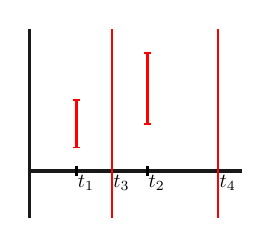
\begin{tikzpicture}[scale=0.6,transform shape]
		\tikzset{
	pics/intervall/.style args={#1}{code={
	\draw[red,line width=0.3mm] (0,0) -- ++(0,#1) 
	node[rotate=90,sloped,inner xsep=0.8mm,inner ysep=0,pos=1,fill,red] (E) {}
	node[rotate=90,sloped,inner xsep=0.8mm,inner ysep=0,pos=0,fill,red] (E) {};
	},
	}
	}
        \tikzset{
          pics/tick/.style args={#1}{code={
            \draw[line width=0.3mm,inner sep=0mm] (0,-#1) -- (0,#1) ;
            },
          }
        }
          \tikzset{
            cross/.pic ={
              \draw[pic actions,rotate=#1,line width=0.3mm]
                (-3.5pt,0) -- (3.5pt,0)
                (0,-3.5pt) -- (0,3.5pt);
            },
          }

		  \draw  (1,0.5)  pic {intervall={1}} ;
		  \draw  (2.5,1)  pic {intervall={1.5}};

        \draw[black!90,line width=0.4mm] (0,-1) -- ++(90:4cm);
        %AXIS X
        \draw[black!90,line width=0.4mm] (0,0) --++(0:4.5cm); 
        \draw (1,0) pic[rotate=0] {tick={1mm}} node[yshift=-2.5mm,xshift=2mm,scale=1.2] {$t_1$} ;
        \draw (2.5,0) pic[rotate=0] {tick={1mm}} node[yshift=-2.5mm,xshift=2mm,scale=1.2] {$t_2$} ;
        \draw (1.75,0) pic[rotate=0] {tick={1mm}} node[yshift=-2.5mm,xshift=2mm,scale=1.2] {$t_3$} ;
        \draw (4,0) pic[rotate=0] {tick={1mm}} node[yshift=-2.5mm,xshift=2mm,scale=1.2] {$t_4$} ;
        %t1
        %\draw[red,line width=0.2mm] (1,0.5) -- (1,1.6);
       % \draw[orange] (1,1.5) pic {cross={45}} ;
       % \draw[blue] (1,0.5) pic {cross={45}} ;
        %t2
        %\draw[red,line width=0.2mm] (2.5,1) -- (2.5,1.6);
       % \draw[orange] (2.5,1) pic {cross={45}} ;
        %\draw[blue] (2.5,1.5) pic {cross={45}} ;

        %t3
        \draw[red,line width=0.3mm] (1.75,-1) -- (1.75,3);
        %\draw[orange] (1.75,1.8) pic {cross={45}} ;
        %\draw[blue] (1.75,1) pic {cross={45}} ;

        %t4
        \draw[red,line width=0.3mm] (4,-1) -- (4,3);
        %\draw[orange] (4,1.8) pic {cross={45}} ;
        %\draw[blue] (4,1) pic {cross={45}} ;
    \end{tikzpicture} 
  \caption*{$B_1 \times B_2$ and $\pi_{J,J'}^{-1}(B_1 \times  B_2)$ for $J=\{t_1,\ldots,t_4\}$ and $J'=\{t_1,t_2\} $}  
\end{center}
\end{figure}
\begin{proof}[Proof]
	Suppose that $J'$ has $n$ elements. We check the equality on a $\cap$-stable generator of the $n$-fold product $\sigma$-algebra, which are all boxes made up from $n$ Borel-sets:
	\begin{align*}
		\P_{J'}(B_1\times \cdots \times B_n)
		\overset{\text{Def.}}&{=}\P(\{f:I\to E\,|\, f(t_i)\in B_i\, \forall t_i\in J'\})\\
		\overset{\text{do nothing}}&{=}\P\big(\{f:I\to E\,|\, f(t_i)\in B_i\, \forall t_i\in J', f(t_j)\in E\, \forall t_j\in J\backslash J'\}\big)\\
		\overset{\text{Def.}}&{=}\P_J \circ \pi^{-1}_{J,J'}(B_1\times\cdots \times B_n).
\end{align*}
%	\begin{figure}[h]
%		\begin{center}
%			\includegraphics[scale=0.15]{kolmogorov.jpeg}
%		\end{center}
%		\end{figure}
\end{proof}
Just as for distribution functions let us give a name to the characteristic property that holds for all finite-dimensional marginals of a measures $\P$ on $\mathcal E^{\otimes I}$:
\begin{ldef}
	\begin{deff}
		A set of finite-dimensional distributions $\{\P_J: |J|<\infty\}$ on $I$ is called \textbf{consistent} if $\P_J \circ \pi^{-1}_{J,J'}=\P_{J'}$ for all $J'\subseteq J$.
	\end{deff}
\end{ldef}
A family of consistent measures has the property that adding $E$s to a product does not change the measures corresponding to the increased time-set. We already know this situation from random vectors where we frequently used that 
\begin{align*}
	\P_{X_1}(A)=\P(X_1\in A)=\P(X_1\in A, X_2\in \R)=\P_{(X_1,X_2)}(A\times \R),
\end{align*}
which is nothing else but saying that the $1$-dimensional and $2$-dimensional marginals of a random vector are consistent measures. This is exactly what lies behind the lemma. If the finite-dimensional distributions are defined through a "{}mother measures"{} $\P$ then they must be consistent. The amazing truth is that consistency alone is also sufficient for the existence of a "mother"{} measures as long as measurable space $(E,\mathcal E)$ is nice enough.
\begin{lsuperwichtigersatzExistence}
\begin{theorem}[Kolmogorov extension theorem]\label{Kolm}
	Let $E$ a Polish metric space, $\mathcal E=\mathcal B(E)$, and $I$ an index set. If $\{\P^J:|J|<\infty\}$ is a family of consistent finite-dimensional distributions, then there is a unique probability measures $\P$ on $\mathcal E^{\otimes I}$ such that $\P\circ \pi^{-1}_J=\P_J$ for all finite $J\subseteq I$.
\end{theorem}
\end{lsuperwichtigersatzExistence}
The importance of the theorem lies in the fact that finite-dimensional distributions are easy (in many cases they are given by multivariate distribution functions or characteristic functions) whereas measures on infinite product spaces are not easy at all!\smallskip

Since the proof is lengthy let us first discuss one of the most important examples, the infinite product measure that was already claimed to exist in the proof of Theorem \ref{Folge}. To use the Kolmogorov extension theorem one only needs to write down a family of finite-dimensional distributions and check they are consistent. But how should we know $\P_J$ without knowing the measures $\P$? This is very much in parallel to the construction of probability measures on $\mathcal B(\R)$. As an example, in order to prove the existence of uniformly distributed random variables we write down a suggested distribution function $F_{\mathcal U([0,1])}$, construct a measure, and then check the desired properties of that measure.
\begin{laufmerksamkeit}
	If a priori we have an idea on how (at least) the finite-dimensional distributions of a measure $\P$ on $\mathcal E^{\otimes I}$ should look like then we can use that insight as an Ansatz to construct $\P$ through the Kolmogorov extension theorem.
\end{laufmerksamkeit}
Here is an example of a situation in which the form of all finite-dimensional distributions is a priori known.
\begin{ldef}
	\begin{deff}
		Suppose $(E, \mathcal E)$ is a measurable space and $\P$ is a probability measure on $\mathcal E$. Then a measures $\mu$ on $\mathcal E^{\otimes \N}$ is called an \textbf{infinite product measure} if the product formula
		\begin{align}\label{produkt}
			\mu(B_1\times\cdots \times B_n\times E\times E\cdots)=\P(B_1)\cdot ... \cdot \P(B_n)
		\end{align}
		holds for all $n\in\N$ and $B_i\in \mathcal E$. An infinite product measure is typically written as $\P^{\otimes \infty}$ or $\P^{\otimes \N}$.
	\end{deff}
\end{ldef}
The definition of the infinite product measures is already in  terms of all finite-dimensional distributions that are needed for the construction.
\begin{lsuperwichtigersatzExistence}
	\begin{theorem}
		If $E$ is a Polish metric space and $\P$ is a probability measure on $\mathcal B(E)$, then the infinite product measure $\P^{\otimes \infty}$ exists and is unique.
	\end{theorem}
\end{lsuperwichtigersatzExistence}
\begin{proof}[Proof]
	\textbf{Uniqueness:} We already know the argument from finite product measures (compare the proof of Theorem \ref{Produktmass}). Since the righthand side of  \eqref{produkt} defines the measure on all finitely generated cylinder sets for $I=\N$ the measure is defined on a $\cap$-stable generator of $\mathcal B(E)^{\otimes \N}$. Hence, the uniqueness theorem for measures implies the uniqueness.\smallskip

	\textbf{Existence:} The definition of the infinite product measure already identifies the finite-dimensional distributions that are needed to apply Kolmogorov's extension theorem, they must be finite products of $\P$. Hence, we should apply the Kolmogorov extension theorem to the family $\{\P_J:|J|<\infty\}$, where $\P_J=\P^{\otimes |J|}$ for all finite subsets $J$ of $\N$. Of course those are consistent as all factors with $\P(E)=1$ can be taken out from the preimages $\pi^{-1}_{J,J'}(B_1\times \cdots \times B_{|J'|})$, for instance, 
	\begin{align*}
		\P_J(B_1\times E\times B_2\times E\times \cdots \times E \times B_3)&=\P(B_1)\cdot\P(E)\cdot \P(B_2)\cdot \P(E)\cdots \P(E)\cdot\P(B_3)\\
		&=\P(B_1)\cdot \P(B_2)\cdot \P(B_3)\\
		&=\P_{J'}(B_1\times B_2\times B_3).
	\end{align*}	
	Hence, there is a measure on $\mathcal B(E)^{\otimes \N}$ with the prescribed product measures as finite-dimensional marginal distributions. But this matches exactly the definition of the infinite product measure.
\end{proof}
The proof of the existence of infinite product measures finally completes the proof of Theorem \ref{Folge}.
\begin{lWarnhinweis}
	It took a while but only now we can safely speak of idd sequences of random variables (with values in a Polish space) which we used for $E=\R$ all the time, for the laws of large number, the central limit theorem, to define branching processes and random walks, etc. So far it could have been possible that all those theorems were statements about the empty set. 
\end{lWarnhinweis}
Now that we all feel relieved there is no problem to go through the proof.
\marginpar{\textcolor{red}{Lecture 21}}

\begin{proof}[Proof of the Kolmogorov extension theorem]
	The uniqueness statement follows directly from Proposition \ref{lemma:unique}.\smallskip

	The existence is yet another application of Carath\'eodory's extension theorem. While the choice of the semiring and the set-function are not too surprising, the proof of the $\sigma$-additivity is hard. It requires a compactness argument for which we first need to work hard in order to show that all appearing measurable sets can be replaced by compact sets. It is strongly recommended to skip the first two steps on first reading and first understand the Carath\'eodory part of the proof.
	\begin{lstep}
		Every probability measure $\mu$ on the Borel-$\sigma$-algebra of a Polish metric space $(E,d)$ is inner regular, i.e. for all $B\in \mathcal B(E)$ there is a sequence of compact sets $K_n\subseteq B$ such that $\lim_{n\to\infty}\mu(B\backslash K_n)= 0.$
	\end{lstep}
	Instead of taking limits it is of course equivalent to find for all $\varepsilon>0$ compacts sets $K^\varepsilon\subseteq B$ with $\mu(B\backslash K^\varepsilon)<\varepsilon$.	The claim is proved using a Dynkin-system argument, applying the trick of good sets. Define 
	\begin{align*}
		\mathcal M=\{B\in \mathcal B(E): B\text{ is inner regular}\},
	\end{align*}
	and suppose $\mathcal M$ is a Dynkin-system and assume all closed sets are inner regular. Since the closed sets $\mathcal C$ are $\cap$-stable and generate $\mathcal B(E)$, we obtain as always 
	\begin{align*}
		\mathcal B(E)=\sigma(\mathcal C)  \overset{\ref{Hauptsatz}}{=}d(\mathcal C)\subseteq d(\mathcal M)=\mathcal M \subseteq \mathcal B(E).
	\end{align*}
	But then $\mathcal M=\mathcal B(E)$, hence,	all measurable sets are inner regular.\smallskip
	
	It remains to prove that $\mathcal M$ is a Dynkin-system that contains the closed sets. The needed arguments are all based on the proof of Proposition \ref{prop_4120}. Using the separability we constructed, for all $\varepsilon>0$, sets $A^\varepsilon \coloneqq \bigcap_{n=1}^{\infty} \bigcup_{k=1}^{N_n}B_{\frac{1}{n}}(x_k) \in\cB(E)$ that satisfy $\mu(E\backslash K^\varepsilon)\leq \varepsilon$, where $K^\varepsilon$ denotes the closure of $A^\varepsilon$. Since $A^\varepsilon$ is totally bounded ($A^\varepsilon$ is a subset of finite unions of balls of all sizes) the closure $K^\varepsilon$ (which is also totally bounded) is compact. The set $K^\varepsilon$ can now be used to prove the remaining claims:
	\begin{enumerate}[label=(\roman*)]
		\item For $C$ closed define $K^\varepsilon_C=K^\varepsilon\cap C$. Then $K^\varepsilon_C$ is compact (closed and totally bounded) and $\mu(C\backslash K^\varepsilon_C)=\mu(((E\backslash K^\varepsilon)\cap C)\leq \mu(E\backslash K^\varepsilon)\leq \varepsilon$. Hence, all closed sets are inner regular.
		\item $E$ is inner regular, the compact sets are just the $K^\varepsilon$ from above.
  	\item If $B_1,...\in \mathcal M$ are disjoint, then there are (disjoint) compact sets $K^\varepsilon_n\subseteq B_n$ with $\mu(B_n\backslash K^\varepsilon_n)\leq \frac{1}{\varepsilon^n}$. Now define $F^\varepsilon:=K^\varepsilon\cap \cup_{k=1}^\infty K^\varepsilon_k$. Then $F^\varepsilon$ is totally bounded as $K^\varepsilon$ is totally bounded (compact in Polish space). Also $F^\varepsilon$ is closed as $K^\varepsilon$ is a disjoint union of closed sets (if a sequence in $F^\varepsilon$ converges, then due to the disjointness the sequence ultimately lies in $K^\varepsilon\cap K^\varepsilon_n$ for some $n$ and since this is closed converges to some element of $K^\varepsilon\cap K^\varepsilon_n\subseteq F^\varepsilon$). But then $F^\varepsilon$ is compact with $\mu(\cup_{k=1}^\infty B_k\backslash F^\varepsilon)\leq \sum_{k=1}^\infty \mu(B_k\backslash K^\varepsilon_k)=\varepsilon$. Hence, $\cup_{k=1}^\infty B_k$ is inner regular. 
   \item Unfortunately, a problem occurs for the complements. Think about it, why is it clear that open sets are also regular from inside? The argument from above for closed sets does not work. The proof failed!
	\end{enumerate}
	 Here is a trick to safe the proof. The set $\mathcal M$ is modified in a way that taking complements becomes trivial, but the other properties still hold. Let us restart the proof from the beginning but now with the set
	\begin{align*}
		\mathcal M'=\{B\in \mathcal B(E): B\text{ is inner and outer regular}\},
	\end{align*}
	where outer regular means that there is a sequence of open sets $B\subseteq O_n$ with $\lim_{n\to\infty}\mu(O_n\backslash B)= 0$. If $\mathcal M'$ is a Dynkin-system that contains the closed sets, then the trick of good sets implies that all measurable sets are inner and outer regular (in particular, inner regular).
	\begin{enumerate}[label=(\roman*)]
		\item Suppose $B$ is closed. The inner regularity of $B$ was checked above. For the outer regularity suppose $B$ is closed and define $O_n:=\{x\in E: d(x,B)<\frac{1}{n}\}$. Then the $O_n$ are open with $\cap_{n=1}^\infty O_n=\{x: d(x,B)=0\}=B$ because $B$ is closed, thus, continuity of measures implies $\mu(B)=\lim_{n\to\infty}\mu(O_n)=\lim_{n\to\infty}\mu(O_n\backslash B)+\mu(B)$ which then implies $\lim_{n\to\infty}\mu(O_n\backslash B)= 0$.
		\item We showed above that $E$ is inner regular, the outer regularity is trivial as $E$ is open.
		\item If $B_1,...\in \mathcal M'$ are disjoint, then we checked above that the union is inner regular. The outer regularity is proved in the same way. For all $\varepsilon>0$ and all $n$ there is an open set $O^\varepsilon_n$ containing $B_n$ such that $\mu(O^\varepsilon_n\backslash B_n)<\frac{\varepsilon}{2^n}$. Then $O^\varepsilon:=\cup_{k=1}^\infty O^\varepsilon_k$ is open (infinite unions of open sets are open), contains $\cup_{k=1}^\infty B_k$ and satisfies $\mu(O^\varepsilon\backslash \cup_{k=1}^\infty B_k)\leq \sum_{k=1}^\infty \mu(O^\varepsilon_k\backslash B_k)< \varepsilon$.
		\item Suppose that $B\in \mathcal M'$. Then $B^c$ is clearly outer regular as complements of compact sets are open (compact sets are closed). If $O$ is an open set containing $B$ with $\mu(O\backslash B)<\frac{\varepsilon}{2}$, then $O^c$ is closed with $\mu(B^c\backslash O^c)<\frac{\varepsilon}{2}$. Since closed sets are inner regular, there is a compact subset $V$ of $O^c$ with $\mu(O^c\backslash V)<\frac{\varepsilon}{2}$, hence, $\mu(B^c\backslash V)<\varepsilon$. This shows that $B^c$ is also inner regular.
	\end{enumerate}
	That's it! The inner regularity will now be applied to a very specific situation from which the compactness argument for Carath\'eodory can be carried out.
\begin{lstep}
	Let $B_n\subseteq E^n$ a sequence of Borel sets such that $B_{n+1}\subseteq B_{n}\times E$, and $\mu_n$ a consistent sequence of measures on $\mathcal B(E)^{\otimes n}$, i.e. 
	\begin{align*}
		\mu_n(A_1\times\cdots \times A_{n-1}\times \R)=\mu_{n-1}(A_1\times \cdots \times A_{n-1}).		
	\end{align*}	
	If $\mu_n(B_n)>\varepsilon$ for all $n\in\N$, then there is a sequence of compact sets so that
		\begin{itemize}
			\item $K_n\subseteq B_n$,
			\item $K_{n+1}\subseteq K_n\times\R$,
			\item $\mu_n(K_n)\geq \frac{\varepsilon}{2}$ for all $n\in\N$.
		\end{itemize}
\end{lstep}
The claim essentially states that without loss of generality we will later be allowed to assume that all appearing measurable sets are compact sets.

\begin{figure}[h]
	\begin{center}
    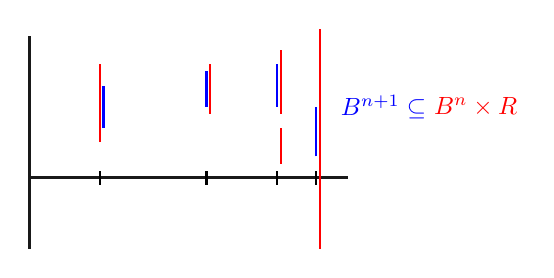
\begin{tikzpicture}[scale=0.9,transform shape]
        \tikzset{
          pics/tick/.style args={#1}{code={
            \draw[line width=0.3mm,inner sep=0mm] (0,-#1) -- (0,#1) ;
            },
          }
        }
          \tikzset{
            cross/.pic ={
              \draw[pic actions,rotate=#1,line width=0.3mm]
                (-3.5pt,0) -- (3.5pt,0)
                (0,-3.5pt) -- (0,3.5pt);
            },
          }
        \draw[black!90,line width=0.4mm] (0,-1) -- ++(90:3cm);
        %AXIS X
        \draw[black!90,line width=0.4mm] (0,0) --++(0:4.5cm); 
        \draw (1,0) pic[rotate=0] {tick={1mm}} node[yshift=-2.5mm,xshift=2mm,scale=1.2] {} ;
        \draw (2.5,0) pic[rotate=0] {tick={1mm}} node[yshift=-2.5mm,xshift=2mm,scale=1.2] {} ;
        \draw (4.05,0) pic[rotate=0] {tick={1mm}} node[yshift=-2.5mm,xshift=2mm,scale=1.2] {} ;
        \draw (3.5,0) pic[rotate=0] {tick={1mm}} node[yshift=-2.5mm,xshift=2mm,scale=1.2] {} ;
        %t1
        \draw[red,line width=0.3mm] (1,0.5) -- (1,1.6);
        \draw[blue,line width=0.3mm] (1.05,0.7) -- (1.05,1.3);
       % \draw[black] (1,0.75) pic {cross={45}} ;
       % \draw[blue] (1,1.5) pic {cross={45}} ;
        %\node[circle,inner sep=0.6mm,fill=black] at (1,1) {};
        %t2
        \draw[blue,line width=0.3mm] (2.5,1) -- (2.5,1.5);
        \draw[red,line width=0.3mm] (2.55,0.9) -- (2.55,1.6);
       % \draw[black] (2.5,1) pic {cross={45}} ;
       % \draw[blue] (2.5,1.25) pic {cross={45}} ;
       % \draw[black] (2.5,1.5) pic {cross={45}} ;

        \draw[blue,line width=0.3mm] (3.5,1) -- (3.5,1.6);
        \draw[red,line width=0.3mm] (3.55,0.2) -- (3.55,0.7);
        \draw[red,line width=0.3mm] (3.55,0.9) -- (3.55,1.8);
       % \draw[black] (3.5,1.5) pic {cross={45}} ;
       % \draw[blue] (3.5,1.35) pic {cross={45}} ;
        %\node[circle,inner sep=0.6mm,fill=blue] at (3.5,1) {};
        %\node[circle,inner sep=0.6mm,fill=black] at (3.5,1.25) {};

        %t4
		\draw[blue,line width=0.3mm] (4.05,0.3) -- (4.05,1);
        \draw[red,line width=0.3mm] (4.1,-1) -- (4.1,2.1);
%        \draw[blue,line width=0.3mm] (4.05,-0.5) -- (4.05,1.8);
       % \draw[black] (4,1.8) pic {cross={45}} ;
       % \draw[blue] (4,0.5) pic {cross={45}} ;
        %\node[circle,inner sep=0.6mm,fill=black] at (4,1.5) {};
        %\node[circle,inner sep=0.6mm,fill=blue] at (4,1.25) {};

        \node[blue] at (5,1) {$B^{n+1}\subseteq$};
        \node[red] at (6.3,1) {$B^{n} \times \mathbb{R}$};
    \end{tikzpicture} 
%    \raisebox{-9mm}{\hspace{-7cm}{More sequences through blue than black restrictions}}  
\end{center}
\end{figure}
In principle the idea is simple. Approximate all $B_n$ with a smaller compact $K_n$ and that's it. Note that finite products of Polish spaces can be made Polish again so that the product $\sigma$-algebra coincides with the Borel-$\sigma$-algebra (for $E=\R$ compare Section \ref{sec:ZV}). We just need to be careful since each $K_n$ gives an approximation error of $\epsilon$ so the error of their combination will add up in $n$. That's why we approximate finer and finer so that the sum of the approximation errors is $\varepsilon$. It is not surprising how to proceed: Chose compact $K_n^*\subseteq \R^n$ such that $K_n^*\subseteq B_n$ and $\mu_n(B_n\backslash K_n^*)\leq 
\frac{\varepsilon}{2^{n+1}}$ and then define
	\begin{align*}
		K_n=(K_1^*\times \R^{n-1})\cap ...\cap (K^*_{n-1}\times \R)\cap K_n^*.
	\end{align*}
	We only need to check that $K_n$ does the job. It follows directly that $K_n\subseteq B_n$ and $K_{n+1}\subseteq K_n\times \R$. The esimates for the probabilities is a bit gnarly but only with standard tricks:
	\begin{align*}
		\mu_n(K_n)\overset{\sigma\text{-add.}}&{=}\mu_n(B_n)-\mu_n(B_n\backslash K_n)\\
		&=\mu_n(B_n)-\mu_n(B_n\backslash ((K_1^*\times \R^{n-1})\cap ...\cap (K^*_{n-1}\times \R)\cap K_n^*))\\
		\overset{\sigma\text{-add.}}&{\geq} \mu_n(B_n)-\mu_n(B_n\backslash(K_1^*\times \R^{n-1}))-...-\mu_n(B_n\backslash K_n^*)\\
		\overset{B_k\subseteq B_1\times \R^{k-1}}&\geq \mu_n(B_n)-\mu_n(B_1\times \R^{n-1}\backslash K_1^*\times \R^{n-1})-...-\mu_n(B_n\backslash K_n^*)\\
		\overset{\text{consistent}}&\geq \mu_n(B_n)-\mu_1(B_1\backslash K_1^*)-...-\mu_n(B_n\backslash K_n^*)\\
		&\geq \varepsilon-\frac{\varepsilon}{4}-...-\frac{\varepsilon}{2^{n+1}}
		\geq \frac{\varepsilon}{2}.
	\end{align*}
Done! \smallskip

We now come to the main part of the proof, the construction of the measure using Carath\'eodory's extension Theorem \ref{KarlTheodor}:	
	\begin{lreminder}
	If $\mu$ is a $\sigma$-additive set-function on a semiring $\mathcal S$, then there is a unique measures $\bar \mu$ on $\sigma(\mathcal S)$ with $\mu(A)=\bar \mu(A)$ for all $A\in \mathcal S$.
	\end{lreminder}
	We proceed in two main steps. First, a semiring $\mathcal S$ with $\sigma(\mathcal S)=\mathcal E^{\otimes I}$ and a set-function $\mu$ are specified. The hard part will be to check the $\sigma$-additivity of $\mu$ for which (as always) a compactness argument is needed. \smallskip	
	
	Define $\mathcal S$ as the set of all finite unions of finitely generated cylinder sets, all sets $C$ that can be written as $\pi^{-1}_J(B_1\times \cdots \times B_n)$ for some finite subset $J=\{t_1,...,t_n\}$ of $I$ and $B_k\in \mathcal E$. The set of finitely generated cylinder is a semiring. The set function $\mu$ on $\mathcal S$ is defined by
	\begin{align}\label{eq_22}
		\mu\big(  \pi^{-1}_J(B_1\times \cdots \times B_n)  \big):=\mathbb{P}_{J}(B_1\times \cdots \times B_n)
	\end{align}
	for all cylinder sets from $\mathcal S$. We now come to the main step of the argument:
	\begin{lstep}
		$\mu$ is a well-defined $\sigma$-additive set-function on $\mathcal S$.
	\end{lstep}
	\textbf{(i) $\mu$ is well-defined}: Suppose a cylinder set $C$ from $\mathcal S$ has two representations 
	 \begin{align}\label{eq_27}
			\pi^{-1}_{J}(B_1\times \cdots \times B_{|J|})=C=\pi^{-1}_{J'}(B'_1\times \cdots \times B'_{|J'|})
	\end{align}
	which can happen if some of the $B_k$ or $B_k'$ are equal to $E$. It is precisely the assumed consistency property (we can cross out all $E$ and delete the time-points) that ensures that the measures of both representations is equal.\smallskip

	\textbf{(ii)} \textbf{$\mu(\emptyset)=0$}: Since $\mu$ is well-defined we are allowed to write $\emptyset$ in some arbitrary way as a finite cylinder set, for instance as $\emptyset = \pi^{-1}_t(\emptyset)$ for arbitrary $t\in I$. But this leads to $\mu(\emptyset)=\P_{\{t\}}(\emptyset)=0$.\smallskip

	\textbf{(iii)} \textbf{$\mu$ is finitely additive}: It is enough to prove additivity for two disjoint cylinder sets, finite (but not infinite!) additivity then follows from induction. Suppose $A_1\in \mathcal E^{\otimes |J_1|}$ and $A_2\in \mathcal E^{\otimes |J_2|}$ are boxes such that the corresponding cylinder sets are disjoint, i.e. $\pi_{J_1}^{-1}(A_1)\cap \pi_{J_2}^{-1}(A_2)=\emptyset$. The trick is to use that finitely generated sets have different representations by adding further indices without imposing restrictions (see the drawing). 
	\begin{figure}[h]
		\begin{center}
			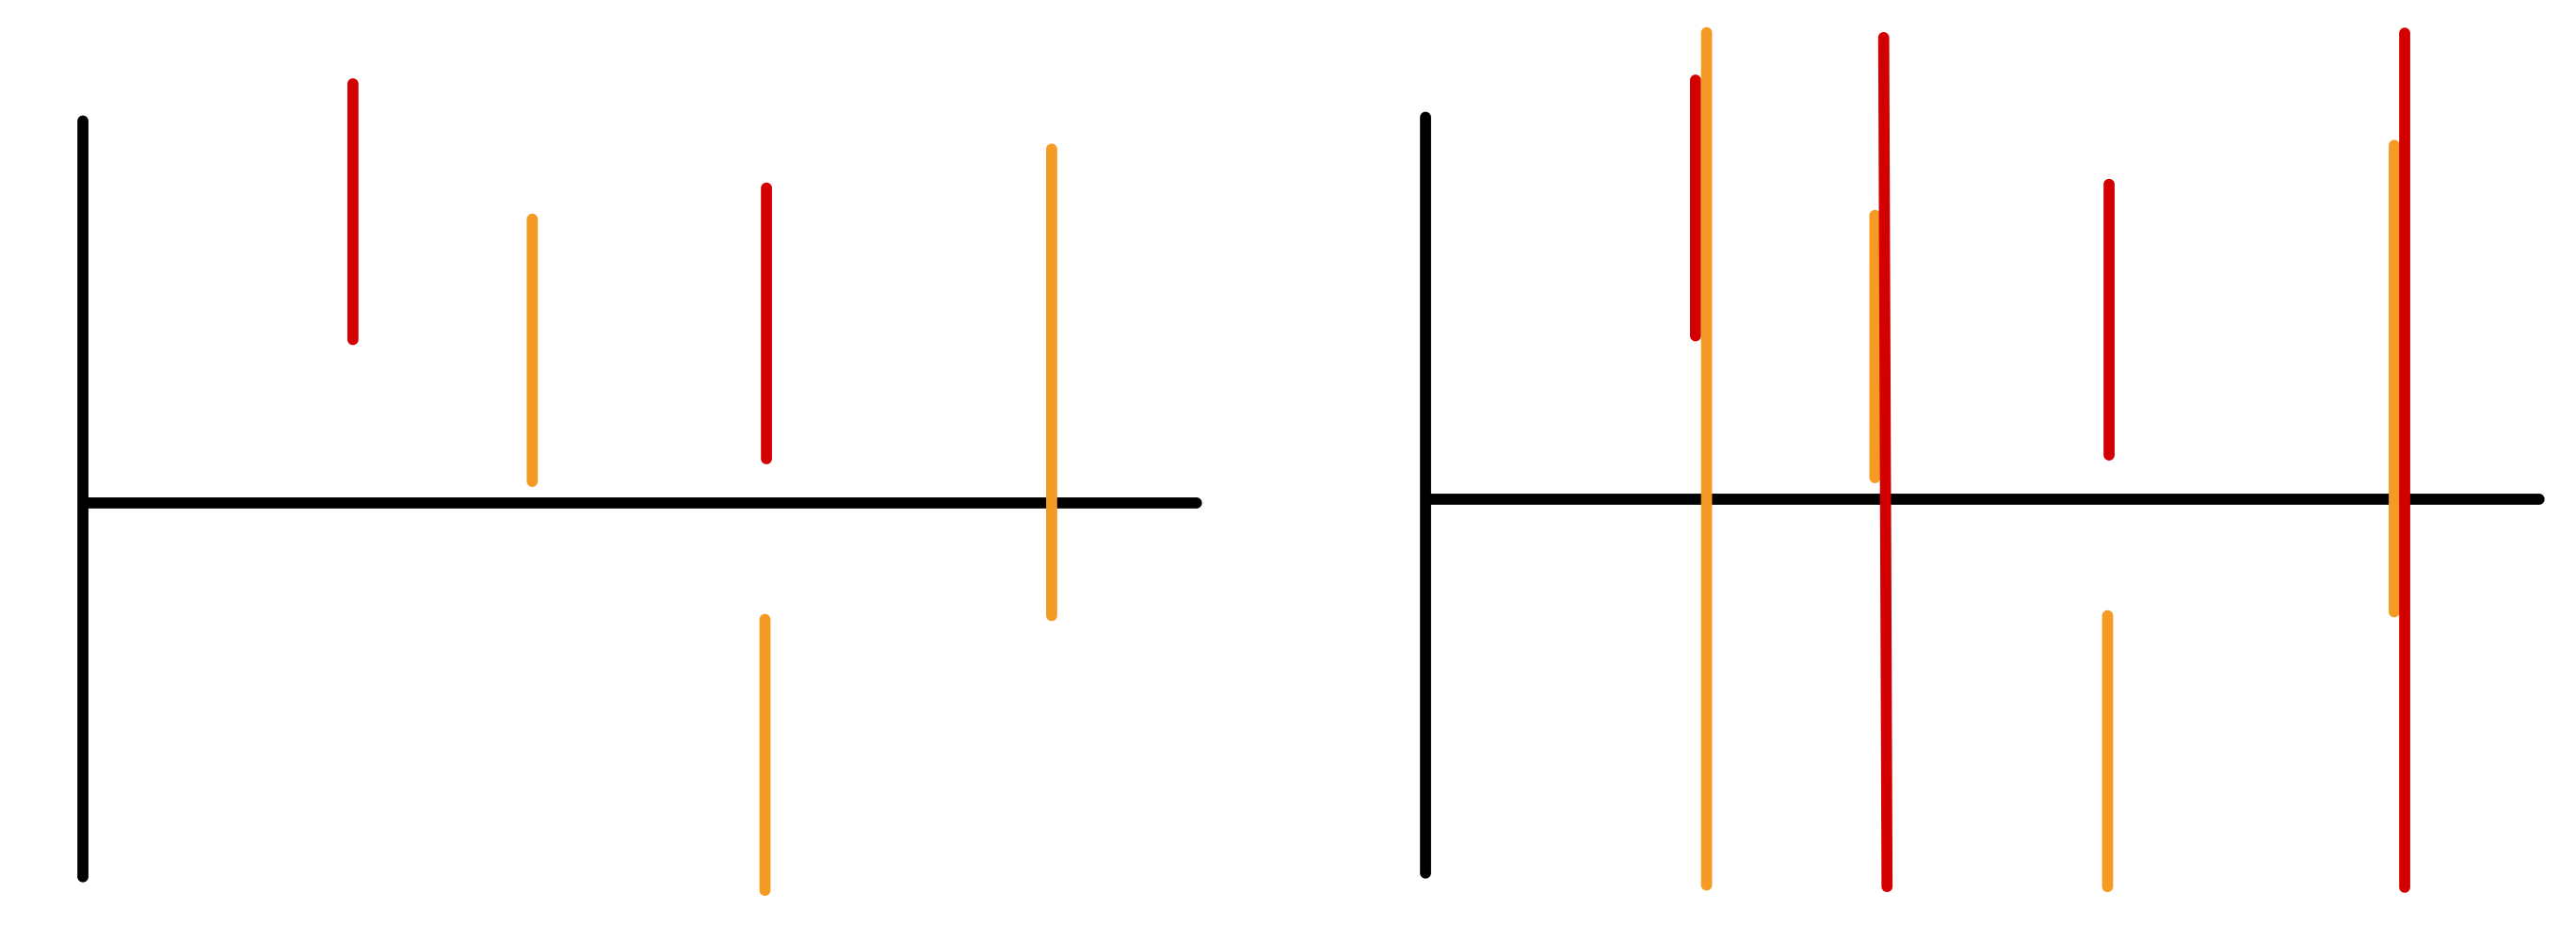
\includegraphics[scale=0.08]{vereinigung.jpeg}
			\caption*{$A_1, A_2$ rewritten as $\tilde A_1, \tilde A_2$ spanned by the same time-points $J=J_1\cup J_2$}
		\end{center}
		\end{figure}

	Let us denote $J=J_1\cup J_2$ and $\tilde A_1=\pi_{J,J_1}^{-1}(A_1)$, $\tilde A_2=\pi_{J,J_2}^{-1}(A_2)$ as in the drawing. Then the finitely generated sets of paths $\pi^{-1}_J(\tilde A_1)$ and $\pi^{-1}_J(\tilde A_2)$ are disjoint and the definition of $\mu$ gives
	\begin{align*}
		\mu(\pi_{J_1}^{-1}(A_1)\cupdot\pi_{J_2}^{-1}(A_1))\overset{\text{Def. $\mu$}}&{=}\P_J(\tilde A_1\cupdot \tilde A_2)\\
		\overset{\P_J\text{ measure}}&{=}\P_J(\tilde A_1)+\P_J(\tilde A_2)\\
		\overset{\text{consistency}}&{=}\P_{J_1}(A_1)+\P_{J_2}(A_2)\\
		\overset{\text{Def. $\mu$}}&{=}\mu(\pi^{-1}_{J_1}(A_1))+\mu(\pi^{-1}_{J_2}(A_2)).
	\end{align*}
	\textbf{(iv)} \textbf{$\mu$ is a $\sigma$-additive set-function}: Assume $C_1,C_2,...$ is a sequence of disjoint cylinder sets from $\mathcal S$ such that $C:=\cupdot_{k=1}^\infty C_k\in \mathcal S$. We have to prove that $\mu(C)=\sum_{k=1}^\infty \mu(C_k)$. The finite additivity implies 
\begin{align*}
	\mu(C)=\mu\big(C\,\backslash \cupdot_{k=1}^N C_k\big)+\mu\big(\cupdot_{k=1}^N C_k\big)=\mu\big(C\,\backslash \cupdot_{k=1}^N C_k\big)+\sum_{k=1}^N\mu\big( C_k\big).
\end{align*}
Hence, it suffices to prove that
\begin{align}\label{lim:D}
	\lim_{n\to\infty}\mu(D_n)=0,
\end{align}
where $D_n=C\,\backslash \cupdot_{k=1}^n C_k\in \mathcal S$. One might be tempted to say this is just continuity of measures, and, in fact, continuity of measures plus finite additivity gives $\sigma$-additivity. To prove \eqref{lim:D} we use a compactness argument involving the steps above. Since finitely generated sets form a semiring, $(D_n)_{n\in\N}$ is a decreasing sequence of finite cylinder sets. The sequence $\mu(D_n)$ is decreasing (monotonicity of set-functions follows from finite additivity!) to some number $\varepsilon$. Let us assume $\varepsilon>0$ and construct a contradiction. The contradiction will be that 
\begin{align}\label{contradiction}
	\cap_{k=1}^\infty D_k\neq \emptyset
\end{align}
which is absurd because it would contradict $C=\cupdot_{k=1}^\infty C_k$. Since the $D_n$ are decreasing finitely generated cylinder sets we may assume without loss of generality that
\begin{align*}
	D_n=\pi^{-1}_{\{t_1,...,t_n\}}(B_n)
\end{align*}
for a sequence $t_1,t_2,...$ and boxes $B_n\subseteq \mathcal E^{\otimes n}$ satisfying $B_{n+1}\subseteq B_{n}\times E$. To understand what we are doing let us think what could go wrong. Since the cylinder sets are nested it could a priori be that there is a "hole"{} in all of them and the intersection only contains a function contained in the hole and thus does not belong to the intersection (see the drawing).
\begin{figure}[h]
	\begin{center}
		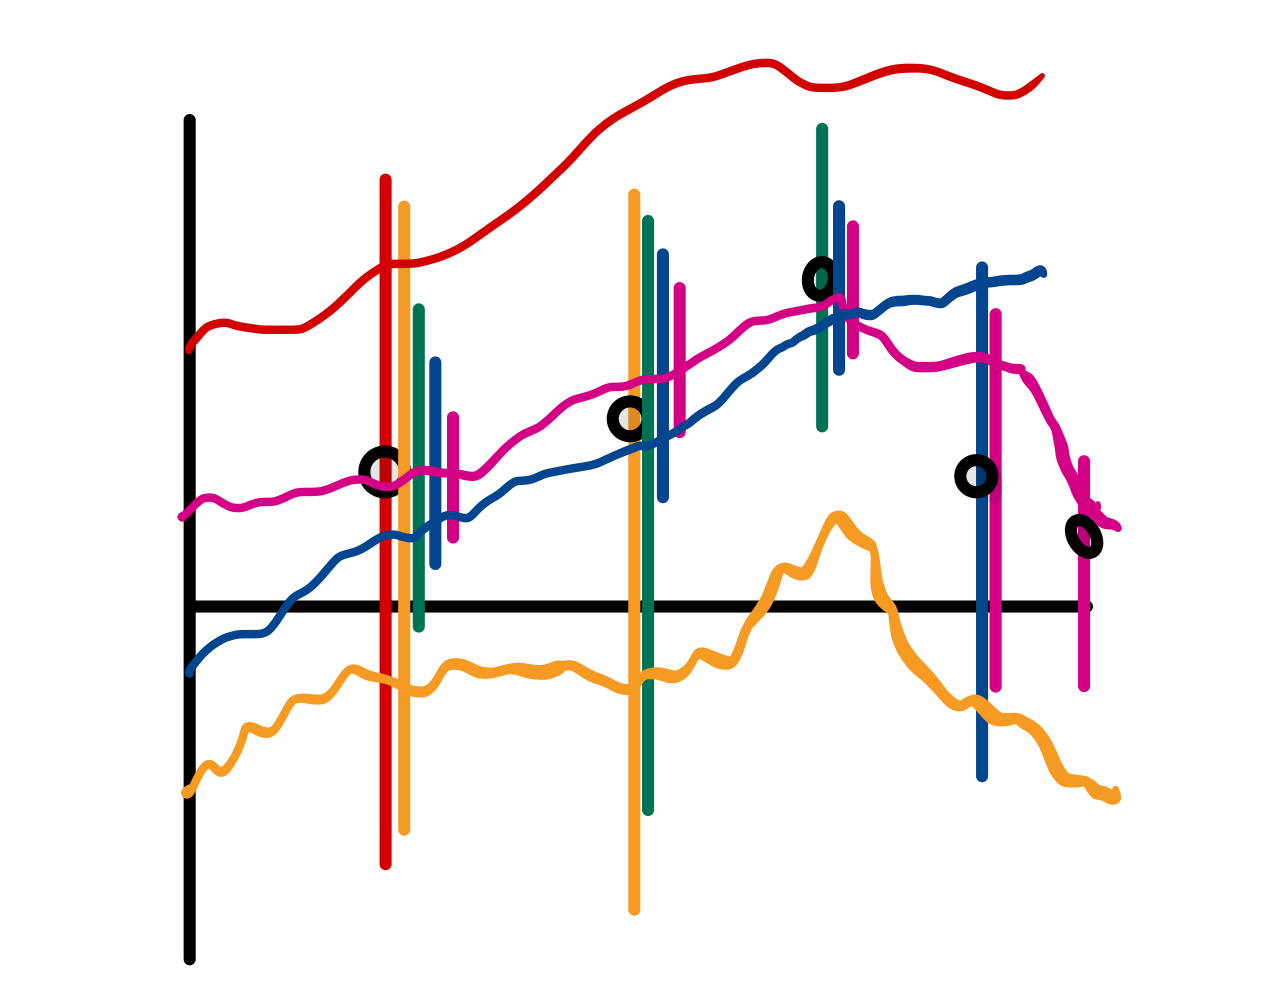
\includegraphics[scale=0.1]{bunt.jpeg}
		\caption*{A decreasing sequence of cylinder sets that might have an empty intersection}
	\end{center}
	\end{figure}

It is the regularity (in particular the closeness of the approximation) from inside which prevents us from such a situation. Due to the step above we can replace without loss of generality the sets $B_n$ by compact sets $K_n\subseteq B_n$ (changing $\varepsilon$ into $\varepsilon/2$). Since the $K_n$ are non-empty (they have positive measures), we can pick vectors $x^n=(x_1^n,...,x_n^n)\in K_n$. The $K_n$ are nested, thus, the entire sequence $(x_1^n)$ lies in the compact set $K_1$. Hence, there is a convergent subsequence $(x_1^{n'_k})$ that converges to some $x_1\in K_1$. Next, the sequence $(x_1^{n'_k}, x_2^{n'_k})$ is contained in $K_2$, thus, there is another converging subsequence $(x_1^{n_k''}, x_2^{n_k''})$ that converges to some $(x_1,x_2)\in K_2$. Continuing like that (diagonal argument) we obtain a sequence $(x_n)_{n\in\N}$ in $E$ such that $(x_1,x_2,...,x_n)\in K_n\subseteq B_n$ for all $n\in\N$. But then there is a function $f:I\to E$ passing through $x_k$ at times $t_k$ (define $f$ arbitrarily away from $\{t_1,...\}$), hence, $f\in \cap_{k=1}^\infty D_k$ (there is no hole in the intersection). Hence, \eqref{contradiction} is matched and we have our contradiction.
\end{proof}
Here is a small point regarding the proof to keep in mind for the following discussion of continuous functions. In principle $\{t_1,t_2,...\}=\Q$ is possible and the functions to construct the contradiction pass through given sets spanned on $\Q$. Depending on the sets $K_n$ there is no guarantee that a continuous function $f$ can be chosen for the contradiction, thus, a similar argument can not be used if one tried to carry out the same proof for continuous functions instead of generic functions. 

\subsubsection{(C) Path valued random variables and stochastic processes}
The third step in the triology of measure theory is to understand the connection of stochastic processes and path-valued random variables. We start with the natural generalization of Proposition \ref{zweiInterpr}:
\begin{laussagewerkzeug}
\begin{prop}\label{zweiInterprb}
		$X=(X_t)_{t\in I}$ is an $E$-valued stochastic process on $(\Omega, \mathcal A, \P)$ if and only if the mapping $$X:\omega\mapsto \big(t\mapsto X_t(\omega)\big)$$ is a path-valued random variable.
	\end{prop}
\end{laussagewerkzeug}
A bit of care is needed to explain the statement. If $(X_t)$ is a family of random variables it is clear how the path-valued mapping has to be interpreted. Fix $\omega$ and then consider all values $X_t(\omega)$ as a function in $t$. The converse is a bit more tricky. To switch back from the path-valued valued mapping to a family of $E$-valued mappings one needs to evaluate $X$ at all times $T$, formalized using the projections: $X_t:=\pi_t(X)$. 
\begin{proof}[Proof]
	\begin{itemize}
		\item["$\Leftarrow$":] 
		For $B \in \mathcal E$ we have 
\[ X_t^{-1} (B) = X^{-1}(\pi_t^{-1}(B)) \in \mathcal A, \]
because $\pi_t^{-1}(B)$ is a finitely generated cylinder set and $X$ is $(\mathcal A, \mathcal E^{\otimes I})$-measurable.
		\item["$\Rightarrow$":] Using Proposition \ref{S2} the measurability property only needs to be checked on an arbitrary generator. We use the cylinder sets $\pi_t^{-1}(B)$ generated by single time-points:
		\begin{align*}
			X^{-1}(\pi_t^{-1}(B)) =\{\omega \in \Omega: X_t(\omega)\in B\}=X^{-1}_t(B)\in \mathcal A.
		\end{align*}
		Hence, seen as a path-valued random variable $X$ is measurable.
	\end{itemize}
\end{proof}
Next, the notion of the law from random variables and random vectors is generalized to stochastic processes:
\begin{ldef}
\begin{deff}\label{def:SP}
		Suppose $X$ is an $E$-valued stochastic process on $(\Omega, \mathcal A, \P)$. 
		\begin{enumerate}[label=(\roman*)]
			\item The image measure 		
		\begin{align*}
			\P^X(A):=\P(X\in A),\quad A\in \mathcal E^{\otimes I},
		\end{align*}
		is called the \textbf{law of $X$}.
		\item For a finite subset $J=\{t_1,...,t_k\}$ of $I$ we call the distribution of $(X_{t_1},...,X_{t_k})$ a \textbf{finite-dimensional distribution (fdd) of $X$} and write
		\begin{align*}		
			\P^X_{t_1,...,t_k}\sim (X_{t_1},...,X_{t_k}).
		\end{align*}
	\end{enumerate}
\end{deff}
\end{ldef}
The fdds can be computed from the law by restricting to finite cylinder sets:
\begin{align*}
	\P^X_{t_1,...,t_k}(B_1\times ...\times B_k)=\P(X_{t_1}\in B_1,..., X_{t_k}\in B_k)
&=\P^X(\pi_{t_1,...,t_k}^{-1}(B_1\times ... \times B_k)),
\end{align*}
for $t_i\in I, B_i\in \mathcal E$.
\begin{lWarnhinweis}
	The law of a stochastic process is a delicate object, a measure on the path space. Usually the law does not play a big role	and we are almost exclusively thinking about the fdds.
\end{lWarnhinweis}
The reason why it is always sufficient to think about the fdds is the following proposition, both concepts are equivalent.
\begin{laussagewerkzeug}
\begin{prop}
		The law of a stochastic process $X$ is uniquely determined by all it's finite-dimensional distributions $\P^X_{t_1,...,t_k}=\P(X_{t_1}\in \cdot, ..., X_{t_k}\in \cdot)$.
\end{prop}
\end{laussagewerkzeug}
\begin{proof}[Proof]
	This follows from the abstract theory of the previous section. Since all finitely generated cylinder sets generate the path $\sigma$-algebra $\mathcal E^{\otimes I}$ and are intersection stable the measure $\P^X$ is uniquely determined on all sets $\pi_{t_1,...,t_k}^{-1}(B_1\times \cdots \times B_k)$.
\end{proof}
It is crucial to assume that \textbf{all} finite-dimensional distributions are equal. If $X$ is a symmetric random variable, then $(X,-X)$ and $(X,X)$ have different laws but the same one-dimensional distributions.
\begin{ldef}
\begin{deff}
	Two stochastic processes $X$ and $Y$ with index set $I$ have the \textbf{same law} if $\P^X=\P^Y$. Equivalently, we say they have the \textbf{same finite-dimensional distributions} if $\P^X_{t_1,...,t_k}=\P^Y_{t_1,...,t_k}$ for all finite subsets $\{t_1,...,t_k\}$ of $I$ and write $\P^X\overset{\text{fdd}}{=}\P^Y$.
\end{deff}
\end{ldef}
Just as for random variables, the case $|I|=1$, two stochastic processes with same law do not need to be defined on the same probability space. The notion of equality in law is the weakest equality notation available, stronger notions will be discussed in the next section. \smallskip

If you remember well the previous 300 pages of these lecture notes you will know what is up next. The existence of stochastic processes using the canonical constructions. Earlier versions covered the cases $|I|=1$, $|I|<\infty$, and $I=\N$. Here is the general version for arbitrary $I$ only assuming $E$ is Polish.
\begin{lsuperwichtigersatzExistence}
	\begin{theorem}[Canonical construction on $E^{I}$]\label{KolmogorovProcess}
		Suppose $E$ is a Polish metric space, $I$ an index set, and $\{\P_J:|J|<\infty\}$ a consistent family of finite-dimensional distributions. Then there is a stochastic process $X$ on some probability space $(\Omega, \mathcal A, \P)$ with marginals $\P_J^X=\P_J$ for all finite sets of times.
	\end{theorem}
\end{lsuperwichtigersatzExistence}
\begin{proof}[Proof]
	In the usual way we construct a probability space and a (path-valued) random variable:
	\begin{itemize}
		\item $\Omega=E^I$
		\item $\mathcal A=\mathcal E^{\otimes I}$
		\item $\P=\P^X$, the measure on $\mathcal E^{\otimes I}$ obtained from the consistent family using Theorem \ref{Kolm}.
		\item $X$ is the identity mapping from $E^I$ to $E^I$.
		\item $X_t=\pi_t(X)$ the evaluation of $X$ at time $t$.
	\end{itemize}
	The measurability of $X$ is clear (preimages of measurable sets are the same measurable sets) and the law is $\P^X=\P$ which has the good finite-dimensional distributions by construction.
\end{proof}
People tend to like the canonical construction as it always works (justifying the name canonical) but there are very good reasons to avoid the canonical construction if possible. For instance the statement "{}$X$ is $\P$-almost surely continuous/differentiable/constant/etc."{} is problematic for a real-valued process on the canonical probability space because such events are not measurable in $\mathcal B(\R^{[0,\infty)})$, hence, no probabilities can be defined. In fact, the problem can be avoided using a better definition of nullsets than the one we gave in Definition \ref{def:Nullmenge}, compare also the footnote after the definition.
\begin{lWarnhinweis}
	From now on a set $A\subseteq\Omega$ is called a nullset if there is a measurable set $B$ with $A\subseteq B$ and $\P(B)=0$. A property $E$ holds $\P$-almost surely, if $\{\omega: E(\omega) \text{ does not hold}\}$ is contained in a measurable set with measure $0$, or, equivalently, if $\{\omega: E(\omega) \text{ holds}\}$ contains a measurable set with measures $1$.
\end{lWarnhinweis}
There is no problem for the discussion in all previous chapters as all previous nullsets of interest $\{X=Y\}$, $\{X\geq 0\}$, $\{X_n \text{ converges}\}$, etc. were measurable themselves. We will return a few times to the measurability problems on the path space but now want to get towards examples. Here is a first important class of stochastic processes that can be constructed using the theory developed above.
%\begin{example}[iid sequences of random variables]
%	Suppose $E$ is a Polish metric space, $\P$ is a distribution on $(E,\mathcal B(E))$, and suppose $I=\N$. Then define for all natural numbers $t_1<...<t_n$ the finite product measures
%	\begin{align*}
%		\P^{t_1,...,t_n}(B_1\times \cdots \times B_n):=\P(B_1)\cdot... \cdot \P(B_n),\quad B_i\in \mathcal E.
%	\end{align*}
%	Since $\P(E)=1$ it follows immediately that the family is consistent:
%	\begin{align*}
%		\P^{t_1,...,t_{n+1}}(B_1\times \cdots \times B_n\times E)=\P(B_1)\cdot... \cdot \P(B_n)\cdot \P(E)=\P^{t_1,...,t_{n}}(B_1\times \cdots \times B_n).
%	\end{align*}
%	Hence, there is a stochastic processes $X$ indexed by $\N$ with finite-dimensional distributions $\P^{t_1,...,t_n}$. What does this mean? If we interpret the stochastic process $(X_t)_{t\in\N}$ as a family (here: sequence) of random variables $X_1,X_2,...$ then  
%	\begin{align*}
%		\P(X_1\in B_1,..., X_n\in B_n)&=\P^{1,...,n}_X(B_1\times \cdots \times B_n)\\
%		&=\P(B_1)\cdot ... \cdot \P(B_n)\\
%		&=\P_X^{1} (B_1)\cdot ... \cdot \P_X^{n}(B_n)=\P(X_1\in B_1)\cdot ...\cdot \P(X_n\in B_n).
%	\end{align*}
%	This means we constructed a sequence of iid $E$-valued random variables with prescribed distribution $\P$.
%\end{example}
\begin{ldef}
	\begin{deff}
		A stochastic process $(X_t)_{t\in I}$ is called a \textbf{Gaussian process} if all finite-dimensional distributions $(X_{t_1},...,X_{t_k})$ are multi-variate Gaussian. We call $$m(t):=\E[X_t],\quad t\in I,$$ the mean-function of $X$ and $$K(t,s):=\E[(X_t-m(t))(X_s-m(s))],\quad t,s\in I,$$ the covariance function of $X$. A Gaussian process is called \textbf{centered} if $m\equiv 0$.
	\end{deff}
\end{ldef}
The special case $I=\{1,...,d\}$ shows that Gaussian processes are generalizations of Gaussian vectors (or random variables for $d=1$). Since Gaussian vectors are uniquely determined by mean an covariances and a stochastic processes by its fdds, a Gaussian process is uniquely defined through $m$ and $K$. Recalling the discussion at the end of Chapter \ref{chapter:CV} the function $K$ automatically has a lot of structure, all matrices $(K(t_i,t_j))_{i,j=1,...k}$ of covariances are symmetric and positive semidefinite for all finite choices $t_1,...,t_k\in I$. This naturally leads to the notion of positive semidefinite functions on $I\times I$ as a generalization of positive semidefinite matrices for $|I|<\infty$. A symmetric function $K:I\times I\to \R$ is called positive semidefinite if 
\begin{align*}
	\sum_{i,j=1}^ka_ia_jK(t_i,t_j)\geq 0,\quad \text{for all }k\in\N, t_i, t_j\in I,\text{ and }a\in \R^n.
\end{align*}
 Note that in the case $I=\{1,...,d\}$ this is exactly the definition of a symmetric positive semidefinite matrix. Here are some examples for symmetric positive semidefinite functions on $I=[0,\infty)$:
\begin{align*}
	K(t,s)=\delta_{t,s},\quad K(t,s)=t\wedge s:=\min(t,s), \quad K(t,s)=\exp(-|t-s|).
\end{align*}
It is surprisingly complicated to check that such simple functions are positive semidefinite. Either the definition can be checked directly by some induction, $K(t,s)=\varphi(t-s)$ is the characteristic function of some random variable (compare Bochner's theorem \eqref{Bochner}), or some other clever trick is needed. Nonetheless, there are many examples of symmetric positive semidefinite functions in the literature. The covariance function is very closely related to properties of the sample paths. For example $\delta_{s,t}$ leads to completely chaotic paths as all $X_s, X_t$ are independent while $K(s,t)=\varphi(|t-s|)$ leads to smooth paths if $\varphi$ decays slowly because it makes $X_s$ and $X_t$ stronger correlated if $\varphi$ decays slower.
\begin{figure}[h]
	\begin{center}
		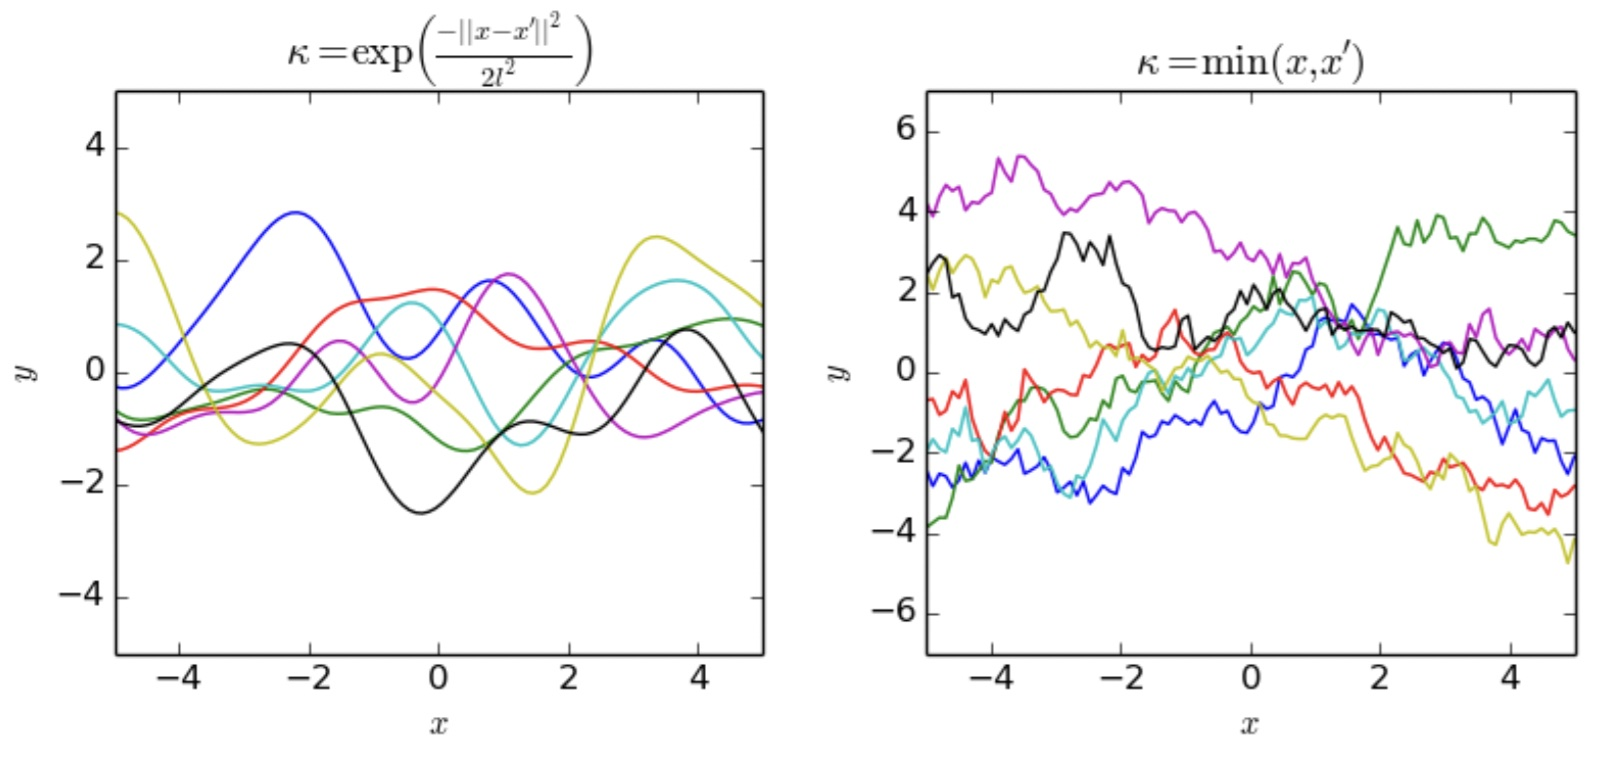
\includegraphics[scale=0.17]{Gaussian.jpeg}
	\end{center}
	\end{figure}
Gaussian processes are the prime example for the power of Kolmogorov's construction theorem of stochastic processes. Positive semidefinite covariance function is clearly a necessary condition for the existence of a stochastic process, but it is also sufficient for the existence of a Gaussian process with covariance function $K$.
\marginpar{\textcolor{red}{Lecture 22}}
\begin{lSatzHerz}
	\begin{satz}
	Let $m:I\to \R$ and $K:I\times I\to \R$ be symmetric and positive semidefinite. Then there is a Gaussian process $(X_t)_{t\in I}$ with mean-vector $m$ and covariance function $K$.
	\end{satz}
\end{lSatzHerz}
\begin{proof}[Proof]
	For arbitrary $J\subseteq I$ finite define the finite-dimensional Gaussian random distributions $\P_J\sim \mathcal N(m_J,\Sigma_J)$ with mean vector $m_J=m((t_1),...,m(t_n))$ and covariance matrix $\Sigma_J=(K(t_i,t_j))_{i,j\in J}$. The definition of a positive semidefinite function ensures that $\Sigma_J$ is a positive semidefinite matrix for all choices of $J$. To check the consistency of $\{\P_J:|J|<\infty\}$ we use the characteristic function and show that $\varphi_{\P_J\circ \pi_{J,J'}^{-1}}= \varphi_{\P_{J'}}$ for all $J'\subseteq J$. This is not hard as the characteristic functions of Gaussian vectors have a nice form. The computation looks more complicated than it is, it is mostly about notation and multiplying matrices with vectors that have some zeros. For a vector $t\in \R^{|J'|}$ we define $\hat t\in \R^{|J|}$ as the enlarged vector which has zeros at $J\backslash J'$ and coincides with $t'$ on $J'$. The characteristic functions can now be computed using the transformation formula from Theorem \ref{trafo} and the characteristic functions of Gaussian random vectors:
	\begin{align*}
		\varphi_{\P_J\circ \pi_{J,J'}^{-1}}(t)
		&=\int_{\R^{|J'|}} e^{i\langle t,x \rangle} \P_J\circ \pi_{J,J'}^{-1}(\mathrm d x)\\
		\overset{\text{trafo.}}&{=}\int_{\R^{|J|}} e^{i\langle t,\pi_{J,J'}(y) \rangle} \P_J(\mathrm d y)\\
		\overset{\text{compare zeros}}&{=}\int_{\R^{|J|}} e^{i\langle \hat t,y \rangle} \P_J(\mathrm d y)\\
		&=e^{i\langle \hat t,m_J\rangle }e^{-\frac{1}{2}\langle \hat t, \Sigma_{J} \hat t \rangle}\\
		\overset{\text{compare zeros}}&{=}e^{i\langle t,m_{J'}\rangle } e^{-\frac{1}{2}\langle t, \Sigma_{J'} t\rangle} =\varphi_{\P_{J'}}(t),\quad \forall t\in \R^{|J'|}.
	\end{align*}
	Since characteristic functions uniquely determine distributions it follows that $\P_J\circ \pi_{J,J'}^{-1}=\P_{J'}$, the consistency is proved. The existence of the Gaussian process with finite-dimensional distributions $\P_J$ now follows from Theorem \ref{KolmogorovProcess}.
\end{proof}
There is a second enormously important class of stochastic processes that can be constructed using the Kolmogorov extension theorem. Continuous- (or discrete-) time Markov process with given transition probabilities can be constructed by writing down the finite-dimensional distributions that can be guesses from the Markov property. 
\begin{luebung}
	Use the formula
	\begin{align*}
		\P(X_{1}=e_1,...,X_{n}=e_n)=\mu(e_1)A_{e_1,e_2}\cdots A_{e_{n-1},e_n},
	\end{align*}
	to construct a discrete-time Markov chain $(X_n)_{n\in\N}$ on the finite state-space $E=\{e_1,...,e_d\}$ with initial distribution $\mu$ and transition matrix $A$.
\end{luebung}
The general case for continuous time and/or continuous space will be covered in lectures on Markov processes.


\subsection{Stochastic processes with continuous sample paths}\label{sec:continuouspaths}

So far we developed a tool to construct stochastic processes with given finite-dimensional distributions using the canonical construction based on the Kolmogorov extension theorem. The story is not over, yet, if we are interested in stochastic processes with regular (e.g. continuous) sample paths. One of the motivations to keep the weak convergence chapter more general than just $\R^d$ was to introduce a notion of convergence of stochastic processes. In order to do so we must be able to interpret a stochastic process as a random variable with values in a Polish space. So far, it is unclear what that Polish space could be because the generic path space $\R^{I}$ has no topological structure what so ever. The aim of this section is two-fold. First, we first explain the path-space of continuous real-valued functions and stochastic processes with continuous paths, secondly, we discuss ways of constructing such processes. Unfortunately, it's not possible to prove a generic construction theorem like the Kolmogorov extension theorem, the proof of the Kolmogorov extension theorem breaks down if used on continuous functions. Instead, we will introduce a method to modify stochastic processes without path regularity into processes with (H\"older-)continuous sample paths. 

\subsubsection{The path space of continuous functions}
The space of continuous functions on a compact set (here: compact interval) has already been studied in the previous chapter. It is well-known from basic analysis that $C([0,T])$ is complete, the Stone-Weierstra\ss{} theorem applied to polynomials with rational coefficients also shows that $C([0,T])$ is separable. Hence, $(C([0,T]), ||\cdot ||_\infty)$ is a Polish space and as such suitable for the theory developed in the previous chapter. As we are mostly interested in stochastic processes indexed by $[0,\infty)$ it is important to know that also continuous functions indexed by $[0,\infty)$ can be made into a Polish space:
\begin{laussagewerkzeug}
\begin{prop}\label{prop:C}
	\begin{enumerate}[label=(\roman*)]
		\item If we define
			\begin{align*}
				d(f,g)\coloneqq \sum_{k=1}^{\infty} \frac{d_k(f,g)\wedge 1}{2^k},\quad d_k(f,g) = \sup_{x\in [0,k]} \lvert f(x) - g(x)\rvert,
			\end{align*}
		then $d$ is a metric on $C([0,\infty))$. 
		\item $d$ metrizes convergence on compacts, that is
		\begin{align*}
			\lim_{n\to\infty} d(f_n,g)=0\quad \Leftrightarrow \quad \lim_{n\to\infty}\sup_{x\in K}|f_n(x)-g(x)|=0\text{ for all }K\text{ compact.}
		\end{align*}
		\item $( C([0,\infty)),d )$ is a Polish metric space.
	\end{enumerate}
\end{prop}
\end{laussagewerkzeug}
Note that $||f||_\infty=\sup_{t\geq 0}|f(t)|$ cannot be used on $C([0,\infty))$ as the supremum must not be finite ($[0,\infty)$ is not compact), for instance all polynomials are unbounded on $[0,\infty)$. We could try to use the bounded continuous functions instead but $(C_b([0,\infty)),||\cdot||_\infty)$ is not separable and additionally bounded functions are not enough for our purposes. For these reasons we work with the metric $d$ from the proposition.
\begin{proof}[Proof]
(i) It should be known from basic analysis that $d_k$ is a metric on $C([0,k])$, the properties of a metric space then follow immediately for $d$.\smallskip

(ii) It follows from the Heine-Borel Theorem that all compact subsets of $[0,\infty)$ are bounded. \smallskip
		
		"$\Rightarrow$": Suppose $\lim_{n\to\infty} d(f_n,g)=0$. Chose $K$ compact and some $k$ such that $K\subseteq [0,k]$. Since $\frac{d_k(f_n,g)\wedge 1}{2^k}\leq d(f_n,g)$ the uniform convergences on $[0,k]$ (and thus $K$) follows.\smallskip
	
		"$\Leftarrow$": The truncation by $1$ allows to apply the dominated convergence theorem to get
		\begin{align*}
			\lim_{n\to\infty}d(f_n,g) \overset{\text{DCT}}{=} \sum_{k=1}^{\infty} \lim_{n\to \infty} \frac{d_k(f_n,g)\wedge 1}{2^k}=0,			
		\end{align*}
			since all $[0,k]$ are compact.\smallskip

		 (iii) Separability: The set of polynomials with rational coefficients restricted to $[0,n]$ is countable and dense in $(C([0,n]),||\cdot||_\infty)$, see the discussion below Theorem \ref{Weierstrass_approx}. Now suppose $f\in C([0,\infty))$ and $\varepsilon>0$. Then there is some $n$ such that $\sum_{k=n}^\infty \frac{1}{2^k}<\frac{\varepsilon}{2}$. Choosing a polynomial $p$ with rational coefficients such that $\sup_{t\in [0,n]}|f(x)-p(x)|<\frac{\varepsilon}{2}$ then shows that $d(f,p)<\varepsilon$.\smallskip		 
		 
		Completeness: Suppose $(f_n)_{n\in\mathbb{N}}$ is Cauchy. By the definition of the metric, $(f_n)_{n\in\mathbb{N}}$ restricted to $[0,k]$ is also Cauchy in $(C([0,k]),||\cdot||_\infty)$. Since $( C([0,k]), ||\cdot||_\infty)$ is complete, for all $k\in\N$ there is a uniform (continuous) limit $g_k$ on $[0,k]$. Let us define a function $g:[0,\infty)\to \R$ as $g_k(x)$ for $x\in [0,k]$ and some $k>x$. Since $g_k = g_{k'}$ on $[0,k]$ for all $k' \geq k$ this construction is well-defined. Using dominated convergence once more yields
		\begin{align*}
			\lim_{n\to\infty}d(f_n,g) \overset{\text{DCT}}{=} \sum_{k=1}^{\infty} \lim_{n\to\infty} \frac{d_k(f_n,g)\wedge 1}{2^k} = 0.
		\end{align*}
		Hence, $( C([0,\infty)),||\cdot||_\infty)$ is complete.
\end{proof}
Since $\big( C([0,\infty)),d \big)$ is a Polish metric space there is a natural $\sigma$-algebra on $E$, the Borel-$\sigma$-algebra generated by all open sets. Such a $\sigma$-algebra has much more structure than the product $\sigma$-algebra on the generic path space $\R^{[0,\infty)}$. As an example, all probability measures are inner regular. In contrast, $\mathbb{R}^{[0,\infty)}$ is topologically nothing useful. That's why the $\sigma$-algebra is not the topological $\sigma$-algebra induced by open sets (what are open sets without a topology?) but defined "by hands". Even though $\cB(C([0,\infty)))$ is structurally much more rich there is a lot of similarity to the generic path $\sigma$-algebra. For example both $\sigma$-algebras have the same simple generators, the cylinder sets, but now cylinder sets of continuous functions.
\begin{laussagewerkzeug}
\begin{prop}
	$\cB ( C([0,\infty)))$ is generated by the cylinder sets of continuous functions, i.e. 
	\begin{align*}
		\cB \big( C([0,\infty))\big) &= \sigma( \{\pi_t^{-1}(B):t \geq 0, B\in  \mathcal B(\R) \}),\\
				&= \sigma \big( \{ \text{finitely generated cylinder sets of continuous functions} \}\big),
	\end{align*}
	where $\pi_t:C([0,\infty))\to \R, f\mapsto f_t,$ are the projections at time $t$.
\end{prop}
\end{laussagewerkzeug}
In order to avoid confusion with the product $\sigma$-algebra on all generic functions let us emphasize the difference of projections on all continuous functions and generic functions. 
\begin{figure}[h]
	\begin{center}
	\begin{tikzpicture}
			\tikzset{
			  pics/tick/.style args={#1}{code={
				\draw[line width=0.3mm,inner sep=0mm] (0,-#1) -- (0,#1) ;
				},
			  }
			}
			\tikzset{
			  pics/intervall/.style args={#1}{code={
				\draw[red,line width=0.2mm] (0,0) -- ++(0,#1) 
				node[rotate=90,sloped,inner xsep=0.8mm,inner ysep=0,pos=1,fill,red] (E) {}
				node[rotate=90,sloped,inner xsep=0.8mm,inner ysep=0,pos=0,fill,red] (E) {};
			  },
			}
			}
			%AXIS Y
			\draw[black!90,line width=0.4mm] (0,-.2) -- ++(90:2cm);
			%AXIS X
			\draw[black!90,line width=0.4mm] (0,0) --++(0:3.5cm);  
			\draw (2,0) pic[rotate=0] {tick={1mm}} node[yshift=-2.5mm,xshift=2mm,scale=1.2] {$t$} ;
	
			\draw[red,line width=0.4mm] (2,-0.2) --++(90:1.5cm) node[xshift=2mm,pos=1,red] {$B$};
			
		  %func 1 
		  \draw[blue,line width=0.3mm] (0,1.5) .. controls (1.5,-0.8) and  (2.5,3) .. (3.5,-0.2);
		  %func 3
		  \draw[darkgreen,line width=0.3mm] (0,0.2) .. controls (1,0.3) and (2,-0.3) .. (3.5,0.2);
		  \draw[purple,line width=0.3mm] (0,-0.2) .. controls (1,1.3) and (2,-0.3) .. (3.5,0.2);
		  \draw[orange,line width=0.3mm] (0,0.5) .. controls (1,1.3) and (2,-0.3) .. (3.5,1);
		\end{tikzpicture} \hspace{5mm}
	\begin{tikzpicture}
			\tikzset{
			  pics/tick/.style args={#1}{code={
				\draw[line width=0.3mm,inner sep=0mm] (0,-#1) -- (0,#1) ;
				},
			  }
			}
	\tikzset{
	  pics/intervall/.style args={#1}{code={
		\draw[red,line width=0.2mm] (0,0) -- ++(0,#1) 
		node[rotate=90,sloped,inner xsep=0.8mm,inner ysep=0,pos=1,fill,red] (E) {}
		node[rotate=90,sloped,inner xsep=0.8mm,inner ysep=0,pos=0,fill,red] (E) {};
	  },
	}
	}
			%AXIS Y
			\draw[black!90,line width=0.4mm] (0,-.2) -- ++(90:2cm);
			%AXIS X
			\draw[black!90,line width=0.4mm] (0,0) --++(0:3.5cm);  
			\draw (2,0) pic[rotate=0] {tick={1mm}} node[yshift=-2.5mm,xshift=2mm,scale=1.2] {$t$} ;
	
			\draw[red,line width=0.4mm] (2,-0.2) --++(90:1.5cm) node[xshift=2mm,pos=1,red] {$B$};
			
		  %func 1 
		  \draw[blue,line width=0.3mm] (0,0.2) .. controls (0.2,0.8) and  (0.5,0) .. (1,0.2);
		  \draw[blue,line width=0.3mm] (1,1.5) .. controls (1.2,0.8) and  (1.5,0) .. (3,1.4);
		  \draw[blue,line width=0.3mm] (3,1) .. controls (3.2,1.2) and  (3.5,1) .. (3.5,1);
		  %func 3
		  \draw[darkgreen,line width=0.3mm] (0,0.2) .. controls (1,0.8) and (2,-0.5) .. (2.5,0.5);
		  \draw[darkgreen,line width=0.3mm] (2.5,0.7) .. controls (2.7,0.8) and (3,-0.5) .. (3.5,0.5);
		  % \draw[darkgreen,line width=0.3mm] (0,0.2) .. controls (1,0.6) and (2,-0.3) .. (3.5,0.2);
		  % \draw[purple,line width=0.3mm] (0,-0.2) .. controls (1,1.3) and (2,-0.3) .. (3.5,0.2);
		  \draw[orange,line width=0.3mm] (0,1.3) .. controls (1,0.3) and (2,-0.3) .. (3.5,0.5);
	\end{tikzpicture} 
		\caption*{Cylinder set of continuous vs. cylinder set all functions}
\end{center}
	\end{figure}
The cylinder sets of all functions are much larger since they contain all continuous functions passing through $B$ at time $t$ but also such discontinuous functions.
\begin{proof}[Proof]
	Intersecting cylinder sets generated by a single time-point leads to all finitely generated cylinder sets. Hence, the second equality holds and we only need to check the first. We will use the trick from Example \ref{bsp:borel} that in order to show $\sigma(\cE)=\sigma(\cE')$ it is enough to show $\cE\subseteq \sigma(\cE')$ and $\cE'\subseteq \sigma(\cE)$. To do so note that the projections $\pi_t:C([0,\infty))\to \R$ are continuous mappings. This follows immediately from the metric of $C([0,\infty))$. If $f_n\to f$, then the metric implies pointwise convergence $f_n(t)\to f(t)$ for all $t\in [0,\infty)$ which is nothing but $\pi_t(f_n)\to \pi_t(f)$. \smallskip


	"$\supseteq$"{}: Since the projections $\pi_t$ are continuous and we are working with Borel-$\sigma$-algebras they are also measurable (preimages of open sets are open and those generate $\mathcal B(\R)$). Hence, all preimages of $\pi_t$ (cylinder sets generated by one time-point) are in $\cB ( C([0,\infty)))$.\smallskip
	
	"$\subseteq$"{}: It is enough to show that some generator of $\cB ( C([0,\infty)))$ is contained in $\sigma(\{ \pi_t \colon t \geq 0 \})$. We chose the open sets. Since $(C([0,\infty)),d)$ is separable every open set can be written as a countable union of open balls (the open balls around polynomials with rational coefficients form a base of the topology). Hence, we need to show that open balls of functions are in $\sigma(\{ \pi_t \colon t \geq 0 \})$. Here is a trick. It is enough to prove that all mappings $f\mapsto d(f_0,f)$ are $(\sigma(\{ \pi_t \colon t \geq 0 \}),\mathcal B(\R))$-measurable as their preimages of $[0,\varepsilon)\in \mathcal B([0,\infty))$ are balls $B_{\varepsilon}(f_0)$. By the definition of $d$ it is enough to show that $f\mapsto d_k(f_0,f)$ are measurable for all $k\in\N$ as limits, sums, scalar multiplications, and taking minima are operations that preserve measurability by Proposition \ref{hilf}. But this follows by rewriting
	\begin{align*}
		d_k(f_0,f) = \sup_{t\leq k} | f_0(t)- f(t) | 
		= \sup_{t\leq k,\:t\in\mathbb{Q}} | f_0(t)- f(t) |  
		= \sup_{t\leq k,\:t\in\mathbb{Q}} | \pi_t(f_0) - \pi_t(f) |,
	\end{align*}
	since the right-hand side is a concatenation of measurable functions with measurable operations.
\end{proof}
The previous proposition shows that $\cB ( C([0,\infty)))$ has the same type of generator as the product $\sigma$-algebra $\mathcal E^{\otimes I}$ on $E^I$. It is thus reasonable to copy ideas for probability measures that we have seen before. If $\P$ is a probability measure on $\cB ( C([0,\infty)))$, then
\begin{align*}
	\P_{t_1,...,t_k}(B_1\times \cdots\times B_k):= \P(\{f\in C([0,\infty)): f(t_1)\in B_1,... ,f(t_k)\in B_k\}),\quad t_i\geq 0, B_i\in \mathcal B(\R),
\end{align*}
is called a finite-dimensional distribution of $\P$. Since probability measures are uniquely defined on $\cap$-stable generators the finite-dimensional distributions uniquely determine the law, just as Proposition \ref{lemma:unique} for probability measures on the generic path space.
\begin{laussagewerkzeug}
\begin{corollary}\label{prop:uniqueC}
	A probability measure $\P$ on $\cB( C([0,\infty)))$ is uniquely determined by the family $\{\P_{t_1,...,t_k}: k\in\N, t_i\geq 0\}$ of all finite-dimensional distributions.
\end{corollary}
\end{laussagewerkzeug}
The generator of finitely generated cylinder sets reveals a striking fact. Restricting a cylinder set from the generator of $\mathcal B(\R^{[0,\infty)})$ to the continuous functions gives a cylinder set from the generator of $\cB( C([0,\infty)))$. This is no coincidence, the same holds for the entire $\sigma$-algebras:
%The very unpractical generic path space $( \mathbb{R}^{[0,\infty)},\cB(\mathbb{R})^{\otimes [0,\infty)} )$ and the nice continuous path space $( C([0,\infty)), \cB(C([0,\infty))) )$ are actually not so far apart. Seeing continuous function as a subset of all generic functions the nice continuous path $\sigma$-algebra is the "{}trace-$\sigma$-algebra"{} of the nasty generic path $\sigma$-algebra. 
\begin{laussagewerkzeug}
\begin{prop}\label{prop:spur}
	$\mathcal B(\R^{[0,\infty)})_{|C([0,\infty))}=\cB \big( C([0,\infty))\big)$
\end{prop}
\end{laussagewerkzeug}
Recall that for a measurable space $(\Omega, \mathcal A)$ and some (possibly non-measurable) set $B\subseteq \Omega$ one defines the trace-$\sigma$-algebra on $B$ as $\mathcal A_{|B}:=\{A\cap B: A\in \mathcal A\}$. It is easy to check that this is again a $\sigma$-algebra and that $\mathcal C\cap B=\{C\cap B: C\in \mathcal A\}$ is a generator of $\mathcal A_{|B}$ if $\mathcal C$ is a generator of $\mathcal A$.
\begin{proof}[Proof]
	We use again the strategy that in order to prove equality $\sigma(\cE)=\sigma(\cE')$ it suffices to show $\cE\subseteq \sigma(\cE')$ and $\cE'\subseteq \sigma(\cE)$.\smallskip

	"{}$\subseteq$"{}: Note that the trace-$\sigma$-algebra is generated by all intersections of finitely generated cylinder sets of all functions with the continuous functions. Of course, all such sets are finitely generated cylinder sets of continuous functions (generated by the same time-points), which are in $\cB ( C([0,\infty)))$.\smallskip

	"{}$\supseteq$"{}: We use the cylinder sets of continuous functions generated by one time-point. Those are of course the same as the cylinder sets of all functions (through the same time-point) intersected with the continuous functions. But those sets are in the trace-$\sigma$-algebra.
\end{proof}
Here is an important question that is motivated from the observation that $\cB ( C([0,\infty)))$ and $\mathcal B(\R^{[0,\infty)})$ have the same kind of semiring generators.
\begin{laufmerksamkeit}
Could we also use the proof of Kolmogorov's extension theorem to construct measures on $\mathcal B(C([0,\infty)))$ from consistent families of finite-dimensional distributions? The frustrating answer is: no! Going through the proof of the Kolmogorov extension theorem one finds that the proof fails in the construction of the contradiction, that function must not be continuous.
\end{laufmerksamkeit}
We stop the discussion here, there is no complete identification of all probability measures on $C([0,\infty))$.\smallskip

Proposition \ref{prop:spur} has an important consequence for the law of stochastic processes with continuous sample paths. Before introducing laws of processes on $C([0,\infty))$ a bit of care is needed on how to define continuous processes.
\begin{ldef}
	\begin{deff}\label{def:claw}
		Let $(X_t)_{t\geq 0}$ a stochastic process on some probability space $(\Omega, \mathcal A, \P)$.
		\begin{enumerate}[label=(\roman*)]
			\item $X$ is said to be continuous/differentiable/etc. if $\omega\mapsto X_t(\omega)$ is continuous/differentiable/etc. for all $\omega\in \Omega$.
   			\item $X$ is said to be almost surely continuous/differentiable/etc. if	there is an event $C$ of probability $1$ so that $t\mapsto X_t(\omega)$ is continuous/differentiable/etc. for all $\omega \in C$.
		\end{enumerate}
	\end{deff}
\end{ldef}
It is important to note that the definition does not use measurability of the set $\{\omega\in \Omega\,|\, t\mapsto X_t(\omega)\text{ is continuous}\}$, this must not be the case, for instance in the canonical construction, only that it contains a measurable set $C$ which has probability $1$. We will later see that there is no big difference between the two concepts by "modifying"{} an almost surely process on $C^c$ to any continuous function (for instance $X_t(\omega)\equiv 0$ for all $\omega\notin C$).  \smallskip

The law $\P^X(B):=\P(X\in B)$ of a stochastic process has already been defined on the product $\sigma$-algebra $\mathcal B(\R^{[0,\infty)})$ as a push-forward of the process seen as path-valued random variable (see Definition \ref{def:SP}). If $X$ is continuous it would certainly be nicer also to define the law of $X$ on $C([0,\infty))\subseteq \R^{[0,\infty))}$ as the smaller set is a Polish space. To have an analogy in mind it might be nicer to view the law of a positive random variable as a measure on $\mathcal B([0,\infty))$ instead of a measures on $\mathcal B(\R)$, for instance because measures on $\mathcal B([0,\infty))$ are uniquely defined by negative exponential moments. What is needed to proceed is that a continuous process is not only $(\mathcal A, \mathcal B(\R^{[0,\infty)}))$-measurable as a mapping $X:\Omega\to \R^{[0,\infty)}$ but also $(\mathcal A, \mathcal B(C([0,\infty))))$-measurable seen as a mapping to $X:\Omega\to C([0,\infty))\subseteq \R^{[0,\infty)}$. This follows from Proposition \ref{prop:spur} as follows. If $B\in \mathcal B(C([0,\infty)))$ then there is some $B'\in \mathcal B(\R^{[0,\infty)})$ with $B=B'\cap C([0,\infty))$. Hence, 
\begin{align*}
%	\{\omega\in \Omega: X(\omega)\in B\}
	X^{-1}(B)=X^{-1}(B')\cap X^{-1}(C([0,\infty)))\overset{X\text{ cont.}}{=}X^{-1}(B')\cap \Omega\in \mathcal A,
\end{align*}
using that $X$ is $(\mathcal A, \mathcal B(\R^{[0,\infty)}))$-measurable. Hence, a continuous process can also be interpreted as a random variable with values in $C([0,\infty))$, thus, induces a law on $\mathcal B(C([0,\infty)))$.
%This can be done, with a little nasty refinement. Since $t\mapsto X_t(\omega)$ is only known to be continuous for all $\omega\in C$ for some event $C$ of measure $1$ we first restrict the original probability space $(\Omega, \mathcal A, \P)$ to $C$. We consider the restricted probability space $(\bar \Omega, \bar{\mathcal A},\bar P)$ defined as $\bar\Omega:=C$, $\bar{\mathcal A}:=\mathcal A_{|C}$ the trace $\sigma$-algebra, and $\bar \P(B):=\P(B'\cap C)=\P(B')$ if $B=B'\cap C$. Then the restriction $\bar X:=X_{|\bar \Omega}$ is a (continuous) path-valued random variable, i.e. is $(\bar{\mathcal A}, \mathcal B(C([0,\infty)))$-measurable. To see why let $B\in \mathcal B(C([0,\infty)))$ so that by Proposition \ref{prop:spur} there is some $B'\in \mathcal B(\R^{[0,\infty)})$ with $B=B'\cap C([0,\infty))$. Hence, $${\bar X}^{-1}(B)=X^{-1}(B)\cap C
%=X^{-1}(B')\cap X^{-1}(C([0,\infty)))\cap C=X^{-1}(B')\cap C\in \bar{\mathcal A}.$$
%Then we can define the push-forward of $\bar P$ under $\bar X$ and this is what we call the law of of $X$ on $C([0,\infty))$.
\begin{ldef}
	\begin{deff}
		If $(X_t)_{t\geq 0}$ is a continuous stochastic process then the \textbf{law $\P^{X,c}$ of $X$ on $\mathcal B(C([0,\infty)))$} is defined as 
		\begin{align*}
			\P^{X,c}(B)= \P( X\in B),\quad B\in \mathcal B(C([0,\infty)).
		\end{align*}
	\end{deff}
\end{ldef}
There are two reasons why we are interested in the law of continuous processes on $\mathcal B(C([0,\infty))$. Firstly, this will be used in order to define weak convergence of processes (for Donsker's theorem) as weak convergence of their laws on the Polish space $(C([0,\infty)),d)$. Secondly, it can be more useful to work with processes for which all $t\mapsto X_t(\omega)$ are continuous as suddenly quantities over uncountably many random variables, such as $\omega\mapsto \inf_{t\in [0,1]}X_t(\omega)$, are random variables (measurable) without further thought, as they simplify to $\omega\mapsto\inf_{t\in [0,1]\cap \Q}X_t(\omega)$. For the moment all this looks like abstract nonsense, the concepts will awake to leif once we talk about the Brownian motion.\smallskip

Even though $\P^X$ was already defined as the law of $X$ on the generic path space the superscript $c$ is usually omitted. According to Corollary \ref{prop:uniqueC} laws on the continuous functions are uniquely defined on the continuous cylinder sets, hence, we are naturally interested in the finite 
dimensional marginals
\begin{align*}
	\P^{X,c}_{t_1,...,t_k}(B_1\times \cdots \times B_{k})&:= \P^{X,c}(\{f\in C([0,\infty)): f(t_1)\in B_1,... ,f(t_k)\in B_k\})\\
	&= \P(X_{t_1}\in B_1,...,X_{t_k}\in B_k),\quad t_i\geq 0, B_i\in \mathcal B(\R),
\end{align*}
on $\mathcal B(\R^k)$ which are, by definition, equal to the finite-dimensional marginals $\P^{X}_{t_1,...,t_k}$ defined before.
\begin{lwarnhinweis}
	A set of consistent finite-dimensional distributions always gives rise to a stochastic processes $X$ with the given finite-dimensional marginals by the Kolmogorov extension theorem and the canonical construction on the generic path space. We have no idea, yet, if that process is continuous or not. If it would be continuous than the generic path space could be forgotten completely using yet another canonical construction:
	\begin{itemize}
		\item $\tilde \Omega:=C([0,\infty))$,
		\item $\tilde{\mathcal A}:=\mathcal B(C([0,\infty)))$,
		\item $\tilde{\P}:=\P^{X,c}$,
		\item $\tilde X$ is the identity mapping from $C([0,\infty))$ to $C([0,\infty))$ and $\tilde X_t=\pi_t(X)$.
	\end{itemize}
	Then $\tilde X$ is a continuous stochastic process with same finite-dimensional marginals as $X$.
\end{lwarnhinweis}
This canonical construction is much nicer than the one from Theorem \ref{KolmogorovProcess} as the generic path space $\R^{[0,\infty)}$ does not appear anymore. The big trouble remains that we have no clue on how to construct measures on the continuous functions, hence, no clue on how to construction stochastic processes with continuous paths. There are two major ways to overcome this problem: 
\begin{itemize}
	\item Some continuous stochastic processes can be written down explicitly.
	\item Construct a generic process using Kolmogorov's extension theorem and then "make it continuous"{}.
\end{itemize}
For the first approach here is a simple example, a similar example appears later as one of several possible constructions of the Brownian motion.
\begin{example}\label{conta}
	Take an iid sequence $Y_1,Y_2,...$ on some probability space $(\Omega,\cA,\mathbb{P})$ (this is based on the Kolmogorov extension theorem!) and define the random walk with jump-sizes $Y$ as in Example \ref{ex:RW}. Now define $X$ to be the linear interpolation of the random walk as in the illustration. 
\begin{figure}[h]
	\begin{center}
    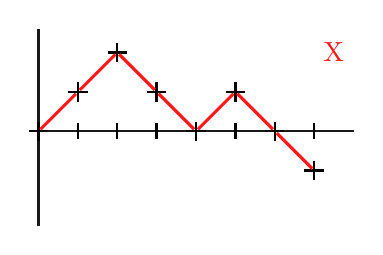
\begin{tikzpicture}
        \tikzset{
          pics/tick/.style args={#1}{code={
            \draw[line width=0.3mm,inner sep=0mm] (0,-#1) -- (0,#1) ;
            },
          }
        }
        \tikzset{
            cross/.pic ={
              \draw[pic actions,rotate=#1,line width=0.3mm]
                (-3.5pt,0) -- (3.5pt,0)
                (0,-3.5pt) -- (0,3.5pt);
            },
          }
        %AXIS Y
        \draw[black!90,line width=0.3mm] (0,-1.2) -- ++(90:2.5cm);
        %AXIS X
        \draw[black!90,line width=0.3mm] (0,0) --++(0:4cm);   

        \foreach \x/\y [count=\i]  in {0/0,0.5/0.5,1/1,1.5/0.5,2/0,2.5/0.5,3/0,3.5/-0.5}{
            \draw[black] (\x,0) pic[rotate=0] {tick={1mm}} ;
            \draw[black] (\x,\y) pic[] {cross={0}} node[inner sep=0mm] (\i) {};
        }
        \draw[red!90,line width=0.4mm] (1)--(2)--(3)--(4)--(5)--(6)--(7)--(8);
        \node[red!90] at (3.75,1) {X};
    \end{tikzpicture} 
\end{center}
\end{figure}
	Then $t\mapsto X_t(\omega)$ is continuous for all $\omega \in \Omega$. The corresponding law $\P^X$ on $C( [0,\infty))$ is called the \textbf{random walk law}, the canonical process under this law is a random walk. It will later be proved that random walk laws of scaled random walks converge weakly on $\mathcal B(C( [0,\infty) ))$ to the Wiener measures, the law of the Brownian motion.
\end{example}
We now turn to the powerful second approach, modifying discontinuous processes into continuous processes.
\subsubsection{The constructing of continuous stochastic processes}
There are different ways of defining the regularity of a real-valued functions. Continuity and differentiability are simple but not very precise notions, a more refined notion is H\"older continuity. 
\begin{ldef}
	\begin{deff}
		A function $f:[0,\infty)\to\R$ is called \textbf{(globally) H\"older continuous} of index $\gamma\in (0,1]$ with constant $K$
		\begin{align*}
			|f(t)-f(s)|\leq K |t-s|^\gamma,\quad \forall t,s\in\R.
		\end{align*}
		We call $f$ \textbf{H\"older continuous on compacts} of index $\gamma\in (0,1]$ with constants $(K_N)_{N\in\N}$ if 
		\begin{align*}
			|f(t)-f(s)|\leq K_N |t-s|^\gamma,\quad \forall t,s\leq N,
		\end{align*}
		for all $N\in \N$. A function $f$ is called \textbf{locally H\"older continuous} of index $\gamma\in (0,1]$ if for all $t$ there is a neighborhood $U_t$ of $t$ and a constant $K_t$ such that 
		\begin{align*}
			|f(t)-f(s)|\leq K_t |t-s|^\gamma,\quad \forall s\in U_t.
		\end{align*}
		Finally, $f$ is called \textbf{H\"older continuous in $t$} of index $\gamma\in (0,1]$ if there is a neighborhood $U_t$ of $t$ in which the previous inequality holds for some constant $K_t$.
	\end{deff}
\end{ldef}
The notion of local and global H\"older continuity is standard, the notion of "{}H\"older continuity on compacts"{} does not exist and is only used here for didactic reasons as it will allow us more easily to talk about tightness on $C([0,\infty))$. The general intuition of H\"older continuity should be that the roughness decreases for increasing $\gamma$ and $\gamma\approx 1$ gives pretty smooth functions. Why is this? Suppose $t$ is close to $s$. Then the difference of the function between $t$ and $s$, also called an increment, is bounded by the distance raised to the power $\gamma$. If $t$ is close to $s$ ($|t-s|<1$) then increasing the power $\gamma$ decreases the size of the increment $|f(t)-f(s)|$, $f$ has infinitesimally small fluctuations (the spikes are not very sharp). The different notions concerning the constant $K$ are secondary for the understanding of roughness (the power $\gamma$ has a stronger effect than the constant $K$) but turn to be very delicate in further applications. \begin{figure}[h]
	\begin{center}
    \begin{tikzpicture}[scale=0.6,transform shape]
        %AXIS Y
        \draw[black!90,line width=0.4mm] (0,-0.6) -- ++(90:2.5cm);
        %AXIS X
        \draw[black!90,line width=0.4mm] (0,0) --++(0:3.5cm);   

        \draw [darkgreen,line width=0.4mm] plot [smooth, tension=0.2] coordinates { (0.2,0.3) (0.4,1) (0.6,0.6) (0.8,0.8) (1,0.4) (1.2,0.5) (1.4,0.7) (1.6,0.4) (1.8,1) (2,0.3) (2.2,1.2) (2.4,0.5)};
    \end{tikzpicture} 
    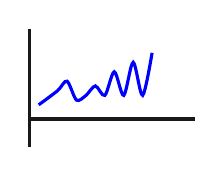
\begin{tikzpicture}[scale=0.6,transform shape]
        %AXIS Y
        \draw[black!90,line width=0.4mm] (0,-0.6) -- ++(90:2.5cm);
        %AXIS X
        \draw[black!90,line width=0.4mm] (0,0) --++(0:3.5cm);   

        % \draw [blue,line width=0.4mm] plot [smooth, tension=0.5] coordinates {(0.2,0.3) (0.4,1.6) (0.6,1) (0.8,1.4) (1,1.1) (1.2,1.4) (1.4,1.25) (1.6,1.3) };
        \draw [blue,line width=0.4mm] plot [smooth, tension=0.5] coordinates { (0.2,0.3) (0.6,0.6) (0.8,0.8) (1,0.4) (1.2,0.5) (1.4,0.7) (1.6,0.5) (1.8,1) (2,0.5) (2.2,1.2) (2.4,0.5) (2.6,1.4)};
    \end{tikzpicture} 
    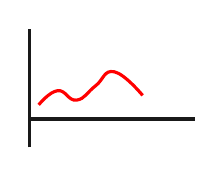
\begin{tikzpicture}[scale=0.6,transform shape]
        %AXIS Y
        \draw[black!90,line width=0.4mm] (0,-0.6) -- ++(90:2.5cm);
        %AXIS X
        \draw[black!90,line width=0.4mm] (0,0) --++(0:3.5cm);   

        % \draw [blue,line width=0.4mm] plot [smooth, tension=0.5] coordinates {(0.2,0.3) (0.4,1.6) (0.6,1) (0.8,1.4) (1,1.1) (1.2,1.4) (1.4,1.25) (1.6,1.3) };
        \draw [red,line width=0.4mm] plot [smooth, tension=0.8] coordinates { (0.2,0.3)  (0.6,0.6)  (1,0.4)  (1.4,0.7)  (1.8,1)   (2.4,0.5)};
    \end{tikzpicture} 
   \caption*{From rough to smooth : small $\gamma$ , medium $\gamma$ , $\gamma=1$}
\end{center}
\end{figure}
	To sharpen your intuition please think about the following exercise.
\begin{luebung}
	\begin{itemize}
		\item $f$ H\"older continuous $\Rightarrow$ $f$ H\"older continuous on compacts $\Rightarrow$ $f$ locally H\"older continuous
		\item If $f$ is (locally) H\"older continuous of index $\gamma$, then $f$ is also (locally) H\"older continuous of index $\gamma'$ for all $\gamma'<\gamma$.
		\item If $f$ is continuously differentiable, then $f$ is H\"older continuous on compacts of index $1$. If $f$ is continuously differentiable with bounded derivative then $f$ is also globally H\"older continuous of index $1$ (which is the same as Lipschitz continuous). Do you have an example?
		\item If $f$ would be H\"older continuous with index $\gamma>1$, then $f$ would be constant (have a look at the differential quotient). That's why we directly restrict to $\gamma\in (0,1]$.
		\item $f(x)=|x|^\beta$, $\beta<1$, is not differentiable at $0$ but locally H\"older continuous of index $\beta$. Away from $0$ they are continuously differentiable, hence, locally Lipschitz continuous.
  	\item Find an example of a function which is continuous but not H\"older continuous for any $\gamma\in (0,1]$. (give it a try and then use google)
	\end{itemize}
\end{luebung}
Motivated by the last example we might think of locally H\"older continuous functions of index $\beta$ to be spiky functions with (possibly many) rough tips that can be as rough as $|x|^\beta$ around $0$. If we think about the graph of $|x|^\beta$ at zero as a piece of metal, would we wipe our hands along the piece? Of course not, only if $\beta \geq 1$. This is how we can picturize roughness in Mathematics, local H\"older continuity is one way of measuring the strength of roughness. Global H\"older continuity allows to additionally estimate increments $|f(t)-f(s)|$ over larger time-horizons, an additional property that does not relate to the spikyness of the graph.
\smallskip

We will prove below that under certain conditions a stochastic process can be "modified"{} in a way that sample paths are continuous. Even better, there is a relatively simple condition under which sample paths are locally H\"older continuous with an identifiable index $\gamma$. Caused by the additional complexity of time there are different notions of equality of stochastic processes that go beyond the uniqueness of the laws when seen as a path-valued random variable. 
\begin{ldef}
	\begin{deff}
		Suppose $X$ and $\tilde X$ are stochastic processes with index set $I$ on the same probability space $(\Omega, \mathcal A, \P)$. Then $\tilde X$ is a \textbf{modification} of $X$ if $\P(X_t=\tilde X_t)=1$ for all $t\in I$. 
	\end{deff}
\end{ldef}
We use the notion $\tilde X$ in order to emphasize that the two stochastic processes are defined on the same probability space. Being modifications of each other is a very different concept of equality of processes than having the same finite-dimensional distributions (i.e. same law). Here, $X$ and $\tilde X$ must be defined on the same probability space and, intersecting events of probability $1$, $X$ and $\tilde X$ automatically have the same finite-dimensional distributions. Thus, in a way, being modifications of each other is much more equal than only having same law. On a path-wise level modifications can be very different. As an example if all $X_t$ are symmetric random variables, then mirroring the path gives processes that look very different but $X$ and $-X$ are modifications of each other. Comparing to random variables there should be an even stronger concept, almost sure equality of the paths. We would like to call two processes indistinguishable if $\P(X_t=\tilde X_t\text{ for all }t\in I)=1$. But there is a technical problem: Writing $\{X_t=\tilde X_t\text{ for all }t\in I\}=\cap_{t\in I}\{X_t=\tilde X_t\}$ there is again an uncountability issue. The righthand side is measurable if $I$ is countable, but not necessarily if $I$ is uncountable. Here is the good definition:
\begin{ldef}
	\begin{deff}
		Suppose $X$ and $\tilde X$ are stochastic processes with index set $I$ on the same probability space $(\Omega, \mathcal A, \P)$. Then $X$ and $\tilde X$ are called \textbf{indistinguishable} if there is an event $C$ with probability $1$ such that $X_t(\omega)=\tilde X_t(\omega)$, $t\in I,$ for all $\omega\in C$.
	\end{deff}
\end{ldef}
Here is the simplest example to separate both notions of equality for processes. Suppose $\mathcal U\sim \mathcal U([0,1])$ is a uniformly distributed random variable on some probability space $(\Omega, \mathcal A, \P)$ and define the stochastic processes $X_t:=0$ and $\tilde X_t:=\mathbf 1_{\{U\}}(t)$ on $(\Omega, \mathcal A, \P)$ with index set $I=[0,1]$. Then $\tilde X$ is a modification of $X$ as $\P(X_t=\tilde X_t)=\P(U\neq t)=1$ but their paths are almost surely different (see the drawing). 
\begin{figure}
	\begin{center}
	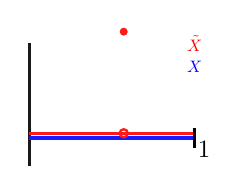
\begin{tikzpicture}[scale=0.6,transform shape]
        \tikzset{
          pics/tick/.style args={#1}{code={
            \draw[line width=0.4mm,inner sep=0mm] (0,-#1) -- (0,#1) ;
            },
          }
        }
        %AXIS Y
        \draw[black!90,line width=0.4mm] (0,-0.6) -- ++(90:2.6cm);
        %AXIS X
        \draw[blue!90,line width=0.4mm] (0,0) --++(0:3.5cm);   
        \draw[red!90,line width=0.4mm] (0,0.1) --++(0:3.5cm);
        \draw[black] (3.5,0) pic[] {tick={6pt}} node[yshift=-2.5mm,xshift=2mm,scale=1.5] {1};
        \node[circle,inner sep=0.6mm,fill opacity=0,draw=red!90,line width=0.3mm] at (2,0.1) {};
        \node[circle,inner sep=0.6mm,fill=red!90] at (2,2.25) {};

        \node[blue] at (3.5,1.5) {$X$};
        \node[red] at (3.5,2) {$\tilde X$};
    \end{tikzpicture}  
    \caption*{modifications but not indistinguishable}
\end{center}
\end{figure}
The next exercise is useful to play with the definition.
	\begin{luebung}
	\begin{itemize}
			\item
			Show that (i)$\Rightarrow$(ii)$\Rightarrow$(iii) hold, for
		\begin{enumerate}[label=(\roman*)]
			\item $X$ and $\tilde X$ are indistinguishable.
			\item $X$ is a modification of $\tilde X$.
			\item $X$ and $\tilde X$ have the same finite-dimensional distributions (and same law).
		\end{enumerate}
		Give examples that the converses are generally wrong.
		\item If $X$ is almost surely continuous, then setting $X(\omega)\equiv 0$ for all $\omega\notin C$ gives a modification with continuous sample paths.
		\item If $X$ is almost surely continuous, then every almost surey continuous modification $\tilde X$ is indistinguishable from $X$ ($\Q$ being dense in $\R$ is always useful for continuous functions)
	\end{itemize}
\end{luebung}
In order to construct continuous processes from processes with unknown path regularity we will refer to the famous Kolmogorov-Chentsov theorem. The theorem is actually much better, under a H\"older-type condition (which is easy to check in many situations) a modification with locally H\"older continuous paths is constructed.
\begin{lAussageWerkzeug}
\begin{theorem}[Kolmogorov-Chentsov theorem]\label{thm:chentsov}
	Suppose $(X_t)_{t\geq 0}$ is a stochastic process on $(\Omega,\cA,\mathbb{P})$ such that for all $T>0$ there are $c, \alpha$, $\beta$ with
	\begin{align*}
		\E\big[\lvert X_t - X_s \rvert^{\alpha}\big] \leq c \cdot \lvert t - s \rvert^{1+\beta},\quad \forall t,s \leq T.
	\end{align*}
	Then there is a modification $\tilde X$ of $X$ such that $\tilde X$ has locally H\"older continuous (in particular continuous) paths of order $\gamma$ for all $\gamma<\frac{\beta}{\alpha}$.
\end{theorem}
\end{lAussageWerkzeug}
\begin{proof}[Proof]
	We do not prove the probability of H\"older continuity is $1$ for the modification (this is not necessarily a measurable event!) but following the proof closely we will construct explicitly a measurable set $A\in \mathcal A$ of probability $1$ on which the modification is continuous. \smallskip

	Let us fix $\gamma<\frac{\beta}{\alpha}$, set $K := \frac{2}{1-2^{-\gamma}}$ and assume the index set is $[0,1]$, the extension to $[0,\infty)$ is discussed in the very end of the proof. We will construct a set $A\in \cA$ of measure $1$ such that $\omega \mapsto X_t(\omega)$ is (locally) H\"older continuous with constant $K$ and index $\gamma$ when restricted to a set $\mathcal D$ of time-points which is dense in $[0,1]$.  Then we redefine $X_t(\omega)$ for $t\notin \mathcal D$ as right-limits from $\mathcal D$ for $\omega \in A$ and $X(\omega)\equiv 0$ for $\omega \notin A$. The set $\mathcal D$ of good time-points will be the set of all dyadics in $[0,1]$, defined as follows: $\cD_n = \{ 0, \frac{1}{2^n},\frac{2}{2^n},...,1\}$ and $\cD \coloneqq \bigcup_{n=1}^{\infty} \cD_n$. Note that $\mathcal D_1\subseteq\cD_2\subseteq ... \subseteq \cD$ and $\cD$ is dense in $[0,1]$.
	\begin{figure}[h]
		\begin{center}
			\includegraphics[scale=0.07]{dyadic1.jpeg}
			\caption*{approximation on the dyadics}
		\end{center}
		\end{figure}
		The main step is to use the assumption to prove the H\"older property on the diadics.
		\begin{lstep}
			$X$ almost surely satisfies the H\"older property on $\mathcal D$.
		\end{lstep}
	The argument goes as follows: We prove the almost sure H\"older continuity on $\cD$ by chaining from one dyadic to another by a shortest path along neighboring dyadic points. Such increments are first estimated by Markov's inequality to obtain an almost sure uniform upper bound through the Borel-Cantelli lemma. \smallskip

	(i) In a first step let us estimate increments over neighboring dyadic numbers in $\mathcal D_n$ by combining the Markov inequality and Borel-Cantelli. This step will provide the almost sure event $A$. First note that 
			\begin{align}\label{P}
				\mathbb{P}\left(\lvert X_t - X_s \rvert > \varepsilon \right) \overset{\text{Markov}}{\leq}  \frac{\E\left[ \lvert X_t - X_s \rvert^{\alpha} \right]}{\varepsilon^{\alpha}} \overset{\text{ass.}}{\leq} c  \frac{\lvert t -s \rvert^{1+\beta}}{\varepsilon^{\alpha}}
			\end{align}
			so that, in particular,
			\begin{align*}
				\mathbb{P}\big(| X_{\frac{k}{2^n}} - X_{\frac{k-1}{2^n}}| > 2^{-\gamma  n}\big) 
				\leq c  2^{\alpha \gamma n} \cdot 2^{-n(1+\beta)} 
				= c  2^{-n (1+\beta - \alpha \gamma)}.
			\end{align*}
			Since a maximum is larger than a given number if each element of the maximum is larger than that given number, we obtain
			\begin{align*}
				\mathbb{P} \big( \underbrace{\max_{k\leq 2^n} \lvert X_{\frac{k}{2^n}} - X_{\frac{k-1}{2^n}} \rvert > 2^{-\gamma  n}}_{=:A_n} \big) 
				&\leq \mathbb{P} \Big( \bigcup_{k=1}^{2^n} \big\{ \big\lvert X_{\frac{k}{2^n}} - X_{\frac{k-1}{2^n}}\big\rvert \geq 2^{-\gamma  n}\big\}\Big) \\
				\overset{\text{sub. add.}}&{\leq} \sum_{k=1}^{2^n} \mathbb{P}\big( \lvert X_{\frac{k}{2^n}} - X_{\frac{k-1}{2^n}}\big\rvert \geq 2^{-\gamma \cdot n}\big) \\
				&\leq c \cdot \sum_{k=1}^{2^n} 2^{-n (1+\beta - \alpha \gamma)} \\
				&= c \cdot 2^{-n(\beta - \alpha  \gamma)}.
			\end{align*}
			The righthand side is summable by the choice of $\gamma$. Hence, Borel-Cantelli \ref{BC} implies that $\limsup A_n$ is a zero set. Defining $A:= \{ A_n \text{ i.o.}\}^c \in \cA$ then yields $\mathbb{P}(A)=1$, and that, for all $\omega \in A$, there are numbers $n_0(\omega)$ so that
			\begin{align}\label{kolmogorov_tight_eq1}
				\max_{k\leq 2^n} \big\lvert X_{\frac{k}{2^n}} - X_{\frac{k-1}{2^n}}\big\rvert \leq \frac{1}{2^{\gamma  n}}, \quad \forall n \geq n_0(\omega).
			\end{align}
			The important point is that on $A$ we can estimate \underline{all} increments over neighboring dyadics.\smallskip
		
		(ii) The next step is the so-called chaining ("hangeln") trick. Using the above estimate for increments over neighboring dyadics we can chain cleverly from one dyadic to another by going only over neighboring dyadics of same type. In fact, chaining all the way along neighbors is a mess writing, an induction by chaining through coarser $\mathcal D_k$ is simpler to write (see the picture).
		\begin{figure}[h]
			\begin{center}
				\includegraphics[scale=0.07]{dyadic2.jpeg}
				\caption*{chaining trick (orange is subset of blue)}
			\end{center}
			\end{figure}
		
		Fix $\omega \in A$ so that we can use \eqref{kolmogorov_tight_eq1} for all $m\geq N \geq n_0(\omega)$. Now suppose $m > N$ and $t,s\in \cD_m$ are close enough such that $|t- s| < \frac{1}{2^N}$. We use induction (starting at $m=N+1$) to prove that
		\begin{align*}
			| X_t(\omega) - X_s(\omega) | \leq 2  \sum_{k=N+1}^m \frac{1}{2^{\gamma k}},\quad \forall m>N,
		\end{align*}
holds.
		\begin{itemize}
				\item Induction starts at $m=N+1$: For $m=N+1$, $t$ and $s$ must be neighbors as the distance between time-points in $\mathcal D_{N+1}$ is precisely $\frac{1}{2^{N+1}}<\frac{1}{2^N}$ if $t$ and $s$ are neighbors and otherwise larger than $\frac{1}{2^N}$. Hence, the claim follows from \eqref{kolmogorov_tight_eq1} as $m\geq n_0(\omega)$.
				\item Induction step: Now suppose the claim holds for some $m-1>N$ and take $s,t\in \cD_m$. We chose $t^{\prime},s^{\prime}\in\cD_{m-1}$ as in the picture (the closest ones between $t$ and $s$), use the estimate on increments for neighbors (note that $\mathcal D_{m-1}\subseteq \mathcal D_{m}$) and the induction hypothesis:
					\begin{align*}
						\lvert X_t(\omega) - X_s(\omega)\rvert
						%\overset{m \geq N \geq n_0(\omega)}
						\overset{\Delta}&{\leq} \lvert X_t(\omega) - X_{t^{\prime}}(\omega) \rvert + \lvert X_{t^{\prime}}(\omega) - X_{s^{\prime}}(\omega) \rvert + \lvert X_{s^{\prime}} - X_s(\omega) \rvert \\
						\overset{\text{2x }\eqref{kolmogorov_tight_eq1},\text{ Ind. hyp.}}&{\leq}   \frac{1}{2^{\gamma m}} + 2  \sum_{k=N+1}^{m-1} \frac{1}{2^{\gamma  k}} +   \frac{1}{2^{\gamma m}} \\
						&= 2  \sum_{k=N+1}^{m} \frac{1}{2^{\gamma  k}}
					\end{align*}
			\end{itemize}
		(iii) We can now show that $t\mapsto X_t(\omega)$ satisfies the local H\"older continuity with constant $K$ on $\mathcal D$ for all $\omega \in A$.	
		To do so fix some $t\in\mathcal D$ and define the neighborhood $U_t(\omega)=(t-h(\omega), t+h(\omega))$ with $h(\omega) = 2^{-n_0(\omega)}$. If $s\in U_t(\omega)$, then there is some $N\geq n_0(\omega)$ with $\frac{1}{2^{N+1}} \leq \lvert t - s \rvert \leq \frac{1}{2^N}$, so that, from the above,
			\begin{align}\label{cau}
				\lvert X_t(\omega) - X_s(\omega) \rvert \overset{\text{(ii)}}{\leq} 2  \sum_{k=N+1}^{\infty} \frac{1}{2^{\gamma  k}} = \frac{1}{2^{\gamma(N+1)}} \sum_{k=0}^{\infty} \frac{2}{2^{\gamma  k}} \leq \underbrace{K}_{=\frac{2}{1-\frac{1}{2^{\gamma}}}}  \lvert t-s \rvert^{\gamma}.
			\end{align}
			Hence, restricted to the time-points in $\mathcal D$, $t\mapsto X_t(\omega)$ is locally H\"older continuous with index $\gamma$ for all $\omega \in C$.\smallskip
			
			Carrying out the same construction on all intervals $[n,n+1]$ and intersecting the appearing events $A_n$ gives an event (denoted by $A$ again) of probability $1$ on which the above holds for a dense subset (also denoted by $\mathcal D$ again) of $[0,\infty)$ 
\begin{lstep}
	Defining the H\"older continuous modification $\tilde X$.
\end{lstep}
 Fix $t\notin \mathcal D$ and take any sequence $(s_n)$ in $\mathcal D$ that decreases to $t$. By \eqref{cau}, for all $\omega\in A$ the sequence $(X_{s_n}(\omega))_{n\in \N}$ is a real Cauchy sequence, hence, converges. Note that \eqref{cau} also shows that the limit is independent of the choice of the sequence. Now we define
		\begin{align*}
			\tilde X_t(\omega)=
			\begin{cases}
				\lim_{s\to t, s\in \cD}X_{s}(\omega)&: t\notin \mathcal D\\
				X_t(\omega)&:  t\in \mathcal D
			\end{cases}, \quad t\geq 0,
		\end{align*}
		for $\omega \in A$ and $\tilde X(\omega)\equiv 0$ for $\omega\notin A$. Then
		\begin{itemize}
			\item $\tilde X$ is a stochastic process on $(\Omega, \mathcal A, \P)$ because all $\tilde X_t$ are random variables on $(\Omega, \mathcal A, \P)$ as measurability is preserved under taking limits.
			\item for all $\omega \in A$, $t\mapsto \tilde X(\omega)$ inherits the local H\"older continuity of index $\gamma$ as $|\cdot|$ is continuous, for $\omega \notin A$ the H\"older continuity is trivial (zero-function).
		\end{itemize}
		It only remains to show that $\tilde X$ is a modification of $X$. For $t\in \mathcal D$ we have $\P(X_t=\tilde X_t)\geq \P(A)=1$. For $t\notin \mathcal D$ we use that \eqref{P} implies  $X_s\overset{P}{\to} X_t$, $s\to t$. Additionally, by definition of $\tilde X$, $X_s$ converges along $\mathcal D$ almost surely to $\tilde X_t$ (on the event $A$), hence, in particular $X_s\overset{P}{\to} \tilde X_t$ as $s\to t$. Since limits under the convergence in probability are almost surely unique this also shows that $\P(X_t=\tilde X_t)=1$ for $t\notin \mathcal D$. That's it, $\tilde X$ is a modification of $X$ with H\"older continuous paths.
\end{proof}
Please keep in mind the construction of the modification $\tilde X$. Away from some zero probability event the modification just consists of the old paths extended continuously from a dense subset of time, which for continuous paths does not change anything at all.
\begin{laufmerksamkeit}
	If $X$ has continuous paths then $\tilde X$ and $X$ are indistinguishable, $\tilde X$ only differs on a zero set where it is set to the zero function. In that case Kolmogorov-Chentsov should  rather be seen as a statement on the H\"older-regularity of paths of $X$.
\end{laufmerksamkeit}
There is a simple example which shows best how things work. Returning to the zero process $X$ on $[0,1]$ and the random one-point process $Y=\mathbf 1_{\{U\}}$ from above, then $Y$ is discontinuous and $X$ is an almost surely continuous modification of $Y$. 
\begin{luebung}
	Go through the construction of the proof for $Y=\mathbf 1_{\{U\}}$ and check why the modification $\tilde Y$ from the proof is indistinguishable from the trivial zero process. Can you identify the occurring events of probability $1$? \smallskip
\end{luebung}
Let us now summarize the section for the Kolmogorov-Chentsov approach of constructing continuous stochastic processes with given finite-dimensional marginals:
\begin{lWarnhinweis}
	\begin{enumerate}[label=(\roman*)]
		\item Write down a consistent family $\{\P_J:|J|<\infty\}$ of finite-dimensional measures indexed by $I$.
		\item Use Theorem \ref{KolmogorovProcess} to obtain a stochastic process $X$ on some $(\Omega, \mathcal A, \P)$ with finite-dimensional marginals $\P_J$.
		\item Check the H\"older-type condition of Kolmogorov-Chentsov to obtain a continuous (even H\"older continuous) modification $\tilde X$. Since modifications have the same finite-dimensional marginals, $\tilde X$ has the finite-dimensional marginals $\P_J$. 
		\end{enumerate}
		If of interest, use the law $\P^{\tilde X,c}$ of $\tilde X$ induced on $\mathcal B(C([0,\infty)))$ with finite-dimensional marginals $\P_J$ and work with the canonical construction.
	\end{lWarnhinweis}
	There is a large class of processes for which the approach can be applied easily. Centered Gaussian processes are natural candidates as we already know how to construct from the covariance function $K$ a family of consistent finite-dimensional distributions. Since linear combinations of Gaussian vectors are Gaussian, expectations of powers of $|X_t-X_s|$ can be computed as a lot is known for moments of normal distributions. In the next section the approach will be carried out for the Brownian motion.

\section{Foundation of Brownian motion}
\marginpar{\textcolor{red}{Lecture 23}}
We now come to the big final of this set of lectures notes. The Brownian motion. While the origin was to describe the two-dimensional movement of pollen in water by the biologist Robert Brown in 1827 \footnote{Brown, Robert: "{}A brief account of microscopical observations made in the months of June, July and August, on the particles contained in the pollen of plants; and on the general existence of active molecules in organic and inorganic bodies"{}, Philosophical Magazine, 4 (21), 1828, 161–173.} the first rigorous formulations date back to the beginning of the last century. The wide use of Brownian motion is perhaps best reflected in citing more applications in Einstein's treatment of the movement of molecules \footnote{Einstein, Albert: "{}Investigations on the Theory of Brownian Movement"{}, 1956, New York: Dover.} and Bachelier's famous model of a stock in his \enquote{Th\'{e}orie de la speculation} \footnote{Bachelier, Louis: "{}Th\'eorie de la sp\'eculation"{}, Annales Scientifiques de l'École Normale Supérieure, 3 (17), 1900, 21–86.}. Also within Mathematics the Brownian motion and it's generalizations have turned out to be universal objects that appear very naturally when discrete structures are made to converge to continuous structures. The aim of this section is to present the foundations and to prove the universal approximation property of a Brownian motion in the simplest setting of stochastic processes. 
\begin{ldef}
\begin{deff}\label{def_BM}
	A real-valued stochastic process $(B_t)_{t\geq 0}$ on some probability space $(\Omega,\cA,\mathbb{P})$ is called a \textbf{(standard) Brownian motion} if
	\begin{enumerate}[label=(\roman*)]
		\item $B_0 = 0$ $\P$-almost surely
		\item $B$ has \textbf{\smash{stationary and independent increments}}, i.e. 
			\begin{itemize}
				\item
				the distribution of $B_{t+h}-B_t$ depends on $h$ but not on $t$,
				\item
				the increments	$B_{t_1} - B_{t_0},...,B_{t_n} - B_{t_{n-1}}$ are independent random variables for all $0 \leq t_0 \leq ...\leq t_n$.
			\end{itemize}
		\item
			The paths $t \mapsto B_t$ are $\P$-almost surely continuous.
		\item
			$B_t \sim \cN(0,t)$ for all $t > 0$
	\end{enumerate}
	Typically one also calls $\sigma B$ a Brownian motion if $B$ is a standard Brownian motion and $\sigma>0$. If $B_1,...,B_d$ are independent Brownian motions on the same probability space $(\Omega, \mathcal A, \P)$, then $B:=(B_1,...,B_d)$ is called a \textbf{$d$-dimensional Brownian motion}.
\end{deff}
\end{ldef}
\begin{figure}[h]
	\begin{center}
		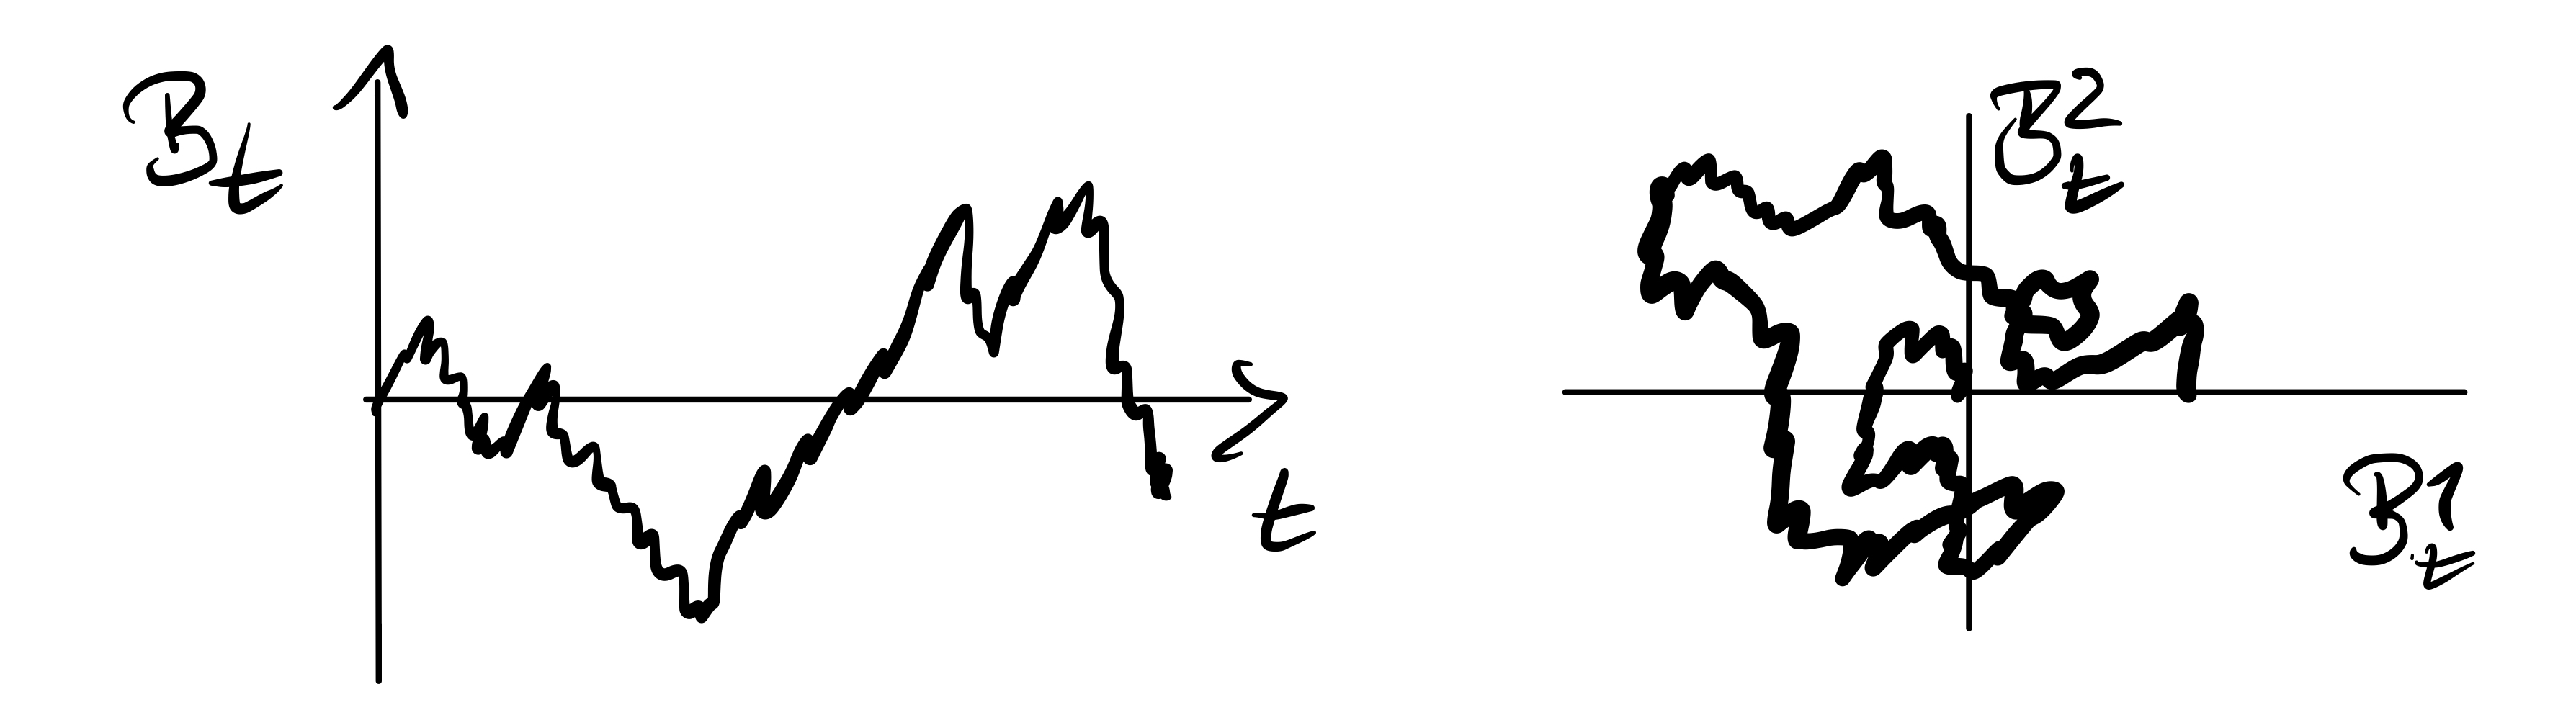
\includegraphics[scale=0.08]{BB.jpeg}
		\caption*{Visualisation of one- and two-dimensional Brownian motions}
	\end{center}
\end{figure}	
There are other equivalent definitions of the Brownian motion, viewing the Brownian motion as special case of two of the most important classes of stochastic processes. 
\begin{itemize}
	\item A Brownian motion is an almost surely continuous \textbf{centered Gaussian process} indexed by $[0,\infty)$ with covariance function $K(s,t)=s\wedge t$. 
	\item A \textbf{L\'evy process} is a stochastic process with sample paths that are right continuous with left limits (RCLL) that start in $0$ and have stationary and independent increments. A Brownian motion is the only non-deterministic L\'evy process with continuous sample paths. 
\end{itemize}
We are not going deeper into the rich class of L\'evy processes which is typically seen as the continuous-time and -space generalization of random walks since random walks satisfy the same independence and stationarity property of increments. At least it should be mentioned that the Poisson process and a useful generalisation share the L\'evy property of the Brownian motion:
\begin{example}
	Suppose $Y_1,...$ is an iid sequence and $N$ is a Poisson process (see Example \ref{ex:sp}) that is independent of the sequnce. Then 
	\begin{align*}
			X_t:=\sum_{k=1}^{N_t}Y_k,\quad t\geq 0,
	\end{align*}
	is called \textbf{compound Poisson process}.
\end{example}
A compound Poisson process is the natural generalisation of a Poisson process, the jumps at the jump-times of the Poisson process are allowed to be random instead of $1$. It is actually not so easy to show that the Poisson process is a L\'evy process. But if we take that for granted it is a good (but not simple) exercise to compute with characteristic functions to infer that also all compound Poisson processes are L\'evy processes.
\begin{luebung}
	Show that the compound Poisson process is a L\'evy process.
\end{luebung}
There is a complete description of all stochastic processes that satify the L\'evy property. All L\'evy processes are sums of a deterministic linear drift, a Brownian motion, and a limit of compound Poisson processes in which the jump frequency is increased (not easy!). Adding a linear drift to a compound Poisson process with negative jumps $X_t=a\cdot t+\sum_{k=i}^{N_t}Y_k$ is a simple model for the wealth of an insurance compancy. The drift represents the deterministic income through the insurance premium of customers, the negative jumps represent the costs of claims. In Insurance Mathematics the model is called \textbf{Cram\'er-Lundberg model}.
\begin{figure}[h]
	\begin{center}
		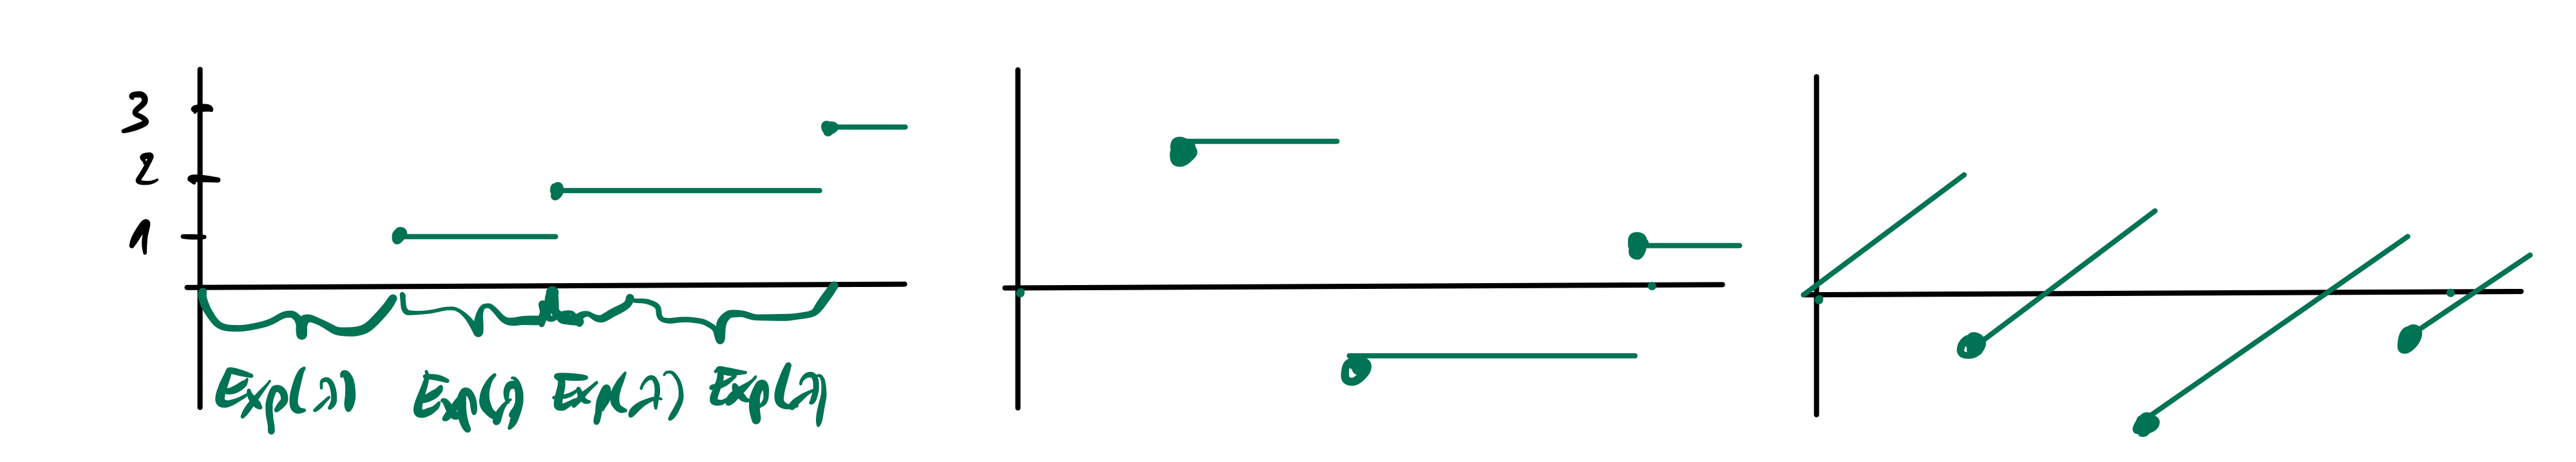
\includegraphics[scale=0.1]{Levy.jpeg}
		\caption*{Poissonprocess, compound Poisson process, Cram\'er-Lundberg model}
	\end{center}
\end{figure}

Instead of working with the L\'evy point of view we use the Gaussian point of view and first prove the above claimed connection:
\begin{laussagewerkzeug}
	\begin{prop}\label{BMGaussian}
		A real-valued stochastic process $X$ on $(\Omega, \mathcal A, \P)$ with index-set $I=[0,\infty)$ is a Brownian motion if and only if $X$ is a centered Gaussian process with covariance function $K(s,t)=s\wedge t$ and almost surely continuous sample paths.
	\end{prop}
\end{laussagewerkzeug}
\begin{proof}[Proof]
	"$\Rightarrow$"{}: Let $s<t$. First note that the increments $X_t-X_s$ are $\mathcal N(0,t-s)$ by combining properties (i), (ii), and (iii) since $X_{t}-X_s\sim X_{t-s}-X_0\sim X_{t-s}\sim \mathcal N(0,t-s)$. Writing 
	\begin{align*}
		\left({X_s}\atop {X_t}\right)=\left({X_s}\atop{X_s+(X_t-X_s)}\right)=A\cdot \left({X_s}\atop{ X_{t}-X_s}\right)
	\end{align*}
	with $A=\left(\begin{matrix}
		1 & 0 \\
		1 & 1 
		\end{matrix}\right)$ shows that $(X_s,X_t)$ is a Gaussian vector as $(X_t, X_{t}-X_s)$ is a vector of independent Gaussian random variables. The same trick works for all finite-dimensional distributions $(X_{t_1},...,X_{t_k})$ which can be written as a matrix multiplication of some (more complicated) matrix with a vector of increments which are independent and Gaussian. This shows that $X$ is a Gaussian process. Furthermore, as $X_t\sim \mathcal N(0,t)$ the Gaussian process is also centered. To compute the covariance function $K(s,t)$ we proceed similarly:
		\begin{align*}
			\varphi_{(X_s,X_t)}(t_1,t_2) &= \E \big[ \exp\big(i(t_1 X_{s}+t_2 X_{t})\big)\big] \\
				&= \E \big[ \exp\big(i(t_1+t_2)X_{s}\big)\exp \big(i  t_2  (X_{t}-X_{s}) \big)\big] \\
				\overset{\text{ind. incr.}}&{=} \E \big[ \exp\big(i(t_1+t_2)X_{s}\big)\big]\E\big[\exp \big(i  t_2  (X_{t}-X_{s}) \big)\big] \\
				\overset{\text{centr. Gaussian}}&{=}\exp\Big(-\frac{1}{2}(t_1+t_2)^2s\Big)\exp\Big(-\frac{1}{2}t_2^2(t-s)\Big)\\
					&= \exp\bigg( -\frac{1}{2} \bigg\langle \begin{pmatrix}
						t_1 \\
						t_2
					\end{pmatrix},\begin{pmatrix}
					s & s \\
					s & t
				\end{pmatrix}\cdot \begin{pmatrix}
				t_1 \\
				t_2
			\end{pmatrix} \bigg\rangle \bigg),
		\end{align*} 
		which is the characteristic function of a $\cN \bigg( \begin{pmatrix}
			0\\
			0
		\end{pmatrix}, \begin{pmatrix}
		s & s \\
		s & t
	\end{pmatrix}\bigg)$ random vector. Since the characteristic function characterises the law it follows that $K(s,t)=s\wedge t$.\smallskip

	"$\Leftarrow$"{}: We check the three defining properties of a Brownian motion:

	(i) $\text{Var}[X_0]=\text{Cov}(X_0,X_0)=0\wedge 0=0$, hence, $X_0=0$ almost surely.\smallskip
	
	(ii) The assumption implies that the finite-dimensional marginals $(X_{t_1},...,X_{t_k})$ are centered Gaussian vectors. Writing the vector of increments $(X_{t_2}-X_{t_{1}},...,X_{t_k}-X_{t_{k-1}})$ as a matrix multiplication of $(X_{t_1},...,X_{t_k})$ shows that the vector of increments is centered Gaussian, hence, is uniquely determined by all  covariances according to the discussion at the end of Chapter \ref{chapter:CV}. To show that all covariances are zero we use linearity of expectations. For $t_i\geq t_{i-1}\geq t_j\geq t_{j-1}$ this gives
	\begin{align*}
		&\quad \text{Cov}(X_{t_j}-X_{t_{j-1}}, X_{t_i}-X_{t_{i-1}})\\
		&=\text{Cov}(X_{t_j},X_{t_{i}}) -\text{Cov}(X_{t_{j-1}},X_{t_{i}})+\text{Cov}(X_{t_{j-1}},X_{t_{i-1}})-\text{Cov}(X_{t_{j}},X_{t_{i-1}})\\
		&=t_j-t_{j-1}+t_{j-1}-t_j=0.
	\end{align*}
	Hence, the covariance matrix is a diagonal matrix and thus the increments are independent. Since $(X_t,X_{t+h})$ is a Gaussian vector also the linear combination $X_{t+h}-X_{t}$ is Gaussian. The variance can be computed from the assumed variance structure:
	\begin{align*}
		\text{Var}[X_{t+h}-X_t]=\text{Var}[X_{t+h}]-2\text{Cov}(X_{t+h},X_t)-\text{Var}[X_t]=(t+h)-2t+t=h,
	\end{align*}
	which is independent of $t$.\smallskip

	(iii) The continuous sample paths have been assumed.\smallskip

	(iv) Follows from the assumed covariance function for $t=s$.
\end{proof}
Suppose $B$ is a Brownian motion for which $t\mapsto B_t(\omega)$ is continuous for all $\omega\in C$ for some event $C$ of probability $1$. Defining $\tilde B(\omega)=B(\omega)$ for $\omega \in C$ and $\tilde B(\omega)\equiv 0$ for $\omega\notin C$ yields a continuous modification of $B$. Since modifications have the same finite-dimensional marginals, also $\tilde B$ is a centered Gaussian process with covariance function $K(s,t)=t\wedge s$, hence, a Brownian motion. The induced law on $\mathcal B(C([0,\infty)))$ is called the \textbf{Wiener measure} and the canonical process on the canonical space with the Wiener measure is a Brownian motion. If useful we can always assume that $\omega\mapsto B_t(\omega)$ is continuous for all $\omega\in \Omega$ and use the  explicite canonical probability space. As an example, this will always be done if quantities like $Y=\sup_{t\in [0,1]}B_t$ are involved as rewriting them as $Y=\sup_{t\in[0,1]\cap \Q} B_t$ makes them random variables on probability spaces on which the Brownian motion is continuous for all $\omega$.\smallskip

Before continuing to discuss any properties let us prove the existence of a Brownian motion.  
\begin{lsuperwichtigersatzExistence}
\begin{theorem}\label{canonical_construction_BM}
	There is a probability space $(\Omega,\cA,\mathbb{P})$ and a stochastic process $(X_t)_{t\geq 0}$ on $(\Omega,\cA,\mathbb{P})$ that satisfies the properties of a Brownian motion. In other words: Brownian motion exists.
\end{theorem}
\end{lsuperwichtigersatzExistence}
\begin{proof}[Proof]
The proof uses the abstract Kolmogorov theory of the previous section in combination with the previous proposition.
\begin{lstep}
	There is a centered Gaussian process $X$ indexed by $I=[0,\infty)$ with covariance function $K(s,t)=s\wedge t$.
\end{lstep}
	This follows from Kolmogorov's extension theorem for Gaussian processes with the symmetric positive semidefinite function $K(t,s)=s\wedge t$.
\begin{lstep}
	There is a modification $B$ of $X$ with continuous sample paths.
\end{lstep}
We have seen in the previous proof how the covariance structure implies $X_t-X_s\sim \mathcal N(0,t-s)$. Since $\E[X^4]=3 \sigma^2$ for $X\sim \mathcal N(0,\sigma^2)$ the situation fits perfectly to the Kolmogorov-Chentsov theorem with $\alpha=4$, $\beta=1$, and $K=3$, even with equality:
	\begin{align*}
		\E\big[|X_t-X_s|^{4}\big]=3|t-s|^{1+1}.
	\end{align*}
But then $X$ has a modification $B$ with continuous (even H\"older continuous with index $\gamma<\frac{1}{4}$) sample paths. As a modification $B$ has the same finite-dimensional marginals as $X$. Hence, $B$ is a centered Gaussian process with covariance function $K(t,s)=s\wedge t$. Since $B$ has continuous samples paths the theorem follows from Proposition \ref{BMGaussian}.
\end{proof}
There are many other constructions of the Brownian motion, some of them are more instructive than the proof given above. Nonetheless, there are good reasons to go through the abstract approach. First, the Kolmogorov extension theorem is also important for many other contexts (such as constructing iid sequences, other Gaussian processes, Markov processes), secondly, the Kolmogorov-Chentsov chaining argument would be needed anyways to derive a tightness criterion for the proof of Donsker's theorem (compare Theorem \ref{thm:KolTightness} below). To get an impression, here is the sketch of one alternative proof:
\begin{proof}[Sketch of L\'evy's construction of the Brownian motion]
	The Brownian motion will only be constructed on $[0,1]$, sticking together an iid sequence of Brownian motions on $[0,1]$ then gives a Brownian motion on $[0,\infty)$.
	\begin{figure}[h]
		\begin{center}
			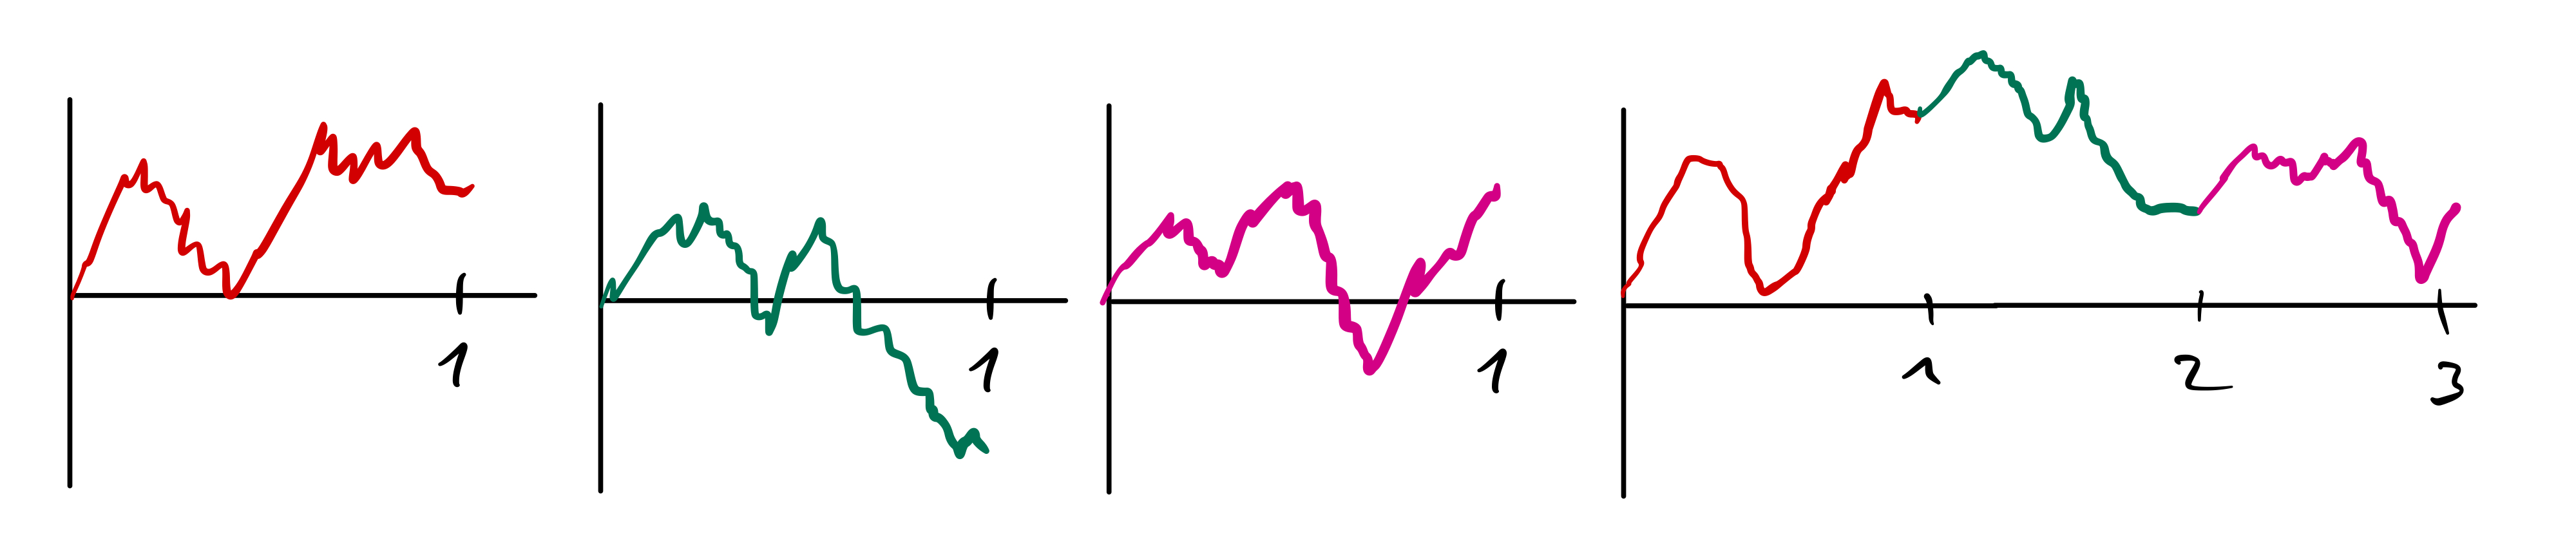
\includegraphics[scale=0.08]{BML1.jpeg}
		\end{center}
	\end{figure}	

	The trick is to construct a sequence of "discrete"{} Brownian motions on the dyadic numbers $\mathcal D_1\subseteq \mathcal D_2\subseteq \cdots$ in a consistent way, such that the values on $\mathcal D_n$ are equal to the values in $\mathcal D_m$ for all $n>m$. With a discrete Brownian motion we mean a process indexed by $\mathcal D_m$ which satisfies the properties of a Brownian motion for values from $\mathcal D_m$. Suppose $(Z_d)_{d\in \mathcal D}$ is an iid sequence ($\mathcal D$ is countable) of $\mathcal N(0,1)$ random variables. The sequence and the probability space exist due to the Kolmogorov extension theorem. The discrete Brownian motions indexed by $\mathcal D_m$ are defined inductively: 
	\begin{itemize}
		\item $B^{(m)}_0 = 0$, $B^{(m)}_1 = Z_1$
		\item Suppose that $B^{(m-1)}$ was already defined on $\cD_{m-1}$. Then define $B^{(m)}$ on $\mathcal D_m$ as
		\begin{align*}
			B^{(m)}_d =\begin{cases}
				B^{(m-1)}_d&: d\in \mathcal D_{m-1}\\
				 \frac{1}{2}\big(B^{(m-1)}_{d-2^{-m}} +B^{(m-1)}_{d+2^{-m}}\big) +  2^{-\frac{(m+1)}{2}}\cdot Z_d&: d\in \mathcal D_m\backslash D_{m-1}
			\end{cases},
		\end{align*}
	\end{itemize}
	that is to keep the old values on $\mathcal D_{m-1}$ and to add to the linear interpolation at the new dyadics $\mathcal D_{m}\backslash \mathcal D_{m-1}$ an independent $\mathcal N(0,2^{-(m+1)})$ random variable. The construction is best understood in the picture, in which the $B^{(m)}$ have been interpolated linearly.
	\begin{figure}[h]
		\begin{center}
			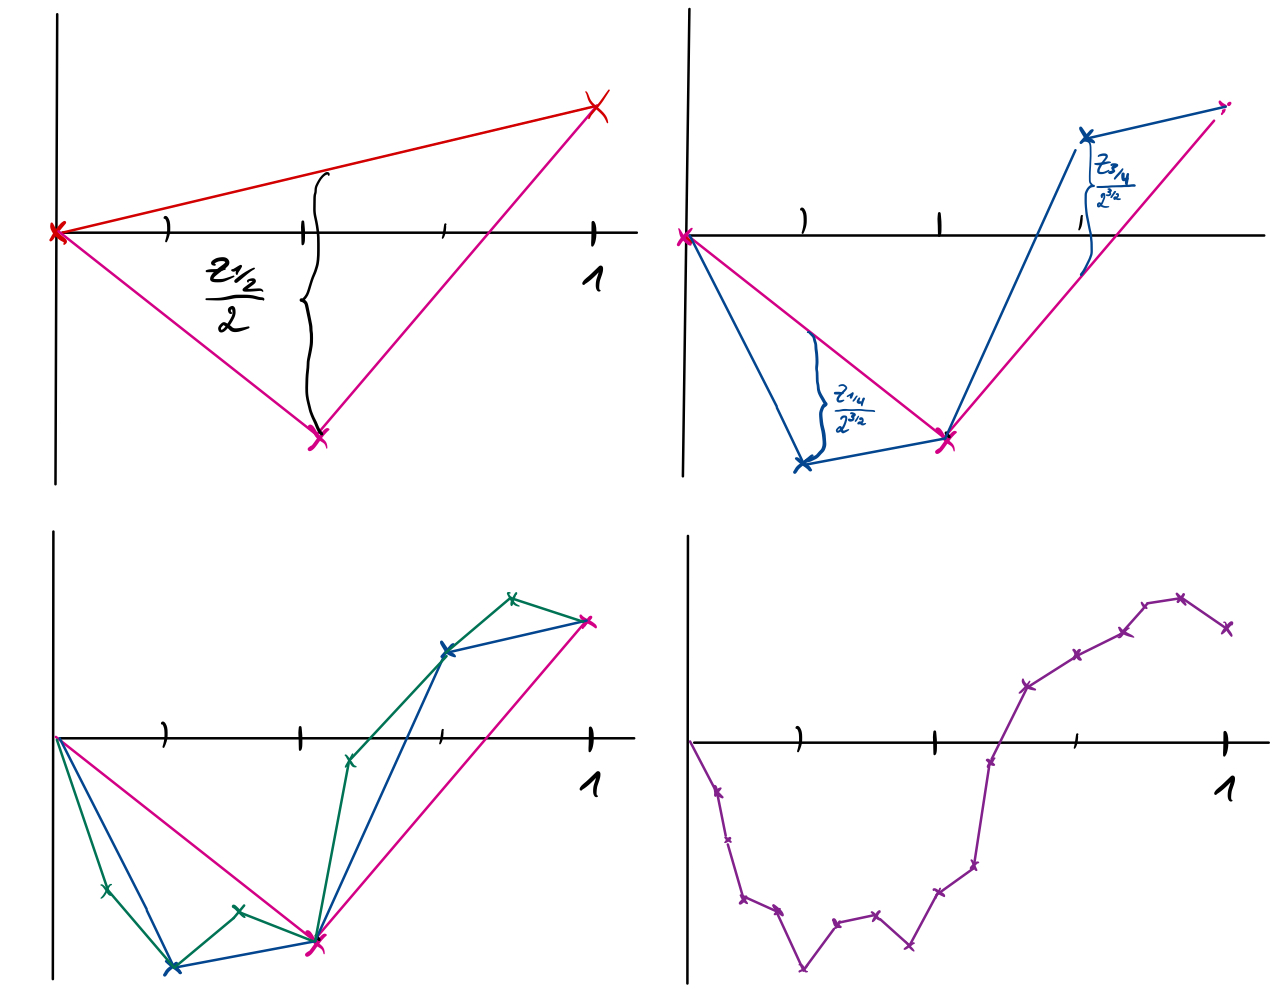
\includegraphics[scale=0.2]{BML2.jpeg}
		\end{center}
		\caption*{First four linearly interpolated discrete Brownian motions from L\'evy's construction}
	\end{figure}

	\begin{lstep}
		The properties (i), (ii), (iv) of a Brownian motion hold on the dyadics.
	\end{lstep}
	One has to check the L\'evy property (stationarity and independence of increments) and the one-dimensional distributions $B_d^{(m)}\sim\mathcal N(0,d)$. The definition of $B^{(m)}_d$ is just made up in a way to produce the right normal distributions for $B^{(m)}_d$. This follows quickly if one knows the following fact on Gaussian vectors. If $X,Y$ are independent $\cN(0,\sigma^2)$, then $X+Y$, $X-Y$ are independent $\cN(0,2\sigma^2)$. The fact follows from writing
	\begin{align*}
		\left(X+Y\atop X-Y\right)= \left(\begin{matrix}
			1 & 1 \\
			1 & -1 
			\end{matrix}\right)\cdot \left(X \atop Y\right)\quad \text{ and }\quad
		\Sigma=
		\left(\begin{matrix}
				1 & 1 \\
				1 & -1 
				\end{matrix}\right)\cdot
		 \left(\begin{matrix}
					1 & 1 \\
					1 & -1 
			\end{matrix}\right)^T =
			\left(\begin{matrix}
				2 & 0 \\
				0 & 2 
		\end{matrix}\right).
	\end{align*}
	Checking independence of increments is a bit similar to the Kolmogorov-Chentsov chaining argument. For neighboring increments the claims follow directly from the construction, an induction is used for the chaining. 
%Pasting together \footnote{Bild}independent copies of $(B_t)_{t\in [0,1]}$  one can check readily that the defining properties hold. As in the proof of Kolmogorov-Chentosv we work with the dyadic numbers $\cD_n = \{ \frac{k}{2^n}\colon k=0,...,2^n\}$ in $[0,1]$. The idea is to define a sequence of "discrete Brownian motions"{} on all $\cD_n$, i.e. stochastic processes that satisfy the right distributional properties (properties (i) and (ii)) on $\cD_n$ and are linearly interpolated in between. The entire sequence is constructed on the same probability space $(\Omega, \mathcal A, \P)$ and converges almost surely uniformly on $[0,1]$. The uniform convergence ensures that the limit has continuous paths (property (iii)), the distributional properties hold on the union $\cD$ of the $\cD_n$, thus, by continuity of sample paths also on $[0,1]$ as the dyadics are dense.
%	\begin{lstep}
%		Construction of the probability space and the discrete Brownian motion on $\cD_n$.
%	\end{lstep}
	%Since $\mathcal D$ is countable there is a probability space $(\Omega, \mathcal A, \P)$ and a sequence of iid $\mathcal N(0,1)$ random variables $(Z_d)_{d\in \mathcal D}$ on $(\Omega, \mathcal A, \P)$. This actually uses the Kolmogorov extension theorem to ensure the existence of the iid sequence (compare Theorem \ref{Folge}). The construction of the discrete Brownian motions on $\cD_n$ is inductively: 
%	\begin{itemize}
%		\item $B_0 = 0$, $B_1 = Z_1$
%		\item Suppose $B_d$ are already defined for all $d\in \cD_{n-1}$. Then define $B_d$, $d\in \cD_n \setminus \cD_{n-1}$ as
%		\begin{align*}
%			B_d = \frac{B_{d-\frac{1}{2^n}} +B_{d+\frac{1}{2^n}}}{2} + \frac{Z_d}{2^{\frac{(n+1)}{2}}}.
%		\end{align*}
%	\end{itemize}
%	The construction is best understood in a picture:\footnote{Bild}

%\begin{lstep}
%	Check the distributional properties (i) and (ii) of a Brownian motion on the dyadics.
%\end{lstep}
%The construction ensures that $(B_d)_{d\in \cD_n}$ and $(Z_d)_{d\in \cD\setminus \cD_n}$ are independent random vectors. This can be used to show that 
%\begin{itemize}
%	\item $B_t - B_s \sim \cN(0,t-s)$ for $s<t$ in $\cD_n$,
%	\item  $B_s - B_r$ independent of $B_t - B_s$ for $r<s<t$ in $\cD_n$.
%\end{itemize}
%The first property follows immediately from the construction, the second is a bit more involved. For the second recall two facts on Gaussian vectors:
%					\begin{itemize}
%						\item $X,Y$ independent $\cN(0,\sigma^2)$ implies that $X+Y$, $X-Y$ are independent $\cN(0,2\sigma^2)$.
%						\item If $(X_1,...,X_n)$ is a Gaussian vector, then the $X_1,...,X_n$ are independent iff $X_1,...,X_n$ is pairwise independent.
%					\end{itemize}
%					The second statement follows directly by checking the covariance matrix $\Sigma$, the first by writing 
%					\begin{align*}
%						\left(X+Y\atop X-Y\right)= \left(\begin{matrix}
%							1 & 1 \\
%							1 & -1 
%							\end{matrix}\right)\cdot \left(X \atop Y\right)
%					\end{align*}
%					and 
%					\begin{align*}
%						\Sigma=
%						\left(\begin{matrix}
%								1 & 1 \\
%								1 & -1 
%								\end{matrix}\right)\cdot
%						 \left(\begin{matrix}
%									1 & 1 \\
%									1 & -1 
%							\end{matrix}\right)^T =
%							\left(\begin{matrix}
%								2 & 0 \\
%								0 & 2 
%						\end{matrix}\right).
%					\end{align*}
%				The distribution of the increments is now computed by induction. A bit similarly to the proof of Kolmogorov-Chentsov we first consider neighboring dyadics. Rewriting the definition of $B_d$ for $d\in \cD_{n+1}$ gives
%				\begin{align*}
%					B_d - B_{d-2^{-n}} &= \frac{B_{d+2^{-n}}-B_{d-2^{-n}}}{2} + \frac{Z_d}{2^{\frac{(n+1)}{2}}}
%				\end{align*}
%				and
%				\begin{align*}
%					B_{d+2^{-n}}- B_d &= \frac{B_{d+2^{-n}}-B_{d-2^{-n}}}{2} - \frac{Z_d}{2^{\frac{(n+1)}{2}}} 
%				\end{align*}
%				The summands on the right hand side are independent and both $\cN(0,2^{-(n+1)})$ by the induction hypothesis. Hence, from the above, the two increments are independent and $\cN(0,2^{-n})$.
%				The same holds for increments of $d\in\cD_{n-1}$ which are not adjacent. (Bild) Left increment only constructed from increments in $(n-1)$st step on the left, right increment from increments in $(n-1)$st step on the right (those are independent by induction hypothesis) plus independent of $Z_d$. $\Rightarrow$ increments are independent. Hence, the (Gaussian) increments are pairwise independent and, thus, independent. But then all increments are also independent.
\begin{lstep}
	The sequence of linearly interpolated discrete Brownian motions almost surely converges uniformly to some limit.
\end{lstep}
Estimating the increments similarly to the proof of Kolmogorov-Chentsov one can use Borel-Cantelli to find a set of probability $1$ on which all increments in $\mathcal D_m$ are small (for $m$ larger than some $m_0(\omega)$). From this one can show that the approximations form Cauchy sequences in $(C([0,1],||\cdot||_\infty)$, thus, converge uniformly to some limits $B(\omega)$.
\begin{lstep}
	The limit is a Brownian motion.
\end{lstep}
It is a crucial advantage of the construction that the continuity of $t\mapsto B_t(\omega)$ follows immediately because uniform limits of continuous functions are continuous. The L\'evy properties can be derived on $\mathcal D$ from the L\'evy properties of the discrete approximations. The construction is such that once a value $B_d$ is defined on a dyadic number it will never be changed again. Hence, for dyadic numbers $B$ satisfies the L\'evy property as the approximations did, the continuity can then be used to transfer the properties to $[0,1]$.
			%Now we need to transfer from $\cD_n$ to $[0,1]$. We now consider the functions obtained from the $B_d$ in $\cD_n$ by linear interpolation. Note: Once a point $t \in \cD_n$ is et it is not changed again.
			%\underline{Claim:} The sequence converges uniformly on $[0,1]$ to a (continuous) function.
			%Why? Let us formalize the functions:
			%\begin{align*}
			%	F_0(t)&\coloneqq \begin{cases}
			%		Z_1 &: t=1 \\
			%		0 &: t=0 \\
			%		\text{linear in between} &\text{ else}
			%	\end{cases} \\
			%	F_n(t) &\coloneqq \begin{cases}
			%		\frac{Z_t}{2^{\frac{(n+1)}{2}}} &: t\in \cD_n \setminus \cD_{n-1} \\
			%		0 &: t \in \cD_{n-1}\\
			%		\text{linear in between} &\text{ else}
			%	\end{cases}
			%\end{align*}
			%Then for all $t\in \cD_n$:
			%\begin{align*}
			%	B_d(t) = \sum_{k=0}^n F_k(t) = \sum_{n=0}^{\infty} F_k(t)
			%\end{align*}
			%We use the series representation to prove the uniform convergence. Recall from Stochastik 1 (exercise) that $\mathbb{P}( \lvert Z_d \rvert \geq c \cdot \sqrt{n}) \leq \exp(-\frac{c^2 n}{2})$ holds for $Z_d \sim \cN(0,1)$.
			%So,
			%\begin{align*}
			%	\sum_{k=0}^{\infty} \mathbb{P}(\exists d\in \cD_k \colon \lvert Z_d \rvert \geq c\sqrt{k}) \overset{\text{subadd.}}&{\leq} \sum_{k=0}^{\infty} \sum_{d \in \cD_k} \mathbb{P}( \lvert Z_d \rvert \geq c \sqrt{k}) \\
			%	&\leq \sum_{k=0}^{\infty} \sum_{d\in \cD_k} e^{-\frac{c^2 k}{2}} \\
			%	&= \sum_{k=0}^n (2^k + 1) e^{-\frac{c^2 k}{2}} \overset{\star}{<} \infty
			%\end{align*}
			%$\star$ if $c > \sqrt{2 \log(2)}$
			%If we fix such a $c$, then Borel-Cantelli implies $ \mathbb{P}(\exists d\in \cD_k \colon \lvert Z_d \rvert \geq c\sqrt{k}\text{ i.o.})=0$. Hence, a.s. there is a random $N = N(\omega )$ such that $\lvert Z_d \rvert < c \sqrt{n}$ for all $d\in \cD_n$ and $n \geq N$. In terms of the (random) functions $F_n$ this means that $\left\Vert F_n \right\Vert_{\infty} \leq c \cdot \sqrt{n} \cdot 2^{-\frac{(n+1)}{2}}$ $\forall n \geq N$. But then
			%\begin{align*}
			%	\left\Vert \sum_{k=0}^{\infty} F_k - \sum_{k=0}^n F_k \right\Vert_{\infty} \overset{\triangle}{\leq} \sum_{k=n+1}^{\infty} \left\Vert F_k \right\Vert_{\infty} \leq \sum_{k=n+1}^{\infty} c \sqrt{n} 2^{-\frac{(k+1)}{2}} \rightarrow 0, \: n \to \infty
			%\end{align*}
		%Hence, $B \coloneqq \sum_{k=0}^{\infty} F_k$ is almost surely the uniform limit of continuous functions and as such also continuous.\\
		%\underline{Claim:} $B$ satisfies the properties of a Brownian motion on $[0,1]$.
		%\begin{enumerate}[label=(\roman*)]
		%	\item \checkmark
		%	\item
		%		Use that centered Gaussian r.v. are independent if all pairwise covariances are zero.\\
		%		Fix $t_1 < ... < t_n$ and sequences $(t_{i,k})_{i,k \in \mathbb{N}} \subseteq \cD$ with $t_{1,k} < ... < t_{n,k}$ and $t_{i,k}\downarrow t_i$. As in (ii), by continuity, vectors $(B_{t_n}-B_{t_{n-1}},...,B_{t_1}-B_0)$ are a.s. limits of $(B_{t_{n,k}}-B_{t_{n-1,k}},...,B_{t_{1,k}}-B_{0,k})$. Hence, they are Gaussian vectors for which we only need covariances. Since the Brownian properties hold on $\cD$ we get 
		%		\begin{align*}
		%			\text{Cov}(B_{t_{i,k}}-B_{t_{i-1,k}},B_{t_{j,k}}-B_{t_{j-1,k}}) &= \mathds 1_{i=j}(t_{i,k}-t_{i-1,k})\\
		%				\overset{k\to\infty}&{=} \mathds 1_{i=j}(t_i-t_{i-1}) \\
		%				&= \text{Cov}(B_{t_i}-B_{t_{i-1}},B_{t_j}-B_{t_{j-1}})
		%		\end{align*}
		%		Hence, the increments are independent and $B_{t+h}-B_t \sim \cN(0,h)$ which is independent of $h$.
		%	\item \checkmark
		%	\item Statement holds for $t_k\in \cD$ which is dense in $[0,1]$. We use a further property of Gaussian vectors: If $(X_n)$ is a sequence of Gaussian vectors for which the expectation vectors and covariance matrices converge and $(X_n)$ converge a.s. to a random vector $X$, then $X$ is Gaussian with the limiting expectation vector and covariance matrix.\\
		%	Take a sequence $(t_n)_{n\in\mathbb{N}}\subseteq \cD$ with $t_n \longrightarrow t$, $n\to\infty$. Since $B$ is continuous, $B_{t_n} \longrightarrow B_t$, $n\to\infty$. Using that $B_{t_n} \sim \cN(0,t_n)$ we obtain $B_t \sim \cN(0,t)$.
		%\end{enumerate}
\end{proof}
Now that the existence is settled we can turn towards properties of the Brownian motion. The aim of the following is to understand the structure of Brownian sample paths, their fluctuations at $0$ and $\infty$, as well as their regularity.
\begin{laussagewerkzeug}
\begin{prop}[Brownian scaling property]
	If $B$ is a Brownian motion and $a>0$, then the process $X_t \coloneqq \frac{1}{a} B_{a^2 t}$, $t\geq 0$, is also a Brownian motion.
\end{prop}
\end{laussagewerkzeug}
The scaling property has an important graphical explanation, zooming out a window of width $a$ and height $\sqrt{a}$ returns (in law) the same graph without the factor $a$.
\begin{figure}[h]
	\begin{center}
		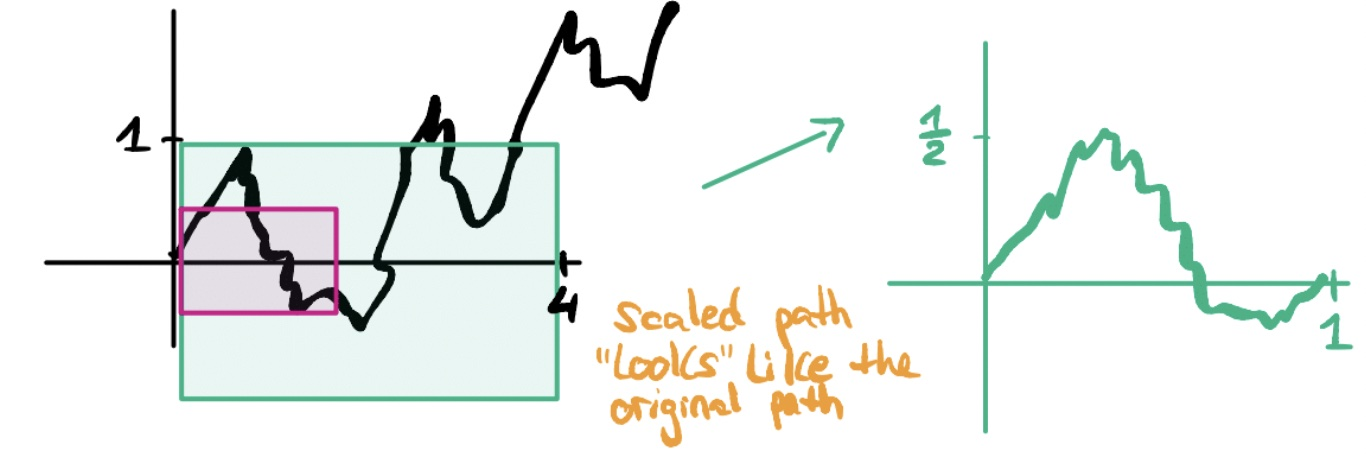
\includegraphics[scale=0.2]{scaling.jpeg}
		\caption*{Scaling property with $a=2$ as zooming in property}
	\end{center}
	\end{figure}
\begin{proof}[Proof]
	We can chose if we check the L\'evy process definition or the Gaussian process definition. Here it is easy to use the Gaussian approach:
	\begin{enumerate}[label=(\roman*)]
		\item \checkmark
		\item Since $$(X_{t_2}- X_{t_{1}},...,X_{t_{k}}-X_{t_{k-1}})=\frac{1}{a}\big( B_{a^2 t_2}-B_{a^2 t_{1}},...,B_{a^2 t_k}- B_{a^2 t_{k-1}}\big)$$ the independence of increments is inherited from $B$, just as the independence of $h$ in $X_{t+h}-X_t = \frac{1}{a}(B_{a^2t+a^2 h}-B_{a^2 t})$ is inherited from $B$.
		\item \checkmark
		\item $X_t = \frac{1}{a} B_{a^2 t} \sim \cN(0,t)$ follows from the scaling property of $\cN(\mu,\sigma^2)$
	\end{enumerate}
\end{proof}
In order to get an idea why the scaling property is useful let us consider first hitting times. The scaling property tell us that enlarging (resp. shrinking) space by a constant has the same effect than speeding up/slowing down time with the square-root of the constant. Morally, the time to a point which is $b$-times further away should thus be $b^2$-times longer. Here is an example computation for 
\begin{align*}
	T(a,b)=\inf \{ t\colon B_t = a \text{ or }B_t = b\},\quad a<0<b.
\end{align*}	
Using the scaling property gives
\begin{align*}
	 T(a,b)  \overset{\text{(d)}}&{=} \inf \Big\{ t\colon b B_{\frac{1}{b^2}t} = a \text{ or } b B_{\frac{1}{b^2}t}=b \Big\} 
	= b^2   \inf\Big\{ t \colon B_t = \frac{a}{b} \text{ or } B_t = 1\Big\} 
	= b^2  T\Big(\frac{a}{b},1\Big).
\end{align*}
In particular, chosing $a=-b$ we have the identity $\E\big[ T(-b,b)\big] = b^2 \E \big[ T(-1,1)\big]$. This is a very typical application of the scaling property, in order to compute the expectation of all hitting times it is only needed to compute $\E\big[ T(-1,1)\big]$.\smallskip

Extremely useful tools to work with the Brownian motion are the Markov  and martingale property for which we use the natural filtration $\cF_s \coloneqq \sigma(B_t : t\leq s)$. Here are the two properties:
\begin{laussagewerkzeug}
\begin{prop}
	Let $(B_t)_{t\geq 0}$ be a Brownian motion on $(\Omega, \mathcal A, \P)$.
	\begin{enumerate}[label=(\roman*)]
		\item
			$B$ has the simple Markov property, that is,
			$$B_t^{(s)} \coloneqq B_{t+s} - B_s, \quad t\geq 0,$$ is a Brownian motion independent of $\cF_s$ for all $s\geq 0$.
		\item
			$B$ is a continuous-time $(\mathcal F_s)$-martingale, that is,
			$$\E[\lvert B_t \rvert ]<\infty\quad \text{and}\quad \E [B_t|\cF_s] = B_s\,\text{ a.s. for all }t\geq s.$$
	\end{enumerate}
\end{prop} 
\end{laussagewerkzeug}
\begin{figure}[h]
	\begin{center}
		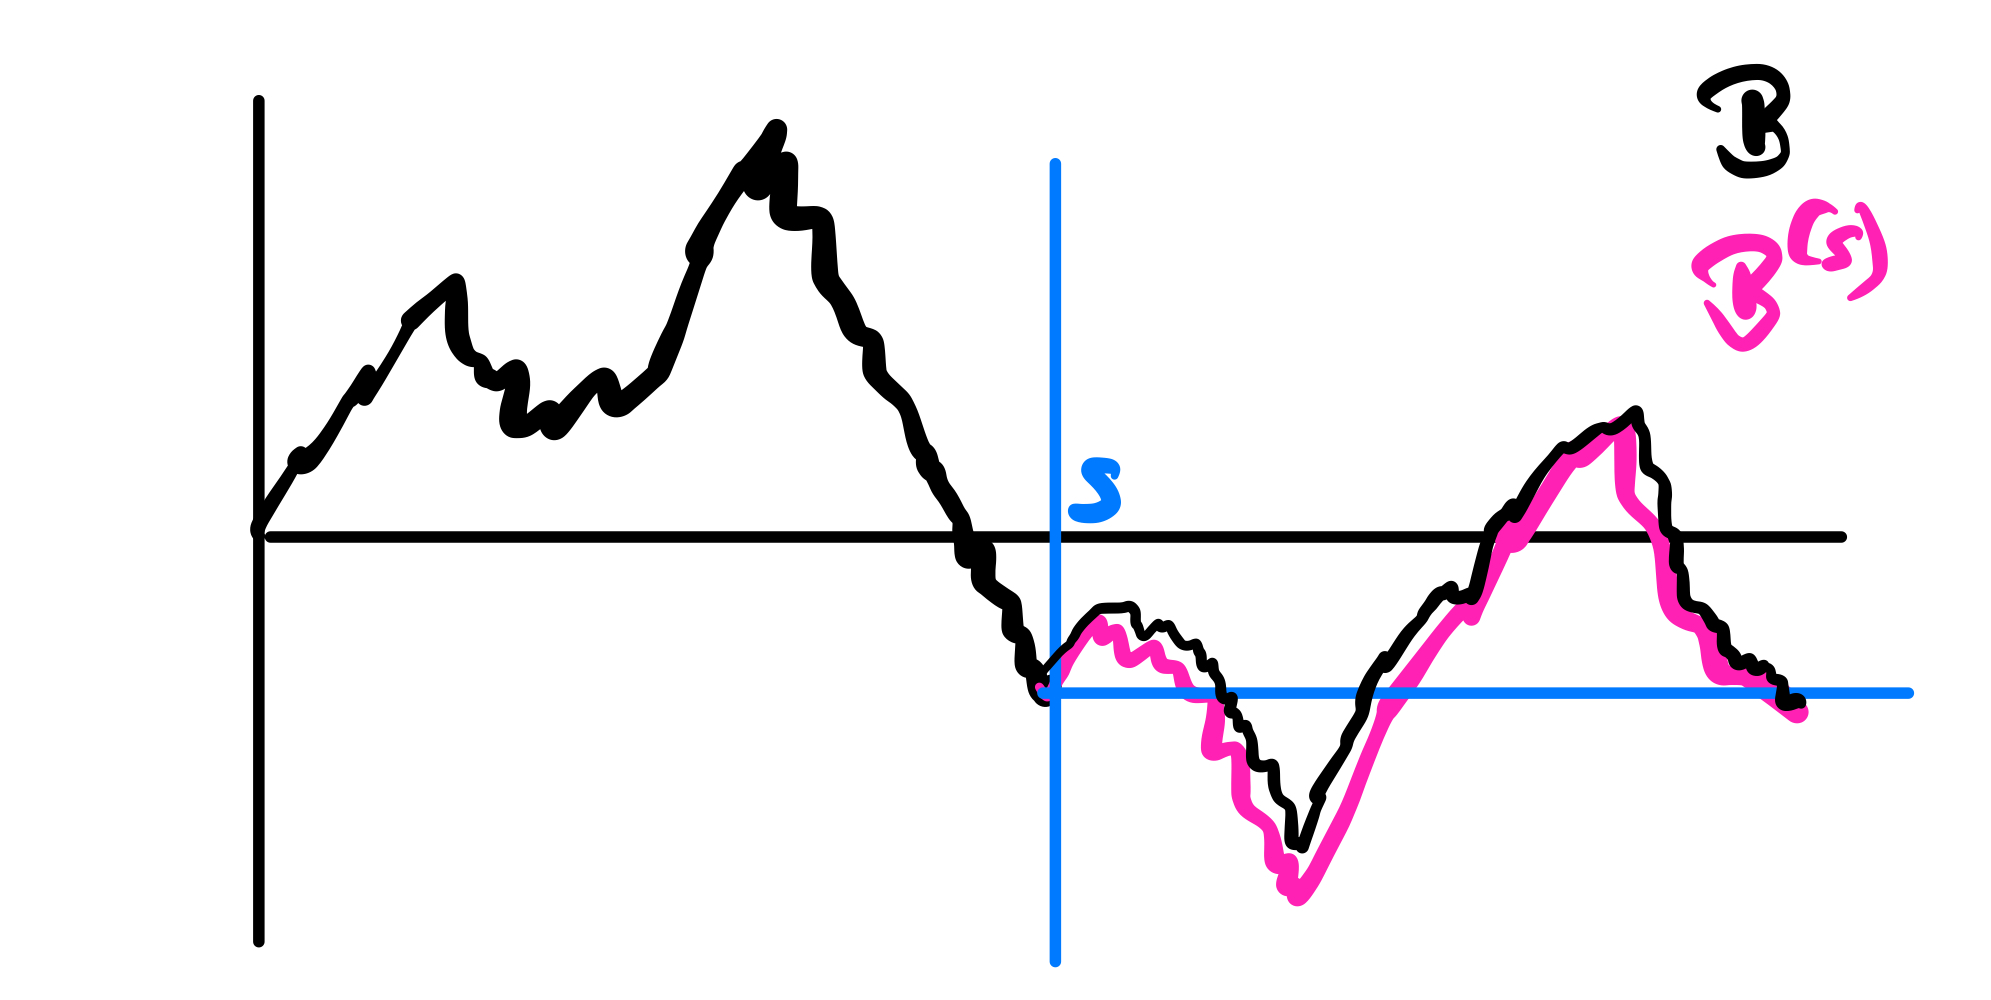
\includegraphics[scale=0.1]{markov.jpeg}
		\caption*{Graphical visualisation of the simple Markov property}
	\end{center}
	\end{figure}

To clarify the first statement let us recall the definition of independence. The statement is to be read as independence of $\mathcal F_s=\sigma(B_t: t\leq s)$ from $\sigma(B_t^{(s)}: t\geq 0)$ because independence of random variables is always defined through the generated $\sigma$-algebras. In fact, this is much more than what is called the Markov property in continuous time which only requires the independence of $B^{(s)}$ from $\mathcal F_s$ but not that $B^{(s)}$ has the same distribution as $B^{(0)}$. 
\begin{proof}[Proof]
(i) Independence of $\sigma$-algebras only needs to be checked on $\cap$-stable generators, Proposition \ref{unabh}. Hence, it suffices to 
check that $B_{r_1},...,B_{r_n}$ and $B_{t_1}^{(s)},...,B_{t_r}^{(s)}$ are independent for all choices of $r_1\leq ....\leq r_n\leq s$ and $0\leq t_1\leq ...\leq t_r$. 
			Since the Brownian motion $(B_t)_{t\geq 0}$ is a Gaussian process the vector 
			$(B_{r_1},...,B_{r_n},B_s,B_{s+t_1},...,B_{s+t_r})$ is Gaussian. Multiplying the vector with a cleverly chosen matrix (which?) gives $(B_{r_1},..., B_{r_n},B_{s+t_1}-B_s,..., B_{s+t_r}-B_{s})$ which then is also a Gaussian vector. To prove independence of the first $n$ from the last $r$ entries it is thus enough to prove that all covariances $\Cov(B_r,B_{s+t}-B_s)$ vanish for $r\leq s\leq s+t$ as independence and uncorrelated is equivalent for entries of Gaussian vectores. But this is simple:
			\begin{align*}
				\text{Cov}(B_{r},B_{s+t}-B_s) &= \E \big[ B_{r}(B_{s+t}-B_s)\big] \\
												&= \E \big[B_{r}B_{s+t}\big] - \E \big[B_{r}B_s\big]\\
												&=\text{Cov}(B_{r},B_{s+t})+\text{Cov}(B_{r},B_s)\\
												&= r - r = 0
			\end{align*}
			
	(ii) The integrability is easy, all $B_t$ are Gaussian. For the martingale property we use a trick: Use $B_t = (B_t-B_s)+B_s$ and the statements from (i) to get almost surely
			\begin{align*}
				\E [B_t \,|\,\cF_s] = \E [B_t - B_s\,|\,\cF_s] + \E[B_s\,|\,\cF_s] 
										= \E [B_t^{(s)}\,|\,\cF_s] + B_s 
										\overset{\text{(i)}}{=} \underbrace{\E[B_t^{(s)}]}_{=0} + B_s=B_s.
			\end{align*}
\end{proof}
\marginpar{\textcolor{red}{Lecture 24}}

Here is a nice application of the martingale property:
\begin{laussagewerkzeug}
\begin{prop}[Brownian law of large numbers]
	If $(B_t)_{t\geq 0}$ is a Brownian motion, then $\lim\limits_{t\to\infty} \frac{1}{t}B_t = 0$ almost surely.
\end{prop}
\end{laussagewerkzeug}
\begin{proof}[Proof]
	It follows from the definition that the increments
	$(B_n-B_{n-1})_{n\in\mathbb{N}}$ are iid $\cN(0,1)$ because independence of infinitely many events or random variables is only defined through all finite subsets of the index set (Definition \ref{def:unab}). Hence, the strong law of large numbers yields
	\begin{align*}
		\lim_{n\to\infty} \frac{1}{n} B_n = \lim_{n\to\infty} \frac{1}{n}\sum_{k=1}^n (B_{k}-B_{k-1})  \overset{\text{LLN}}{=} \E[B_1-B_0] = 0
	\end{align*}
	almost surely. Thus the statement of the theorem is simple on $\mathbb{N}$ and it suffices to control $B$ between the integers. For that purpose define $$Y_n \coloneqq \sup_{t\in[n,n+1]} \lvert B_t - B_n \rvert = \sup_{t\in[n,n+1]\cap \mathbb{Q}} \lvert B_t - B_n \rvert.$$ The second equality follows from the continuity of sample paths (which we can assume to be continuous for all $\omega\in \Omega$).
	Then $Y_0,Y_1,...$ is an iid sequence because $B_t- B_n$ and $B_s - B_m$ are independent increments. If we can prove that $\E [\lvert Y_0 \rvert]< \infty$ then, again by the strong law of large numbers, $$\lim\limits_{n\to\infty} \frac{1}{n}\sum\limits_{k=0}^n Y_k = \E[Y_0] < \infty$$ almost surely which in particular implies $\frac{1}{n}Y_n \rightarrow 0$, $n\to\infty$, almost surely. Combined with the law of large number on the integers it follows ($Y_n$ is the largest absolute deviation from $B_n$ in $[n,n+1]$, draw a picture!) that
	\begin{align*}
		0=\liminf_{t\to\infty}\frac{B_{\lfloor t \rfloor}-Y_{\lfloor t \rfloor}}{t}\leq\liminf_{t\to\infty}\frac{1}{t}B_t\leq \limsup_{t\to\infty}\frac{1}{t}B_t &\leq \limsup_{t\to\infty}\frac{B_{\lfloor t \rfloor}+Y_{\lfloor t \rfloor}}{t} = 0
	\end{align*}
	almost surely and the proof of the theorem is complete. However, we need to verify that $\E[\lvert Y_0 \rvert ]< \infty$ which, surprisingly, follows from martingale theory. Define
	\begin{align*}
		M_n^{(m)} \coloneqq B_{n\cdot 2^{-m}}, \quad n=0,...,2^m,
	\end{align*}
	which is a discrete-time $(\mathcal F^{(m)}_n)_{n=0,...,2^m}:=(\mathcal F_{n 2^{-m}})_{n=0,...,2^m}$ martingale. In fact, $M^{(m)}$ equals the Brownian motion at discrete times so that the martingale property follows by restricing process and filtration to the same increasing subset of time. The Doob inequality with $p=2$ then implies
	\begin{align*}
		\E\Big[ \big(\max_{n\leq 2^m} M_n^{(m)}\big)^2\Big] \overset{\text{Doop with }p=2}{\leq} 4 \cdot \E\big[ (M_{2^m}^{(m)})^2\big] = 4 \cdot \E \big[ B_1^2\big] = 4,
	\end{align*}
	for all $m\in \N$. Hence, the sequence $\big(\max_{n\leq 2^m} M_n^{(m)}\big)_{m\in\mathbb{N}}$ is bounded in $L^2$, in particular uniformly integrable. Surprisingly, we can now finish the proof with a new kind of trick. Continuity of Brownian motion implies that $$Y_0 = \sup_{t\in[0,1]\cap \Q}\lvert B_t \rvert  = \lim_{m\to\infty} \max_{n\leq 2^m} M_n^{(m)}$$ holds almost surely. But this means that $Y_0$ is an almost sure limit of a uniformly integrable sequence. By Theorem \ref{generalized_DCT} the convergence also holds in $L^1$ and this implies that $Y_0\in L^1$.
\end{proof}
The law of large number is a very rough statement about the fluctuations of $B$ at infinity. It can be interpreted such that a Brownian motion eventually stays in every linear cone. We will see below that a Brownian motion does not stay within any "{}square-root domain", see the drawing. In fact, a much better statement holds, a Brownian motion oscillates precisely of the order $\sqrt{2t \log (\log (t))}$, this is the so-called law of the iterated logarithm: $$\limsup_{t\to\infty}\frac{|B_t|}{\sqrt{2t \log( \log(t))}}=1.$$ The limit superior is needed here as the Brownian motion oscillates between $\sqrt{2t \log( \log(t))}$ and $-\sqrt{2t \log( \log(t))}$, the limit does not exist.
\begin{figure}[h]
	\begin{center}
		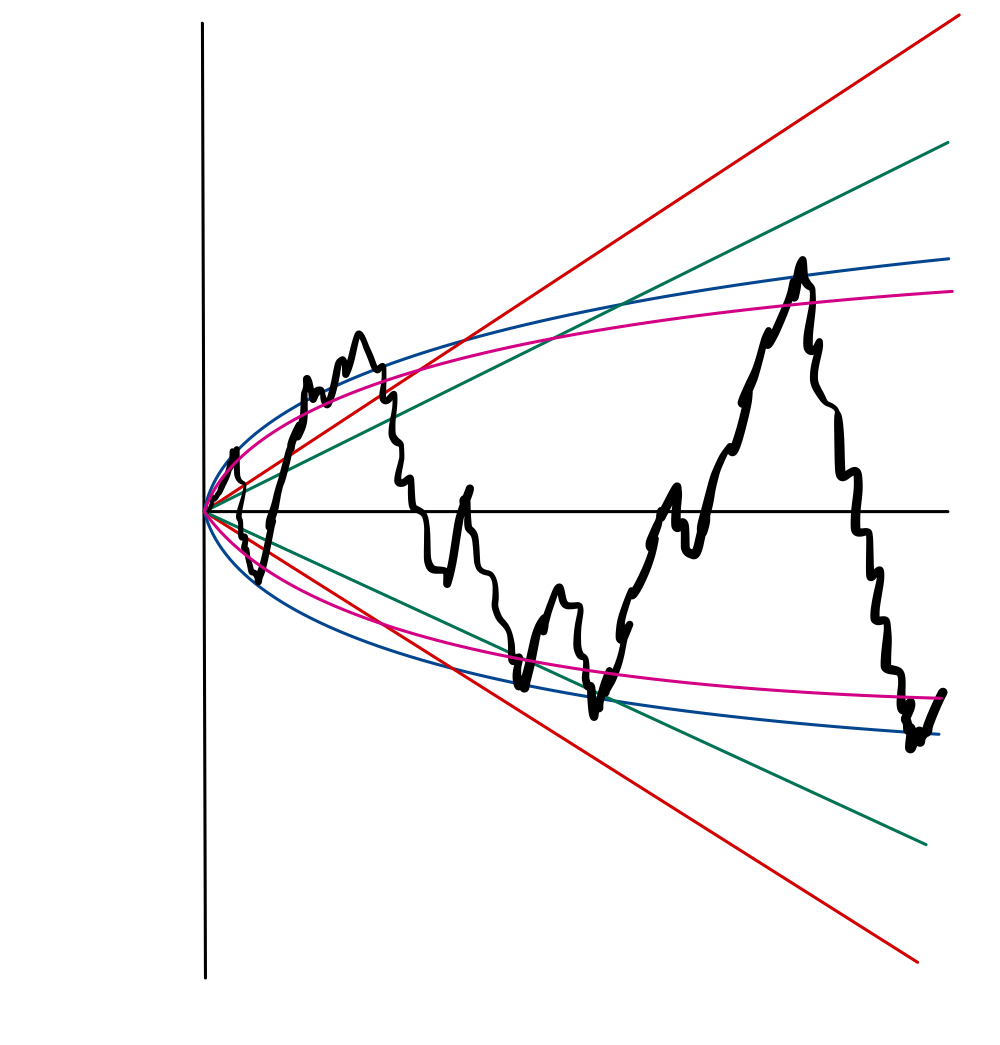
\includegraphics[scale=0.1]{cones.jpeg}
		\caption*{Linear, $\sqrt{2t \log(\log(t))}$ in blue, and $\sqrt{t}$ in purple}
	\end{center}
\end{figure}

 In particular, this shows that $\lim_{t\to\infty}|B_t|=\infty$ almost surely which does not follow from the law of large numbers alone ($B$ could also be bounded or converge). The unboundedness statement is simple and can be proved in many elementary ways, for instance using Borel-Cantelli or the Optional Stopping Theorem for the discrete martingale $(B_n))_{n\in\N}$, give it a try!
\begin{luebung}
	 Show that almost surely the Brownian motion is unbounded.
 \end{luebung}
Many statements at infinity can be translated into statements at zero using the following time-inversion property.
\begin{laussagewerkzeug}
\begin{prop}[Brownian time-inversion]
	If $(B_t)_{t\geq 0}$ is a Brownian motion, then also 
	\begin{align*}
		X_t\coloneqq \begin{cases}
					t\, B_{\frac{1}{t}} &: t> 0 \\
					0 &: t=0
					\end{cases}
	\end{align*}
	is a Brownian motion.
\end{prop}
\end{laussagewerkzeug}
\begin{proof}[Proof] 
	We use the characterisation of a Brownian motion as a Gaussian process and check that $X$ is a Gaussian process with the appropriate covariance function and continuous sample paths.\smallskip

	(i) $X$ is clearly a Gaussian process since the finite-dimensional marginals are $(X_{t_1},...,X_{t_k})=(t_1 B_{t_1^{-1}},...,t_k B_{t_k^{-1}})$ which can be rewritten as a diagonal matrix multiplied to the Gaussian vector $(B_{t_1^{-1}},...,B_{t_k^{-1}})$ and, hence, is a Gaussian vector itself.\smallskip

	(ii) The covariance function can be computed as follows:
	$$\text{Cov}(X_s,X_t) = s\cdot t \cdot \text{Cov}(B_{\frac{1}{s}},B_{\frac{1}{t}}) = s\cdot t \cdot \frac{1}{s}\wedge \frac{1}{t}=s\wedge t,$$ which is the Brownian covariance function.\smallskip

	(iii) $X$ is continuous for $t>0$ as a concatenation of continuous functions. The almost sure continuity at $0$ follows from the Brownian law of large numbers: $$\lim_{t\to 0} X_t = \lim_{t\to 0} t B_{\frac{1}{t}} = \lim_{t\to\infty} \frac{1}{t} B_t \overset{\text{LLN}}{=} 0 = X_0.$$ Hence, $X$ is almost surely continuous on $[0,\infty)$.
	\end{proof}
The next property is a very important property to study the structure of sample paths. We prove that the infinitesimal behavior at zero (using the simple Markov property also at all other fixed times $t$ and using time-inversion also at infinity) satisfies a zero-one law. The same statement holds much more generally for all reasonable Markov processes in continuous time.
\begin{laussagewerkzeug}
\begin{theorem}[Blumenthal zero-one law]
	Define $\cF_{0+} =\bigcap_{s>0}\cF_s$, then $\cF_{0+}$ is trivial, i.e. $\mathbb{P}(A)\in\{0,1\}$ for all $A\in \cF_{0+}$.
\end{theorem}
\end{laussagewerkzeug}
\begin{proof}[Proof]
	The proof consists of two major steps which combined result in the self-independence of $\cF_{0+}$ from which the claim follows.
	\begin{lstep}
		$\cF_{0+}$ is independent of $\sigma(B_t:t>0)$.
	\end{lstep}
	To prove the claim we first fix $A\in \cF_{0+}$, $0 < t_1 < ... <t_k$, and $f\colon \mathbb{R}^k \to \mathbb{R}$ bounded continuous and prove that
	\begin{align}\label{equ:ind}
		\E \left[ \mathbf 1_A f(B_{t_1},...,B_{t_k}) \right]=\mathbb{P}(A) \E \left[ f(B_{t_1},...,B_{t_k})\right].
	\end{align}
	Since $f$ and Brownian sample paths are continuous, the dominated convergence theorem yields
	\begin{align*}
		\E \left[ \mathbf 1_A f(B_{t_1},...,B_{t_k}) \right] \overset{\text{DCT}}{=} \lim_{\varepsilon \to 0} \E \left[ \mathbf 1_A \cdot f(B_{t_1}-B_{\varepsilon},...,B_{t_k}-B_{\varepsilon})\right].
	\end{align*}
	If $t_1>\varepsilon$, then, by the simple Markov property, the random variables $B_{t_1}-B_{\varepsilon},...,B_{t_k}-B_{\varepsilon}$ are independent of $\cF_{\varepsilon}$ and thus independent of its sub-$\sigma$-algebra $\cF_{0+}$ (the independence property needs to hold only for less events). Factorising the expectation and using dominated convergence backwards leads to
	\begin{align*}
		\E \left[ \mathbf 1_A f(B_{t_1},...,B_{t_k}) \right]=  \E \left[ \mathbf 1_A \right] \cdot \E\left[f(B_{t_1},...,B_{t_k})\right]
	\end{align*}
	which proves \eqref{equ:ind}. To deduce the claimed independence of the $\sigma$-algebras recall from Proposition \ref{unabh} that independence only needs to be checked on $\cap$-stable generators. A $\cap$-stable generator of $\sigma(B_t:t>0)$ is the set of events $\{(B_{t_1},..., B_{t_k})\in C\}$ for arbitrary $0 < t_1 < ... <t_k$ and Borel-sets $C\in \mathcal B(\R^k)$. The preimages for single times are not $\cap$-stable. Approximating the discontinuous indicator functions $\mathbf 1_{C}$ by the bounded continuous functions $f^{\varepsilon}_C$ from the proof of Proposition \ref{theorem_4124} we obtain from the above, once again referring to dominated convergence, 
	\begin{align*}
		\P(A\cap \{(B_{t_1},...,B_{t_k})\in C\})
		&=\E[ \mathbf 1_A\cdot \mathbf 1_{C}(B_{t_1},...,B_{t_k})]\\
		&=\lim_{\varepsilon \to 0}\E \left[ \mathbf 1_A \cdot f_C^\varepsilon (B_{t_1},...,B_{t_k})\right]\\
		&= \E[\mathbf 1_A] \E \left[ \mathbf 1_C(B_{t_1},...,B_{t_k})\right]\\
		&= \P(A) \cdot \P ((B_{t_1},...,B_{t_k})\in C).
	\end{align*}
	%
	%
	%Hence, for all $A\in \cF_{0+}$,
	%\begin{align}\label{ind}
	%	\E \left[ \mathds 1_A g(B_{t_1},...,B_{t_k})\right] &= \lim_{\varepsilon \to 0} \mathbb{P}(A) \E \left[ g(B_{t_1}-B_{\varepsilon},...,B_{t_k}-B_{\varepsilon})\right]
	%		= \mathbb{P}(A) \E \left[ g(B_{t_1},...,B_{t_k})\right].
	%\end{align}	
	\begin{lstep}
		$\sigma(B_t \colon t > 0)=\sigma(B_t \colon t\geq 0)$
	\end{lstep}
	The reason is simple: the additional random variable $B_0$ is $\sigma(B_t \colon t > 0)$-measurable since the continuity of sample paths yields $B_0 = \lim_{n\to\infty} B_{\frac{1}{n}}$ and measurability of sequences of random variables transfers to the limit (compare Proposition \ref{prop:limits}).\smallskip

	The claim of the proposition can now be proved easily. Since $\cF_{0+}\subseteq \sigma(B_t \colon t\geq 0)$ the first two steps combined show that $\cF_{0+}$ is independent of itself. But this implies $\mathbb{P}(A)= \mathbb{P}(A\cap A) = \mathbb{P}(A)\cdot \mathbb{P}(A)$ for all $A\in \cF_{0+}$, hence, $\mathbb{P}(A)\in \{0,1\}$.
\end{proof}
As an application we deduce the first property on the fluctuations of paths. 
\begin{laussagewerkzeug}
\begin{corollary}\label{kor_sup}
	If $B$ is a Brownian motion on $(\Omega, \mathcal A, \P)$, then
	%If $\varepsion>0$ 
	%We have $\forall \varepsilon >0$, almost surely,
	\begin{align*}
		\sup_{t\in [0,\varepsilon]} B_t > 0\quad \text{ \underline{and} }\quad  \inf_{t \in [0,\varepsilon]} B_t < 0,\quad \forall \varepsilon>0,
	\end{align*}
	hold almost surely.
\end{corollary}
\end{laussagewerkzeug}
\begin{proof}[Proof]
	Take an arbitary sequence $\varepsilon_n \downarrow 0$ and consider 
	\begin{align*}
		A \coloneqq \bigcap_{n\in\mathbb{N}} \Big\{ \omega\in\Omega \colon \sup_{0\leq s \leq \varepsilon_n} B_s(\omega) > 0\Big\}\in \mathcal F_{0+}
	\end{align*}
	Note that all appearing sets are measurable since $\sup_{s \leq \varepsilon_n}B_s=\sup_{s \leq \varepsilon_n, s\in \Q}B_s \in \mathcal F_{\varepsilon_n}$ (countable supremum over $\mathcal F_{\varepsilon_n}$-measurable mappings). If we can show that $\P(A)=1$, then the claim is proved for the supremum.	Since the events of the intersection are decreasing and $\varepsilon_n\to 0$ it follows that $A\in \mathcal F_s$ for all $s>0$, hence, $A\in \mathcal F_{0+}$. Now the Blumenthal zero-one law implies $\mathbb{P}(A)\in \{0,1\}$. Using monotonicity of measures gives
	\begin{align*}
		\mathbb{P}(A) = \lim_{n\to\infty} \mathbb{P}\big(\sup_{s\leq \varepsilon_n}B_s > 0\big) \geq \lim_{n\to\infty} \mathbb{P}(B_{\varepsilon_n}>0) = \frac{1}{2}
	\end{align*}
	because $B_{\varepsilon_n}\sim \cN(0,\varepsilon_n)$. Hence, $\mathbb{P}(A)=1$ must hold. To prove the claim on the infimum quickly check the following exercise: 
	\begin{luebung}
		If $B$ is a Brownian motion, then $-B$ is also a Brownian motion.
	\end{luebung}	
	The claim for the supremum applied to the Brownian motion $-B$ gives the claim for the infimum. 
\end{proof}
As a direct consequence a simple roughness property can be proved. No matter how small an interval $[a,b]$ a Brownian path $t\mapsto B_t$ is not increasing or decreasing on $[a,b]$!
\begin{lSatzHerz}
\begin{theorem}
	Brownian sample paths are almost surely not monotone on any interval.
\end{theorem}
\end{lSatzHerz}
\begin{figure}[h]
	\begin{center}
		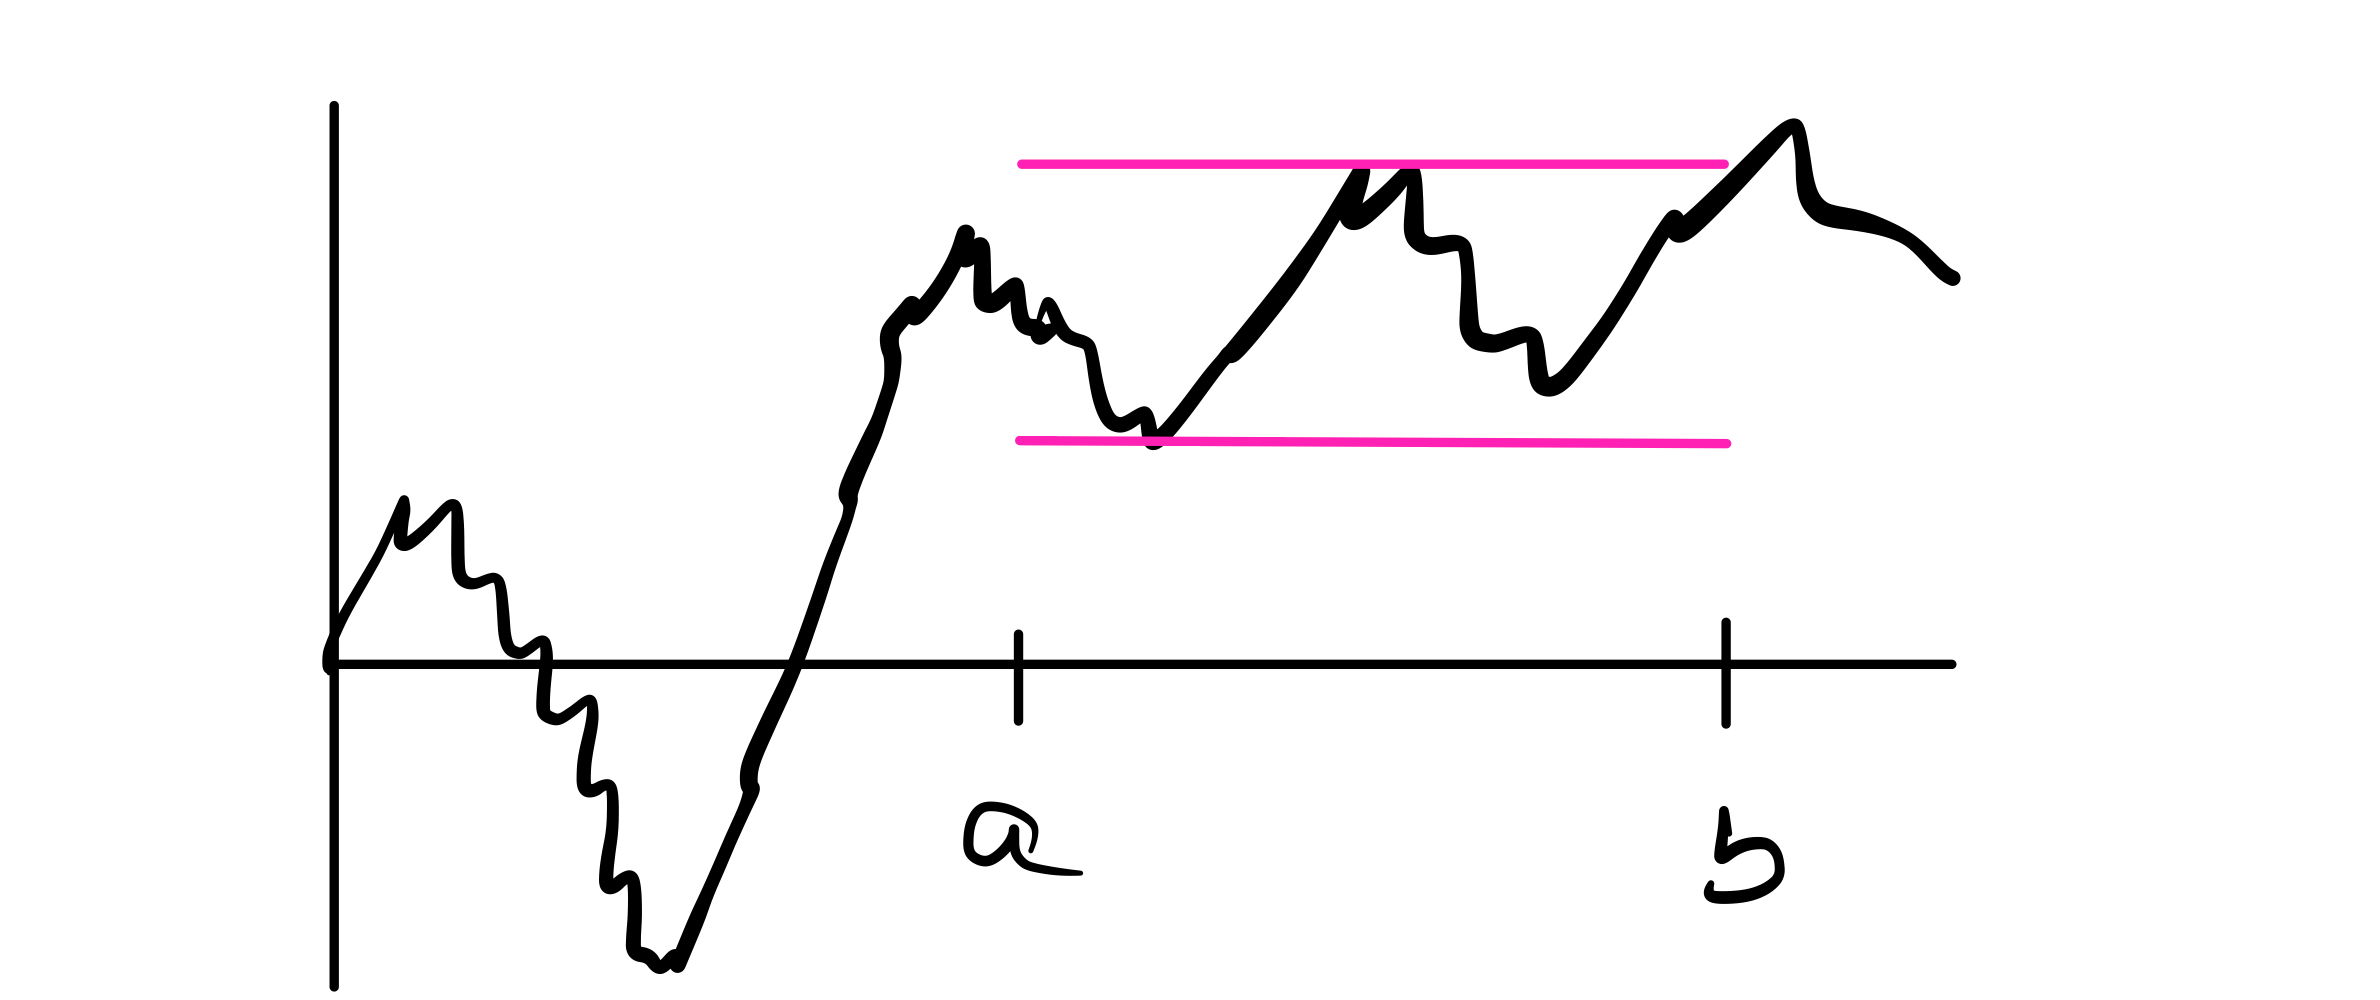
\includegraphics[scale=0.1]{monotonepaths.jpeg}
		\caption*{Brownian motion is nowhere monotone}
	\end{center}
	\end{figure}
\begin{proof}[Proof]
	The claim is a direct consequence of Corollary \ref{kor_sup} and the simple Markov property. By the simple Markov property we find almost surely that for all $q\in \mathbb{Q_+}$
	\begin{align*}
		0 < \sup_{t\leq \varepsilon} B_t^{(q)} \overset{\text{Def}}{=} \sup_{t\leq \varepsilon} \left(B_{q+t} - B_q \right) = \sup_{t\leq \varepsilon}B_{q+t} - B_q
	\end{align*}
	and 
	\begin{align*}
		0 > \inf_{t\leq \varepsilon} B_t^{(q)} \overset{\text{Def}}{=} \inf_{t\leq \varepsilon} \left(B_{q+t} - B_q \right) = \inf_{t\leq \varepsilon}B_{q+t} - B_q
	\end{align*}
	Hence, almost surely it holds that $B_q < \sup_{t\leq \varepsilon} B_{q+t}$ and $ \inf_{t\leq \varepsilon} B_{q+t}< B_q$. Since every interval contains a rational number the claim follows.
\end{proof}
After these first rather simple roughness results of qualitative nature we now come to the first deep result on the path-regularity of the Brownian motion.
\begin{lSatzHerz}
\begin{theorem}
	The sample paths of a Brownian motion on $(\Omega, \mathcal A, \P)$ are almost surely \underline{not} locally H\"older continuous of index $\frac{1}{2}$ but they are locally H\"older continuous of index $\gamma$ for all $\gamma<\frac{1}{2}$.
\end{theorem}
\end{lSatzHerz}
\begin{proof}[Proof]
	Before going into the proof let us quickly discuss the statement. If $B=(B_t)_{t\geq 0}$ is defined on $(\Omega, \mathcal A, \P)$ then it is not clear if the subset $$C:=\Big\{\omega\in \Omega\,\Big|\, t\mapsto B_t(\omega)\text{ is locally H\"older continuous of index }\frac{1}{2}\Big\}$$ of $\Omega$ is measurable in $\mathcal A$ as $C$ cannot be written in terms of countably many $B_t$. Hence, the statements $\P(C)=1$ or $\P(C^c)=0$ are problematic and possibly not defined. We will construct a very explicit measurable subset of $C$ with measure $1$.
	\begin{lstep}
		Brownian sample paths are almost surely \underline{not} H\"older continuous of index $\frac{1}{2}$ at $0$.
	\end{lstep}
	We are going to show that, for all $k>0$,
	\begin{align*}
		\mathbb{P}\left(\inf\{ t>0\colon |B_t| \geq k \cdot \sqrt{t}\}=0\right)=1,%\quad\text{ and }\quad
		%\mathbb{P}\left(\inf\{ t>0\colon B_t \leq -k \cdot \sqrt{t}\}=0\right)=1
	\end{align*}
	which means that the Brownian motion never stays within square-root domains at zero (see the drawing).
	\begin{figure}[h]
		\begin{center}
			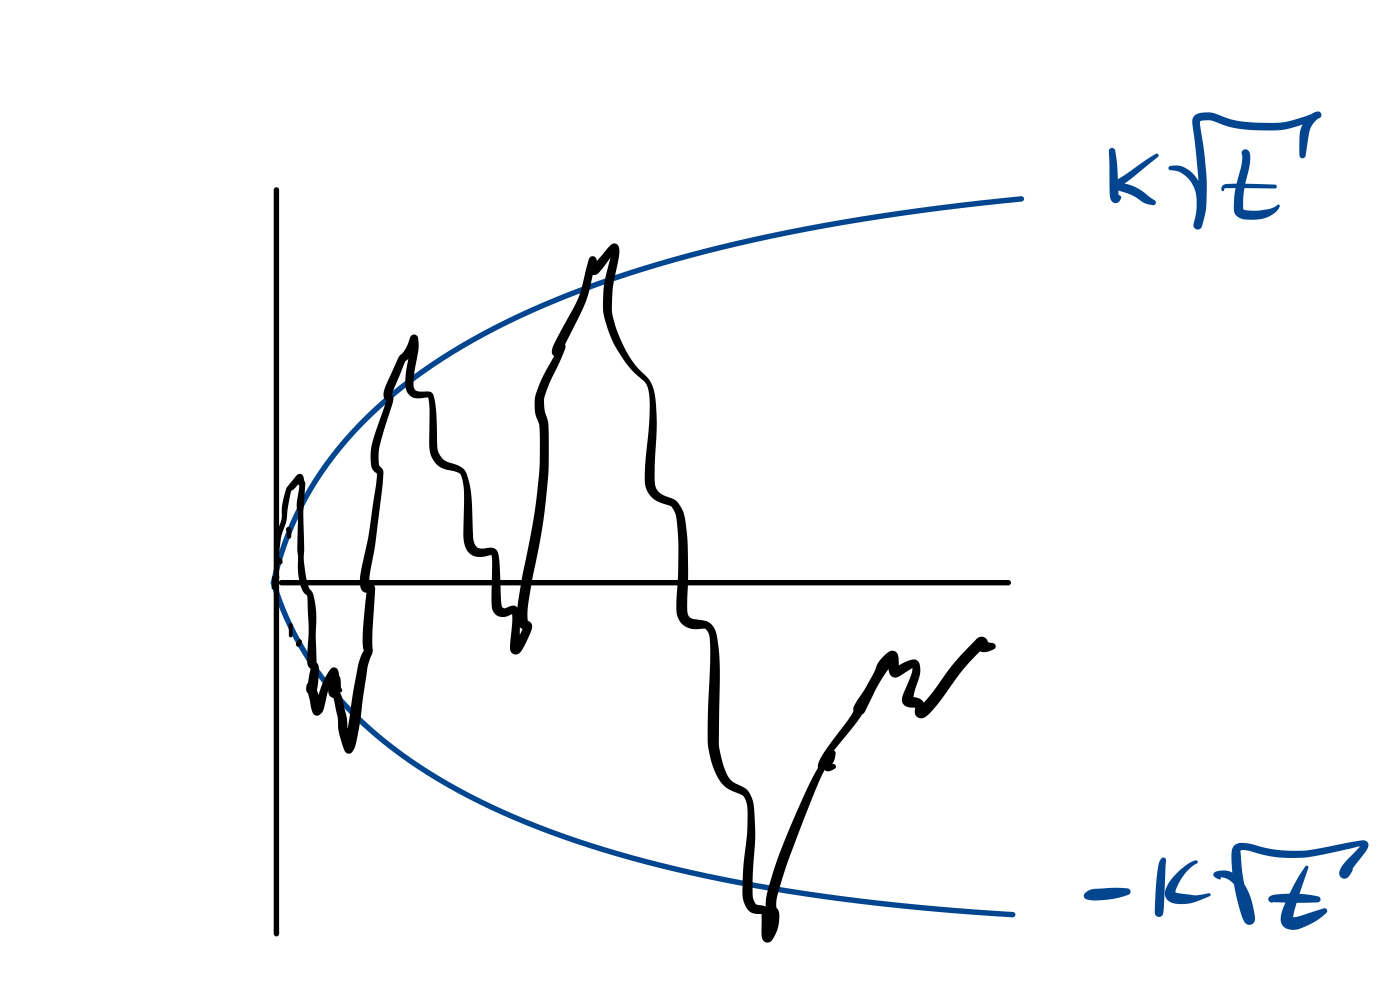
\includegraphics[scale=0.12]{sqrt.jpeg}
		\end{center}
	\end{figure}	
	The probabilities can be computed using the Blumenthal zero-one in very much the same way as we did in the proof of Corollary \ref{kor_sup} for the constant $0$ function instead of the square-root function (supremum up to time $t$ positive is equivalent to the first hitting of $[0,\infty)$ smaller than $t$). Defining $$A^{(k)} =\big\{\omega\in \Omega\,|\, \inf\{t>0\colon |B_t(\omega)| \geq k\cdot\sqrt{t}\}=0\big\}$$ and 	
	$$A^{(k)}_s = \big\{\omega\in \Omega\,|\, \inf\{t>0\colon |B_t(\omega)| \geq k\cdot\sqrt{t}\}\leq s\big\}\in \cF_s,$$ we have $A^{(k)} = \bigcap_{s>0} A^{(k)}_s \in \cF_{0+}$. Since without loss of generality we assumed that all sample paths are continuous (e.g. canonical construction using the Wiener measure)	all these sets are measurable as the infimum only needs to be taken over rational time points. Hence, $\mathbb{P}(A^{(k)}) = 0$ or $\mathbb{P}(A^{(k)})=1$ by the Blumenthal zero-one law. Monotonicity of measures and the scaling property of Gaussian random variables gives
	\begin{align*}
		\mathbb{P}\big(A^{(k)}\big) &=\lim_{s\to 0} \mathbb{P}\big(A^{(k)}_s\big) \\
					&= \lim_{s\to 0} \mathbb{P}\Big(\inf\Big\{t>0\colon \frac{1}{\sqrt{t}}|B_t| \geq k\Big\}\leq s\Big) \\
					&\geq \lim_{s\to 0} \mathbb{P}\Big( \frac{1}{\sqrt{s}}|B_s| \geq k\Big) \\
					\overset{\text{scaling}}&{=} \lim_{s\to 0} \mathbb{P}\left( |B_1| \geq k\right) \\
					&=\mathbb{P}\left(|B_1| \geq k\right) > 0.
	\end{align*}
	Then the Blumenthal zero-one law implies $\mathbb{P}(A^{(k)})=1$. Now we are done as local H\"older continuity of index $\frac{1}{2}$ at zero would imply $|B_t(\omega)-B_0(\omega)|\leq k|t-0|^{1/2}$ for some $k>0$ up to some $s>0$. Hence, 
	\begin{align*}
		\{\omega\in \Omega: t\mapsto B_t(\omega)\text{ is H\"older continuous of index $1/2$ at }0\}\subseteq \cup_{k=1}^\infty \big(A^{(k)}\big)^c
	\end{align*} 
	and the righthand side is measurable with probability $0$. Using the simple Markov property we can also deduce that the Brownian sample paths are almost surely \underline{not} H\"older continuous of index $\frac{1}{2}$ at all rational times. The same holds for all $t\geq 0$ but we won't give a proof. 
	\begin{lstep}
		For arbitrary $\gamma<\frac{1}{2}$ the Brownian sample paths are almost surely locally H\"older continuous of index $\gamma$.
	\end{lstep}
	Recall the following fact on normal distributions: $\E\big[X^{2m}\big] \leq c_m \sigma^{2m}$ if $X\sim \mathcal N(0,\sigma^2)$ and $m\in\N$. This can for instance be checked by induction differentiating the moment generating function. Since $B_{t}-B_s\sim B_{t-s}-B_0\sim B_{t-s}\sim \mathcal N(0,t-s)$ we obtain the Kolmogorov-Chentsov condition for  $\alpha=2m,\beta=m-1,$ and $K=c_m$. Since $B$ itself is already continuous the locally H\"older continuous modifications of index $\gamma<\frac{m-1}{2m}$ obtained during the Kolmogorov-Chentsov proof are indistinguishable from $B$ (they are constructed by limits on the dyadics on events $C_m$ of probability $1$). Intersecting countably many such events of probability $1$ shows that $t\mapsto B_t$ is almost surely locally H\"older continuous for all indeces $\gamma<\frac{1}{2}$.
\end{proof}
In the first part of the proof we actually showed more, we showed that a Brownian motion does not stay within $\sqrt{\cdot}$-domains at zero. Time-inversion then leads to the same result at infinity.
\begin{luebung}
	Show that a Brownian motion does not stay withing $\sqrt{\cdot}$-domains at infinity (compare the discussion below the Brownian law of large numbers).
\end{luebung}


\marginpar{\textcolor{red}{Lecture 25}}
We finish the section with the most famous theorem on path regularity of a Brownian motion, the everywhere non-differentiability due to Paley, Wiener, and Zygmund.

\begin{lSatzHerz}
\begin{theorem}
	The paths of a Brownian motion $B$ are almost surely \underline{nowhere} differentiable.
\end{theorem}
\end{lSatzHerz}
\begin{proof}[Proof]
	Also in this proof a bit of care is needed as $$C:=\{\omega\in \Omega\,|\, t\mapsto B_t(\omega)\text{ is nowhere differentiable}\}$$ must not be measurable. We will construct a very explicit measurable set containing $C^c$ with measure $0$.\smallskip

	Let us first concentrate on the statement on $[0,1]$. The idea is not too complicated. If $t\mapsto B_t(\omega)$ is somewhere differentiable, then the differential quotients should at least be bounded somewhere, but then enough increments must be small enough. Since increments are measurable (they only depend on two random variables) this leads us to a measurable event for which probabilities can be estimated using properties of the normal distribution.
	%First define
%	We show that, almost surely, for every $t_0\geq 0$ the rightderivate $\lim_{h\downarrow 0} \frac{B_{t_o + h}-B_{t_0}}{h}$ does not exist. Then $B$ is not differenetiable in $t_0$. Define
	%\begin{align*}
	%	D^+f(t) = \limsup_{h\downarrow 0} \frac{f(t+h)-f(t)}{h},\quad
	%	D^-f(t) = \liminf_{h\downarrow 0} \frac{f(t+h)-f(t)}{h}.
	%\end{align*}
	%If $f$ is differentiable in $t$ then $D^+f(t)=D^- f(t)$ and both are finite. Next define
	%\begin{align*}
	%	A = \big\{ \omega \in \Omega \,\big|\, \exists t_0 \in [0,1]\colon -\infty < D^-B_{t_0}(\omega)\text{ and } D^+B_{t_0}(\omega)<+\infty\big\}
	%\end{align*}
	%and
	Define 
	\begin{align*}
		A:=\Big\{\omega \in \Omega\,\Big|\, \exists t_0 \in [0,1]: t\mapsto B_t(\omega)\text{ is differentiable in }t_0\Big\}
	\end{align*}
and
	\begin{align*}
		A_M &= \Big\{ \omega\in\Omega \,\Big|\, \exists t_0 \in [0,1] \colon \sup_{h \in [0,1]} \Big\vert \frac{B_{t_0+h}(\omega)-B_{t_0}(\omega)}{h}\Big\vert \leq M\Big\}.
		%&=\Big\{ \omega\in\Omega \,\Big|\, \exists t_0 \in [0,1] \colon \sup_{h \in [0,1]\cap \Q} \Big\vert \frac{B_{t_0+h}(\omega)-B_{t_0}(\omega)}{h}\Big\vert \leq M\Big\}.
	\end{align*}
	Since the differential quotients are bounded for $h$ away from zero (continuity of sample paths) the supremum is bounded by some $M$ if $t\mapsto B_t(\omega)$ is differentiable in $t_0$. Hence, $A \subseteq \bigcup_{M=1}^{\infty} A_M$. The idea is that if the supremum is bounded, then "{}enough"{} increments are also bounded, but it will turn out that this is asking for too much if they are independent and Gaussian. To do so fix some arbitrary $n\geq 3$ and define
	\begin{align*}
		F_{n,k,M}^{(1)} &\coloneqq \Big\{ \omega \in \Omega \colon \Big\vert B_{\frac{k+1}{2^n}}(\omega)- B_{\frac{k}{2^n}}(\omega)\Big\vert \leq \frac{3M}{2^n}\Big\}\in \mathcal A, \\
		F_{n,k,M}^{(2)} &\coloneqq \Big\{ \omega \in \Omega \colon \Big\vert B_{\frac{k+2}{2^n}}(\omega)- B_{\frac{k+1}{2^n}}(\omega)\Big\vert \leq \frac{5M}{2^n}\Big\}\in \mathcal A, \\
		F_{n,k,M}^{(3)} &\coloneqq \Big\{ \omega \in \Omega \colon \Big\vert B_{\frac{k+3}{2^n}}(\omega)- B_{\frac{k+2}{2^n}}(\omega)\Big\vert \leq \frac{7M}{2^n}\Big\}\in \mathcal A.
	\end{align*}
	\begin{lstep}
		$A_M\subseteq \bigcup_{k=1}^{2^n} F^n_{k,M}$ holds for all $n\geq 3$ with $F^n_{k,M} = F_{n,k,M}^{(1)} \cap F_{n,k,M}^{(2)} \cap F_{n,k,M}^{(3)}$ and the union is measurable.
	\end{lstep}
	The measurability is clear as each $F^n_{k,M}$ depends on finitely many random variables only. Now note that $\omega \in  A_M$ means in particular that, for some $t_0\in [0,1]$,
	\begin{align}\label{J}
		|B_{t_0+h}(\omega)-B_{t_0}(\omega)|\leq h M,\quad \forall h\in [0,1].
	\end{align}
	Now we use very special values for $h$. Suppose $k$ is chosen such that $\frac{k-1}{2^n}\leq t_0< \frac{k}{2^n}$. We will chose the values $h$ according to the drawing 
	\begin{figure}[h]
		\begin{center}
			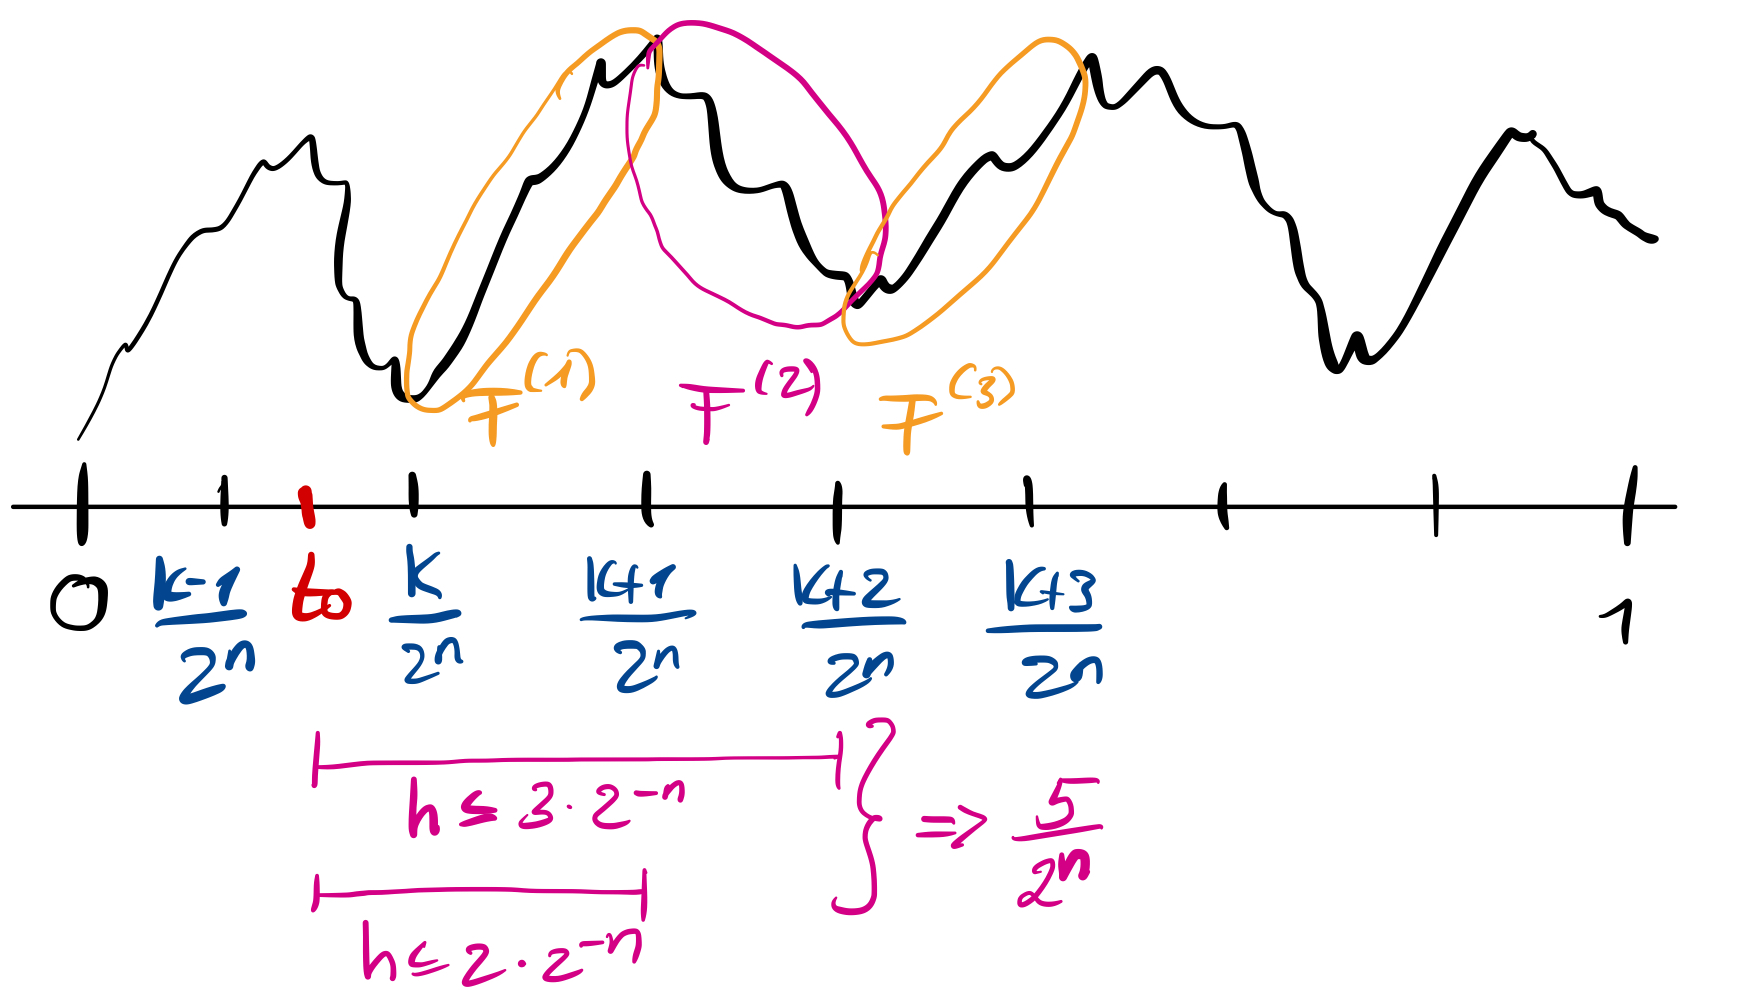
\includegraphics[scale=0.14]{diff.jpeg}
		\end{center}
	\end{figure}
	and use the triangle inequality to obtain 
	\begin{align*}
		\left\vert B_{\frac{k+1}{2^n}}(\omega) - B_{\frac{k}{2^n}}(\omega)\right\vert \overset{\triangle}&{\leq} \left\vert B_{\frac{k+1}{2^n}}(\omega) - B_{t_0}(\omega) \right\vert + \left\vert B_{t_0}(\omega) -  B_{\frac{k}{2^n}}(\omega) \right\vert \overset{\eqref{J}}{\leq} \frac{3M}{2^n},\\
		\left\vert B_{\frac{k+2}{2^n}}(\omega) - B_{\frac{k+1}{2^n}}(\omega)\right\vert \overset{\triangle}&{\leq} \left\vert B_{\frac{k+2}{2^n}}(\omega) - B_{t_0}(\omega) \right\vert + \left\vert B_{t_0}(\omega) -  B_{\frac{k+1}{2^n}}(\omega) \right\vert \overset{\eqref{J}}{\leq} \frac{5M}{2^n},\\
		\left\vert B_{\frac{k+3}{2^n}}(\omega) - B_{\frac{k+2}{2^n}}(\omega)\right\vert \overset{\triangle}&{\leq} \left\vert B_{\frac{k+3}{2^n}}(\omega) - B_{t_0}(\omega) \right\vert + \left\vert B_{t_0}(\omega) -  B_{\frac{k+2}{2^n}}(\omega) \right\vert \overset{\eqref{J}}{\leq} \frac{7M}{2^n}.
	\end{align*}
	The first inequalities implies that $\omega \in F_{n,k,M}^{(1)}$, the second $\omega \in F_{n,k,M}^{(2)}$, and the third $\omega \in F_{n,k,M}^{(3)}$.
	\begin{lstep}
		$A$ is a nullset.
	\end{lstep}
	To estimate the probability of the union we first estimate
	\begin{align*}
		\mathbb{P}\big( F_{n,k,M}^{(i)}\big) \leq \frac{7M}{2^{\frac{n}{2}}},\quad i=1,2,3.
	\end{align*}
	With $N\sim \cN(0,\frac{1}{2^n})$ and $Y\sim  \cN(0,1)$ the explicit distribution of Brownian increments and the scaling property of the standard normal distribution yield
	\begin{align*}
			 \mathbb{P}\big(F_{n,k,M}^{(3)}\big) &= \mathbb{P}\Big( \Big\vert B_{\frac{k+3}{2^n}}- B_{\frac{k+2}{2^n}} \Big\vert \leq \frac{7M}{2^n}\Big) \\
			&=\mathbb{P}\Big( \lvert N \rvert \leq \frac{7M}{2^n}\Big)\\
			 &= \mathbb{P}\Big( \lvert Y \rvert \leq \frac{7M}{2^{\frac{n}{2}}}\Big)\\
			 &= \int_{-\frac{7M}{2^{\frac{n}{2}}}}^{\frac{7M}{2^{\frac{n}{2}}}} \underbrace{\frac{1}{\sqrt{2\pi}}}_{\leq \frac{1}{2}} \underbrace{e^{-\frac{x^2}{2}}}_{\leq 1} \dint x 
			 \leq \frac{7M}{2^{\frac{n}{2}}}.
		\end{align*}
		Exactly the same estimates work for the other two probabilities (estimating $3$ and $5$ by $7$). The independence of Brownian increments shows that $F_{n,k,M}^{(1)}$, $F_{n,k,M}^{(2)}$, $F_{n,k,M}^{(3)}$ are independent. Thus, for all $n\geq 3$, we obtain
	\begin{align*}
		 \sum_{k=1}^{2^n} \mathbb{P}\big(F^n_{k,M}\big)
		 =\sum_{k=1}^{2^n} \mathbb{P}\big(F_{n,k,M}^{(1)}\big) \cdot \mathbb{P}\big(F_{n,k,M}^{(2)}\big) \cdot \mathbb{P}\big(F_{n,k,M}^{(3)}\big) 
		\leq  \sum_{k=1}^{2^n} \frac{(7M)^3}{2^{3\frac{n}{2}}} 
		=  2^n \frac{(7M)^3}{2^{3\frac{n}{2}}} = \frac{(7M)^3}{2^{\frac{n}{2}}}.
	\end{align*}
	Now define $F:=\cup_{M=1}^\infty\cap_{n=3}^\infty \cup_{k=1}^{2^n}F^n_{k,M}$. Then $A\subseteq F$, $F$ is measurable, and $\P(F)=0$ because $\P(F)\leq \sum_{M=1}^\infty \P(\cap_{n=3}^\infty \cup_{k=1}^{2^n}F^n_{k,M})$ and the inner probabilities are zero (equal to zero for all $M$, not only in the limit) as
	\begin{align*}
		\P(\cap_{n=3}^\infty \cup_{k=1}^{2^n}F^n_{k,M})\overset{\text{arbitrary $n$}}{\leq} \P(\cup_{k=1}^{2^n}F^n_{k,M})\leq \sum_{k=1}^{2^n}\P(F^n_{k,M})\leq \frac{7M}{2^{\frac{n}{2}}}.
	\end{align*}
	That's it, $t\mapsto B_t(\omega)$ is nowhere differentiable in $[0,1]$. To generalise from $[0,1]$ to $[0,\infty)$ we can repeat the same argument for $[n,n+1]$ or use the Markov property to deduce the claim for $[n,n+1]$. Since countable intersections of nullsets remain nullsets the nowhere differentiability on $[0,\infty)$ is proved.
\end{proof}
The theorem is also special as it is not so easy to construct a function that is continuous but nowhere differentiable. This is an example of the \textbf{probabilistic method}, a trick to construct an object by showing it exists as it relates to some event of some probability space with positive probability.\smallskip

There are many, many more properties known for the Brownian sample paths. We are going to stop here, so take the chance to summarize in a drawing everything you learned about the Brownian sample paths!
\begin{figure}[h]
	\begin{center}
		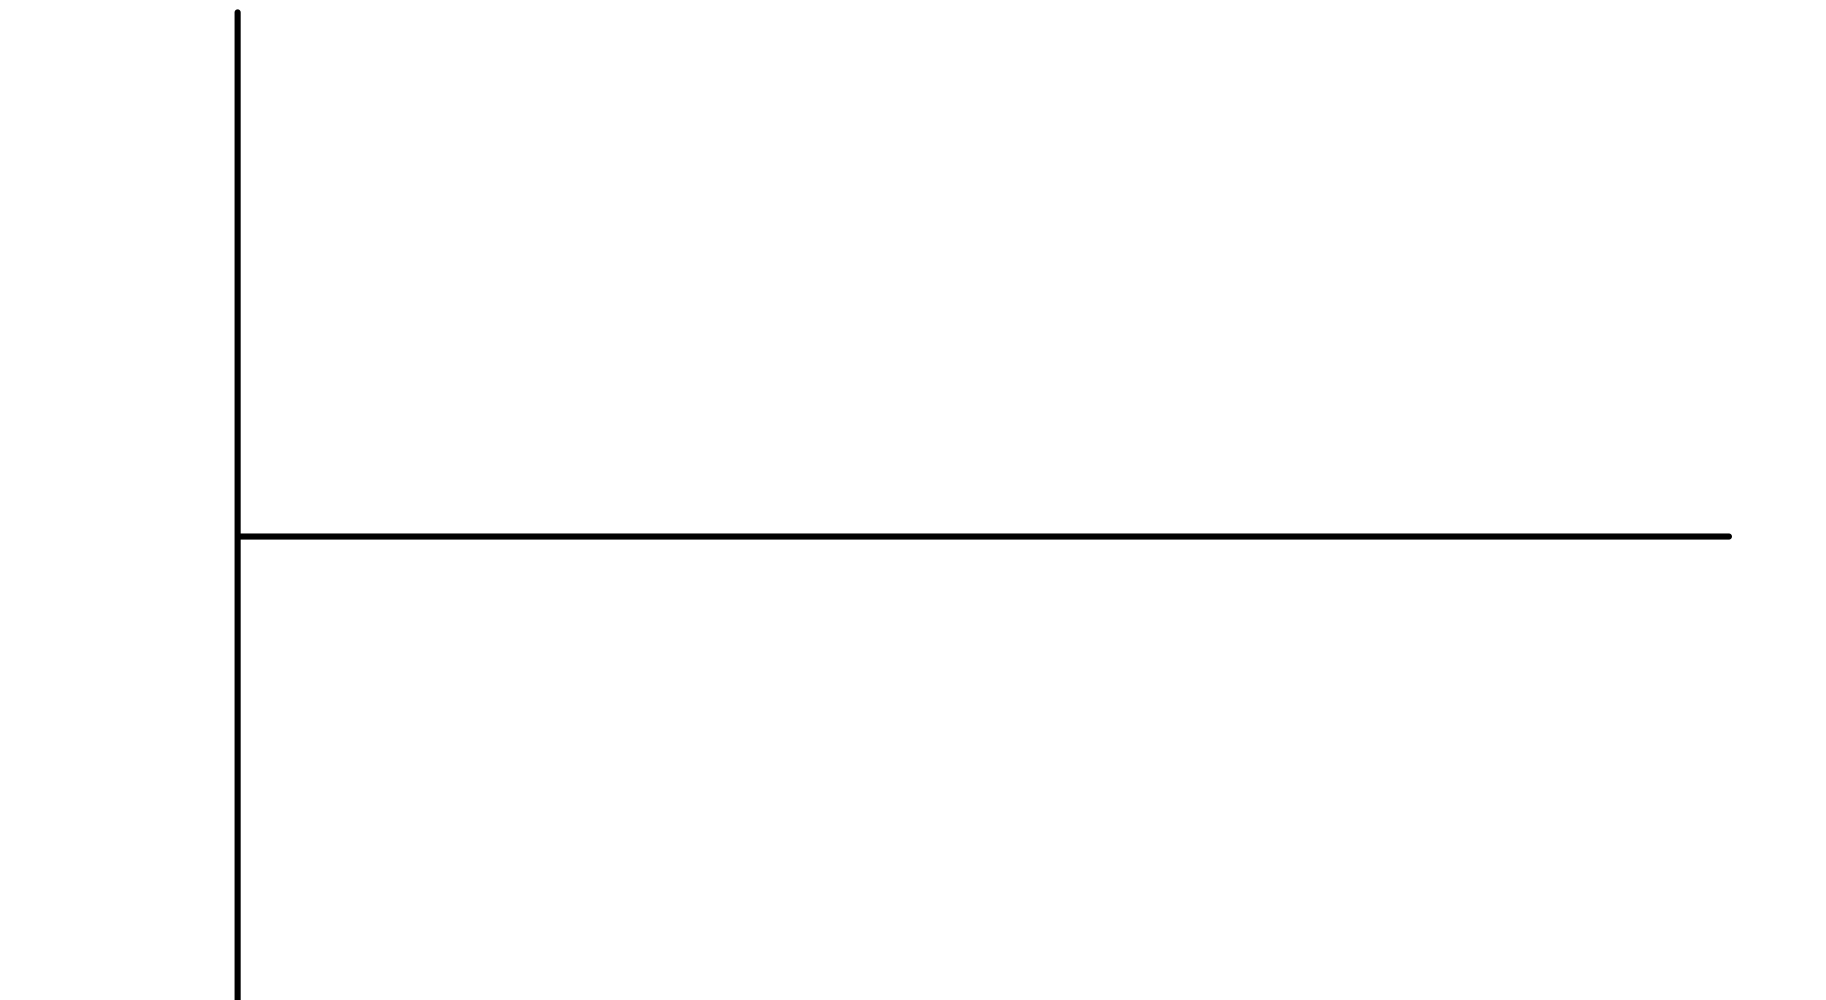
\includegraphics[scale=0.1]{BrownianBild.jpeg}
	\end{center}
\end{figure}
\section{Weak convergence of continuous stochastic processes}
One of the most fundamental features of the Brownian motion is the universal approximation property through random walks. We will prove below that scaled random walks converge towards the Brownian motion if time and space are scaled appropriately towards the continuum. But what does convergence mean? As a picture of course something like "the paths looks similar"{} but what is a good notion of convergence? As for random variables there are different notions of convergence, we stick to weak convergence of laws. To use results from Chapter \ref{chapter:CV} (most importantly Prohorov's theorem) a sequence of stochastic processes must be interpreted as a sequence of path-valued random variables with a Polish path-space. The generic path-space $\R^{[0,\infty)}$ fulfills the first property (Proposition \ref{zweiInterprb}) but carries no topological structure. If the stochastic processes are continuous, then they are $C([0,\infty))$-valued random variables (see the discussion above Definition \ref{def:claw}) and the path-space is Polish by Proposition \ref{prop:C}. Then we can define the weak convergence of $X^n$ to $X$ as weak convergence of $\P^{X^n,c}$ to $\P^{X,c}$ on $\mathcal B(C([0,\infty)))$, and that is what we are going to do. There is only a small detail. If proceesses are only continuous almost surely then we will always modify them to be the constant zero-function away from the event of probability $1$ on which path are continuous. Since modifications have same finite-dimensional martingals (and same law) this detail never poses a problem and can freely be ignored.
\begin{lwarnhinweis}
	From now on we will skip the superscript $c$ from the law $\P^{X,c}$ of an (almost surely) continuous process on $\mathcal B(C([0,\infty)))$.
\end{lwarnhinweis}
Before defining weak convergence of continuous processes as weak convergence of their laws let us apply the general theory to understand the weak convergence of probability measures on the path-space of continuous functions.
\begin{laussagewerkzeug}
	\begin{prop}\label{most_useful_characterization_weak_convergence_C}
		Let $\mu,\mu^1, \mu^2, ...$ a sequence of probability measures on $\mathcal B(C([0,\infty))$. Then $\mu^n\overset{\text{(w)}}{\rightarrow} \mu$, $n\to\infty$, is equivalent to
		\begin{enumerate}[label=(\roman*)]
				\item $\{\mu^n:n\in\N\}$ is tight in $\mathcal M_1(C([0,\infty)))$,
				\item All finite-dimensional distributions converge, i.e. 
				\begin{align*}
					\mu^n_J=\mu^n \circ \pi^{-1}_J\overset{\text{(w)}}{\longrightarrow} \mu \circ \pi^{-1}_J=\mu_J,\quad n\to\infty,
				\end{align*}
				for all finite $J\subseteq [0,\infty)$.
			\end{enumerate}
	\end{prop}
	\end{laussagewerkzeug}
\begin{proof}[Proof]
	The claim follows from Proposition \ref{propkonvergenz}.\smallskip
	
	"$\Rightarrow$": Proposition \ref{propkonvergenz} and Prohorov's theorem yield (i). Continuous mapping (Theorem \ref{thm:continuousmapping}) yields (ii) as all projections are continuous mappings.\smallskip

	"$\Leftarrow$": (i) implies the relative sequential compactness (Prohorov's theorem). Next suppose $(\mu^{n_k})$ is any converging subsequence with some weak limit $\bar \mu$. Then (again by continuous mapping) all finite-dimensional distributions of $(\mu^{n_k})$ converge to those of $\bar \mu$. Since, by assumption, the finite-dimensional distributions also converge to those of $\bar\mu$ this implies that $\bar \mu$ and $\mu$ have the same finite-dimensional marginal distributions, thus, using Proposition \ref{prop:uniqueC}, $\bar \mu=\mu$.
\end{proof}	
Going through Chapter \ref{chapter:CV} one might ask why the proposition was not deduced from Proposition \ref{most_useful_characterization_weak_convergence} which was used to characterise weak convergence on $[a,b], [0,\infty)$, and $\R^d$. The reason is simple. The projections $\pi_J$ are continuous but not bounded, in contrast to $x^n$ on $[a,b]$, $\exp(-\lambda x)$ on $[0,\infty]$, and $e^{i\langle t,x\rangle}$ on $\R^d$. That's why we directly argue with Proposition \ref{propkonvergenz} and the continuous mapping theorem.\smallskip

As usuallly we are mostly interested in the stochastic reformulation, not in abstract measure theory. As for random variables and random vectors in Chapter \ref{chapter:CV} the reformulation is immediate by defining the weak convergence of continuous processes as the weak convergence of their laws.
\begin{ldef}
\begin{deff}\label{def:wk}
	Suppose $X,X^1,X^2,...$ are stochastic processes with almost surely continuous paths and laws $\mathbb{P}^{X},\mathbb{P}^{X^1},...$ on $C([0,\infty))$.
	\begin{enumerate}[label=(\roman*)]
		\item $(X^n)_{n\in\N}$ is said to \textbf{converge weakly to $X$} if $\mathbb{P}_{X^n} \overset{\text{(w)}}{\longrightarrow} \mathbb{P}_X$, $n\to\infty$. In that case we write $X^n \Rightarrow X$.%, but also $X^n \overset{\text{(w)}}{\rightarrow} X$ or $X^n \overset{\text{(d)}}{\rightarrow} X$.
		\item The \textbf{finite-dimensional distributions (fdds)} of $(X^n)_{n\in\N}$ converge to those of $X$ if for all choices $0 \leq t_1 \leq ... \leq t_k$
		\begin{align*}
			\left( X_{t_1}^n,...,X_{t_k}^n \right) \overset{\text{(d)}}{\longrightarrow} \left( X_{t_1},...,X_{t_k}\right), \quad n\to\infty,
		\end{align*}
		or, equivalently,
		\begin{align}
			\P^{X^n}_{t_1,...,t_k}\overset{\text{(w)}}{\longrightarrow} \P^X_{t_1,...,t_k},\quad n\to\infty.
		\end{align}
		In that case we write $X^n \overset{\text{fdd}}{\Longrightarrow}X$.
	\end{enumerate}
\end{deff}
\end{ldef}
It is easy to see how the two concepts relate to each other: Since $(X_{t_1}^n,...,X_{t_k}^n) = \pi_{t_1,...,t_k}(X^n)$ and projections are continuous the continuous mapping theorem (more precisely the discussion below) yields
	\begin{align*}
		X^n \Rightarrow X,\quad n\to\infty\quad  \Longrightarrow \quad X^n \overset{\text{fdd}}{\Longrightarrow}X,\quad n\to\infty.
	\end{align*}
	The converse is usually not true. The finite-dimensional distributions do not contain enough information, for instance on continuity. It may happen that the finite-dimensional distributions of a sequence of continuous processes converge to those of a discontinuous process and weak convergence does not hold. Nonetheless, it is reasonable to ask why we aim at proving the stronger weak convergence instead of fdd convergence. The answer is similar to the different modes of convergence of random variables. We always aim for the strongest notion if possible, as extra features might be useful. Here, the big advantage is the continuous mapping theorem as weak convergence implies $F(X^n)\overset{(d)}{\rightarrow} F(X)$ for any continuous mapping $F:C([0,\infty))\to \R$ whereas fdd convergence only implies $F(X^n_{t_1},..., X^n_{t_k})\overset{(d)}{\rightarrow} F(X_{t_1},..., X_{t_k})$ for continuous $F:\R^k\to \R$. For example, weak convergence automatically implies $$\int_0^1 X_s\dint s\overset{\text{(d)}}{\longrightarrow}\int_0^1 X_s\dint s\quad \text{and}\quad \sup_{t\leq T}|X_t^n|\overset{(d)}{\longrightarrow} \sup_{t\leq T}X_t.$$ If fdd convergence holds and additionally the sequence is tight then weak convergence holds:
	\begin{lAussageWerkzeug}
\begin{theorem}
	A sequence $(X^n)_{n\in\N}$ of continuous stochatic processes converges weakly to $X$ if and only if  
	\begin{enumerate}[label=(\roman*)]
		\item $\{\P^{X^n}:n\in\N\}$ is tight in $\mathcal M_1(C([0,\infty)))$,
		\item $X^n \overset{\text{fdd}}{\Longrightarrow}X$, $n\to\infty$.
	\end{enumerate}
\end{theorem}
\end{lAussageWerkzeug}
Convergence of finite-dimensional distributions is nothing but weak convergence of random vectors, the topic of Section \ref{sec:WC}. All the tools, most importantly convergence of characteristic functions, have already been established. Here is an example which is particularly simple. For centered Gaussian processes (and only Gaussian processes!) only the two-dimensional marginal distribution have to converge and those are characterised by the covariance function. 
\begin{luebung}
	If $X, X_1, X_2,...$ are Gaussian processes with covariance functions $K, K^1, K^2,...$, then $X^n \overset{\text{fdd}}{\Longrightarrow}X$ if and only if $\lim_{n\to\infty}K^n(t,s)=K(t,s)$ for all $t,s\in I$.
\end{luebung}
The remaining task is how to check tightness in $C([0,\infty))$. Recalling the general definition
\begin{align*}
	\forall \varepsilon > 0 \: \exists K \subseteq E \text{ compact}\colon \: \mu^n(K^c) < \varepsilon \quad \forall n \in \N,
\end{align*}
it is clear that we need to discuss compact sets in $(C([0,\infty),d)$. In lectures on functional analysis the study of compactness (or relative compactness) is central, the fundamental theorem is the Arz\'ela-Ascoli theorem. Recall that a set $A$ is compact if all sequences have a subsequence that converges in $A$, $A$ is called relatively compact if all sequences have a convergent subsequences but the limit must not belong to $A$ (it automatically belongs to $\bar A$). The Arz\'ela-Ascoli theorem states that $A \subseteq C([0,\infty))$ is relatively compact if and only if 
	\begin{enumerate}[label=(\roman*)]
		\item $\big\{ f(0)\colon f\in A\big\} \subseteq \R$ is bounded
		\item $\lim_{\delta \to 0} \sup_{f\in A} V_f^N(\delta) = 0 $ for all $N \in \N$, where $$V_f^N(\delta) = \sup_{\lvert t - s \rvert < \delta, \: t,s \leq N} \lvert f(t)- f(s) \rvert$$ is the so-called modulus of continuity.
	\end{enumerate}
Most courses on probability translate the theorem in order to give an if and only if condition for weak convergence of continuous processes. As this is rarely used we take a drastic detour by only considering examples that help to understand compactness in $C([0,\infty))$ and then restrict ourselves to the main example of interset for probabilists - functions that are H\"older continuous on compacts. In simple words Arz\'ela-Ascoli tells us that only two things can go wrong to make a set $A$ not (relatively) compact:
\begin{itemize}
	\item functions in $A$ are not sufficiently bounded,
 	\item there are regularity holes (like $\Q$ are holes in $\R$, just more complicated), not all functions in $A$ have the same kind (measured in terms of the modulus of continuity) of regularity.
\end{itemize}
Comparing to compact sets in $\R$ this is roughly boundedness and closedness, at least it gives the right intuition. Let's have a look at some examples:
\begin{example}
	\begin{enumerate}[label=(\roman*)]
		\item Singleton sets $A \coloneqq \{ f \}$ are compact.
		\item $A \coloneqq \{ \text{all constant functions}\}$ are not compact but all constant functions bounded by some constant $C$ are compact.
		\item Here are three examples where regularity but not boundedness is the problem. The families $f_n$ and $h_n$ should be clear from the drawing, $g_n$ is defined by
		$$g_n(x) = \begin{cases}
			x^{\frac{1}{n}} &: x \leq 1 \\
			2-x &: x\in (1,2) \\
			0 &: x\geq 1
		\end{cases}.$$
		\begin{figure}[h]
			\begin{center}
				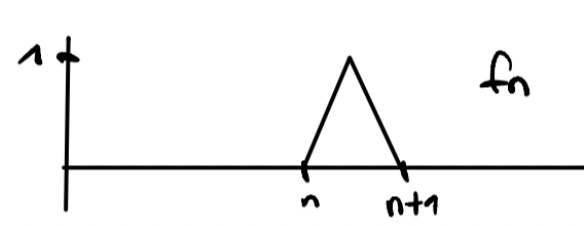
\includegraphics[scale=0.2]{compact1.jpeg}
				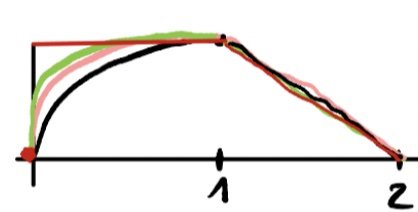
\includegraphics[scale=0.2]{compact2.jpeg}
				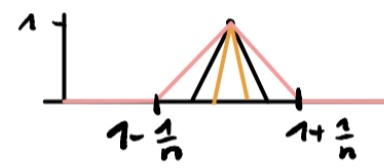
\includegraphics[scale=0.2]{compact3.jpeg}
				\caption*{Examples where regularity can get lost}
			\end{center}
		\end{figure}
		The set $A=\{f_n:n\in\N\}$ is not compact, there are sequences that converge to the zero-function which is not in $A$ (recall from Proposition \ref{prop:C} that convergence in $C([0,\infty))$ is uniform convergence on compacts). Since the zero-function is continuous the limit of all subsequences is at least in $C([0,\infty))$, hence, $A$ is not compact but  relatively compact. The set $B=\{g_n:n\in\N\}$ is neither compact nor relatively compact as sequences in $B$ might converge uniformly to $f=\mathbf 1_{\{0\}}$ which is not in $C([0,\infty))$. The same holds for the final example where sequences can converge uniformly on compacts to $\mathbf 1_{\{1\}}$ which is not in $C([0,\infty))$.
	\end{enumerate}
\end{example}
What goes wrong in the examples? Boundedness or regularity. So far we have measured regularity in terms of H\"older continuity. The examples are made up from examples that do not have the same index of H\"older continuity. This leads us to the most important examples of compact sets of continuous functions:

\begin{laussagewerkzeug}
	\begin{lemma}\label{ohmann}
		Suppose $(K_N)_{N\in\N}$ are non-negative and $\gamma\in (0,1]$. Then
		\begin{align*}
			 A^\gamma_{K}
			&:=\big\{f:[0,\infty)\to \R\,\big|\, f\text{ is H\"older continuous on compacts with index $\gamma$ and}\\
			&\qquad\qquad\qquad \quad\qquad \text{ constants $K_N$ and } |f(0)|\leq K_0\}
		\end{align*}
		is compact in $C([0,\infty))$.
	\end{lemma}
\end{laussagewerkzeug}
\begin{proof}[Proof]
	This follows directly from Arz\'ela-Ascoli. The boundedness condition holds by definition and the regularity condition follows from the H\"older continuity:
	\begin{align*}
		V_f^N(\delta) = \sup_{\lvert t-s \rvert < \delta,\: t,s\leq N} \lvert f(t)- f(s) \rvert \leq K_N \cdot \sup_{\lvert t-s \rvert < \delta,\: t,s\leq N} \lvert t-s\rvert^{\gamma} = K_N \cdot \delta^{\gamma},
	\end{align*} 
	which uniformly converges to $0$ as $\delta\to 0$ as the right hands side is independent of $f\in A^\gamma_K$. Hence, the set $A^\gamma_K$ is relatively compact. In fact, such sets are automatically compact as H\"older continuity transfers to limits. Suppose $(f_n)$ is a converging sequence with $f_n\to f$, $n\to\infty$, then, if $t,s\leq N$,
	\begin{align}
		|f(t)-f(s)|=\lim_{n\to\infty}|f_n(t)-f_n(s)|\leq \lim_{n\to\infty} K_N|t-s|^\gamma=K_N|t-s|^\gamma,
	\end{align}
	because uniform convergence also implies pointwise convergence. Hence, the H\"older continuity on $[0,N]$ is inherited by the limit so that $f$ is H\"older continuous on compacts.
\end{proof}
In essence, this is all we need from functional analysis! The lemma and the following theorem motivates why we introduced the notion of H\"older continuity on compacts for these lecture notes, the notion allows us to work out very clearly what is going on. 
\begin{luebung}
	Check yourself where the previous proof breakes down if H\"older continuous on compacts is replaced by locally H\"older continuous.
\end{luebung}
The next step is to use the previous lemma to provide a simple tightness criterion for continuous processes. The Kolmogorov-Chentsov condition reappears, which is little surpising as under that condition sample paths are H\"older continuous. Unfortunately, there is a very delicate detail involved. According to Kolmogorov-Chentsov sample paths are only locally H\"older continuous, what is needed to apply Lemma \ref{ohmann} is H\"older continuity on compacts. A very close look at the proof of Kolmogorov-Chentsov safes us, the Kolmogorov-Chentsov condition is enough to have paths that are H\"older continuous on compacts, but only with probability close to $1$. Luckily, this is enough for the definition of tightness.
\marginpar{\textcolor{red}{Lecture 26}}

\begin{lAussageWerkzeug}
\begin{theorem}[Kolmogorov-Chentsov tightness criterion]\label{thm:KolTightness}
	Suppose $(X^n)_{n\in\N}$ is a sequence of continuous stochastic processes on $(\Omega,\cA,\mathbb{P})$ such that
	\begin{enumerate}[label=(\roman*)]
		\item $(\P^{X_0^n})_{n\in\N}$ is tight in $\mathcal M_1(\R)$,
  		\item for all $n\in\N$ and $T>0$ there are $c, \alpha$, $\beta$ (independent of n!) with
	  \begin{align*}
		  \E\big[\lvert X_t^n - X_s^n \rvert^{\alpha}\big] \leq c \cdot \lvert t - s \rvert^{1+\beta},\quad \forall t,s \leq T.
  	\end{align*}
	\end{enumerate}
	Then $(\P^{X^n})_{n\in\N}$ is tight in $\mathcal M_1(C([0,\infty)))$.
\end{theorem}
\end{lAussageWerkzeug}
There is no reason to worry much about (i), in most applications $X_0^n$ is indepenent of $n$ so that (i) is always satisfied. The interesting condition is (ii). Luckily the form of (ii) can be checked in many situations (such as for Donsker's theorem below)!
\begin{proof}[Proof]
	For the proof we first refine the proof of the Kolmogorov-Chentsov Theorem \ref{thm:chentsov}. This could have been done straight in the Komogorov-Chentsov proof. Since the refinement is only needed here we kept Kolmogorov-Chentsov a little easier. Recall from the remark below the proof of Theorem \ref{thm:chentsov} that $\tilde X$ and $X$ are indistinguishable because $X$ is assumed continuous. Hence, the proof gives information on the paths of $X$ rather than constructing a modification. With arbitrary $\gamma<\frac{\beta}{\alpha}$ the following refinement holds under the assumptions of Theorem \ref{thm:chentsov}:
	\begin{lstep}
		For all $\varepsilon>0$ there are a non-negative constants $(K_N)_{N\in \N}$ such that
		\begin{align*}
			\P\big(\text{$X$ is H\"older continuous on compacts with index $\gamma$ and constants $K_N$}\big)>1-\varepsilon.
		\end{align*}
		The constants $K_N$ and $\gamma$ only depend on $\varepsilon, \alpha, \beta, $ and $c$.
	\end{lstep}
	Recall that H\"older continuity on compacts lies between globally and locally H\"older continuous. We prove a slightly stronger statement on the paths, but lose a bit of probabiity. To see what needs to be proved let us first clarify the difference between this claim and the statement of Kolmogorov-Chentsov. In Kolmogorov-Chentsov we proved that there are (random) neighborhoods $U_t(\omega)=(t-2^{-n_0(\omega)}, t+2^{-n_0(\omega)})$ such that $|X_t(\omega)-X_s(\omega))|\leq K|t-s|^\gamma$ for all $s\in U_t(\omega)$. Here, we claim that the estimate holds for all $t,s\leq N$ at once. This is not global H\"older continuity on $[0,\infty)$ for which the estimate should hold for all $t,s\geq 0$.\smallskip

	It is best to see the refinement as an occasion to once more browse through the delicate Kolmogorov-Chentsov proof, we use the definitions from that proof. Defining $B_N =\cup_{k=N}^\infty A_k$, the proof showed that, chosing $N$ large enough, 
	\begin{align*}	
		\P(B_N)\leq \sum_{k=N}^\infty \P(A_k)\leq c \sum_{k=N}^\infty 2^{-k(\beta - \alpha  \gamma)} \leq \varepsilon.
	\end{align*}
	Then, for all $\omega\notin B_N$ (for these $\omega$ all dyadic increments with $2^{-n}<2^{-N}$ are under control), the chaining argument shows that the H\"older estimate $|X_t(\omega)-X_s(\omega)|\leq K|t-s|^\gamma$ holds whenever $|t-s|<\delta:=2^{-N}$. Here lies the crucial difference. For Kolmogorov-Chentsov we aimed to prove an almost sure statement, but we allowed ourselves to take different $N$ for different $\omega$. Borel-Cantelli was used to ensure that almost all $\omega$ lie in some of the $B_n$ and for that $\omega$ we worked with the corresponding $n$. Here we want the same $N$ for all $\omega$ but accept a statement with probability $1-\varepsilon$. In contrast to the Kolmogorov-Chentsov proof the sizes of the neighborhoods $U_t(\omega)$ are now indepenent of $\omega$, we can chose $(t-2^{-N},t+2^{-N})$, but still the H\"older estimate does not hold for all $s,t\leq N$. We are luckily in a situation in which the H\"older constants are the same in all neighborhoods (they are $K := \frac{2}{1-2^{-\gamma}}$). This allows us to use a trick for H\"older continuous functions. If $f$ is locally H\"older continuous with $|f(t)-f(s)|\leq K|t-s|^\gamma$ for all $|t-s|<\delta$, then $f$ is actually nearly H\"older continuous! This follows from a telescopic sum and the triangle inequality. Setting $n:=\lceil\frac{N}{\delta}\rceil$, chaining forwards from $s$ to $t$ yields
	\begin{align*}
		|f(t)-f(s)|\leq \sum_{k=1}^n \Big|\Big(f\Big(s+(t-s)\frac{k}{n}\Big)-f\Big(s+(t-s)\frac{k-1}{n}\Big)\Big|\leq K \sum_{k=1}^n \Big|\frac{t-s}{n}\Big|^\gamma=K_N|t-s|^\gamma,
	\end{align*}
	for all $s,t\leq N$, with the new constant $K_N:=K n^{1-\gamma}$. Hence, for all $\omega\notin B_n$, the sample paths are H\"older continuous on compacts with the same index and constants.
	\begin{lstep}
		The sequence $(\P^{X^n})_{n\in\N}$ is tight in $\mathcal M_1(C([0,\infty)))$.
	\end{lstep}
	Fix $\varepsilon>0$ and chose a constant $K$ such that $\sup_{n\in\N}\P(|X^n_0|>K)=\sup_{n\in\N}\P^{X_0^n}([-K,K]^c)<\frac{\varepsilon}{2}$. Next, fix $\gamma<\frac{\beta}{\alpha}$ and apply the previous step to all $X^n$ with $\frac{\varepsilon}{2}$. This yields constants $(K^{\varepsilon}_N)_{N\in\N}$ (the same constants work for all $n$) such that $X^n$ is H\"older continuous on compacts with index $\gamma>0$ and constants $(K_N)_{N\in\N}$ with probability $1-\frac{\varepsilon}{2}$. In other words, $\sup_{n\in\N}\P^{X^n}(A^\gamma_{K^\varepsilon})\geq 1-\varepsilon$ with the compact sets $A^\gamma_{K^\varepsilon}$ from Lemma \ref{ohmann}. But then the tightness is proved.
\end{proof}
\section{Donsker's Theorem}
All ingredients have been collected to prove one of the most important theorems on stochastic processes. Just as the standard normal distribution is the universal (weak) limit of scaled sums the Brownian is the universal (weak) limit of scaled random walks. Of course there is no surprise, random walks are based on sums of iid random variables! The theorem can be seen as an infinite-dimensional (path-valued) analogue of the central limit theorem and as such is called a functional central limit theorem. \smallskip

To understand the theorem first recall the definition of a simple random walk from Example \ref{ex:RW}. If $Y_1,Y_2,...$ are iid on $(\Omega,\cA,\mathbb{P})$, then $S_k \coloneqq \sum_{i=1}^k Y_i$ is called a random walk. Since a Brownian motion is defined in continuous time we extend the random walk to continuous time by linear interpolation, recall Example \ref{conta}. The piecewise-linear interpolation $X$ is a continuous stochastic process on $(\Omega,\cA,\mathbb{P})$. To turn a simple random walk into a Brownian motion the jump frequency is increased to $n$ jumps per time-unit, and again linearly interpolated. In a drawing the time-scaling is easily understood, the formal definition will be bit unhandy.
\begin{figure}[h]
	\begin{center}
		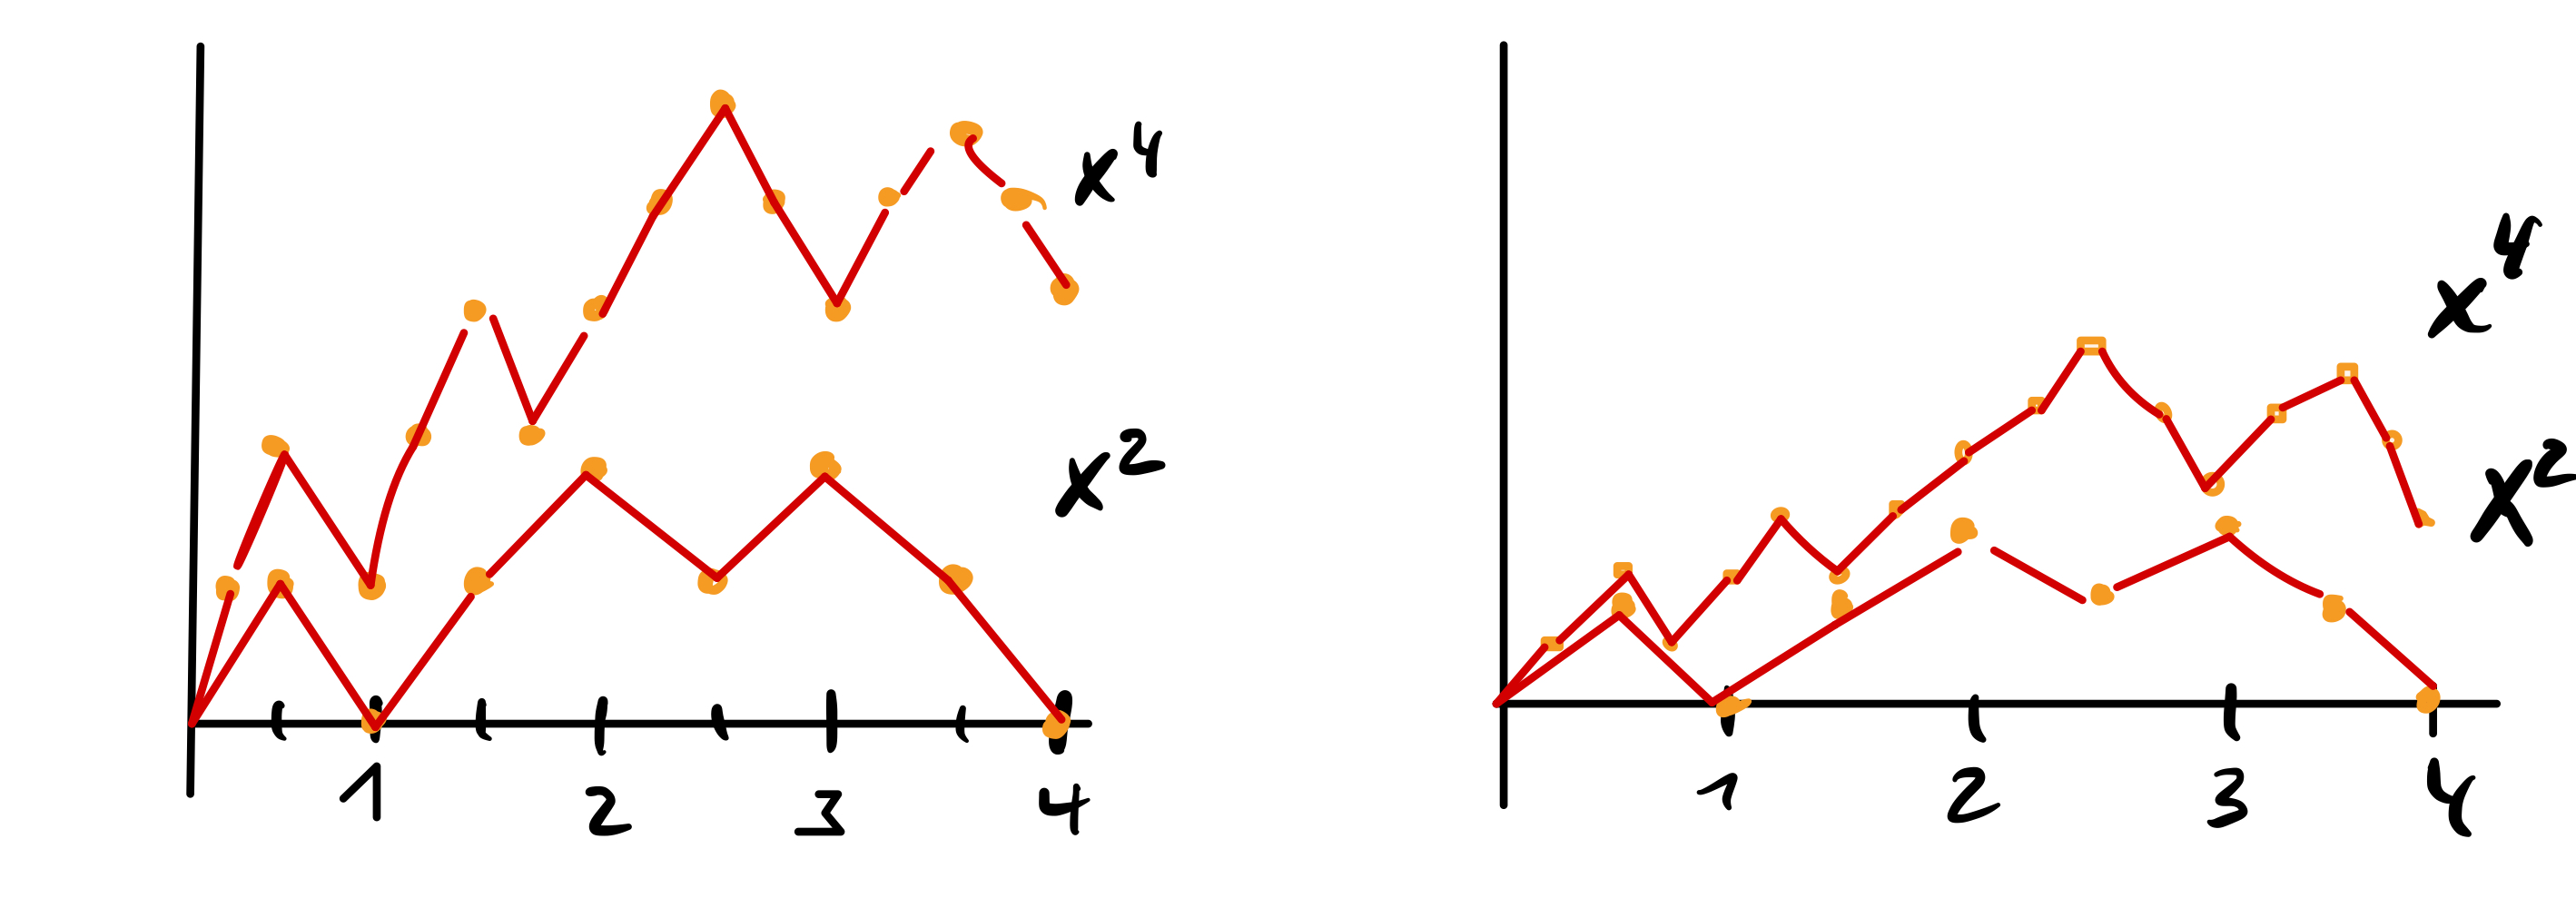
\includegraphics[scale=0.13]{scaling2.jpeg}
	\end{center}
	\caption*{Without spatial scaling on the left, with spatial scaling on the right}
	\end{figure}

If we only speed-up in time then we cannot send $n$ to infinity as trajectories will tend to diverge. More formally, at time $1$ the process is the sum of $n$ independent random variables which for large $n$ we understand well from the law of large numbers and the central limit theorem. If the sum is additionally multiplied by $\frac{1}{n}$ then, almost surely, the process at time $1$ (and all other integers) will converge to $\E[Y_1]=0$. Hence, also the linear interpolation vanishes in the limit, the multiplication by $\frac{1}{n}$ is too extrem. What is more interesting is to multiply the sum by $\frac{1}{\sqrt{\sigma n}}$ if $\sigma^2=\Var[Y_1]$ as now the central limit theorem gives convergence in distribution to $\mathcal N(0,1)$. Donsker's theorem is the process version of this observation for a one-dimensional marginal. If the speed-up random walk trajectory is multiplied by $\frac{1}{\sqrt{\sigma n}}$ then (weak) convergence towards the Brownian motion holds. 
\begin{laufmerksamkeit}
	In probability theory such a procedure is called scaling, and a scaling which speeds up linearly in time and square-root like in space is called \textbf{Brownian scaling} because it leads to the Brownian limit. 
\end{laufmerksamkeit}
To state and prove Donsker's theorem a formal definition of the linearly-interpolated scaled random walks is needed. First define the constantly interpolated scaled random walk by
	\begin{align*}
		\tilde{X}_t^n \coloneqq \frac{\sum\limits_{k=1}^{\lfloor nt \rfloor}\left( Y_k - \E[Y_1]\right)}{\sigma \sqrt{n}}, \quad t\geq 0,
	\end{align*}
	where $\lfloor x \rfloor = \sup\{ n\in\N\colon n \leq x\}$,	and from this the linearly interpolated scaled random walks by adding linear pieces with the appropriate slopes:
	\begin{align*}
		X_t^n \coloneqq \tilde{X}_t^n + (nt - \lfloor nt \rfloor ) \frac{Y_{\lfloor nt \rfloor + 1}-\E[Y_1]}{\sigma \sqrt{n}} ,\quad t\geq 0.
	\end{align*}
	\begin{figure}[h]
		\begin{center}
			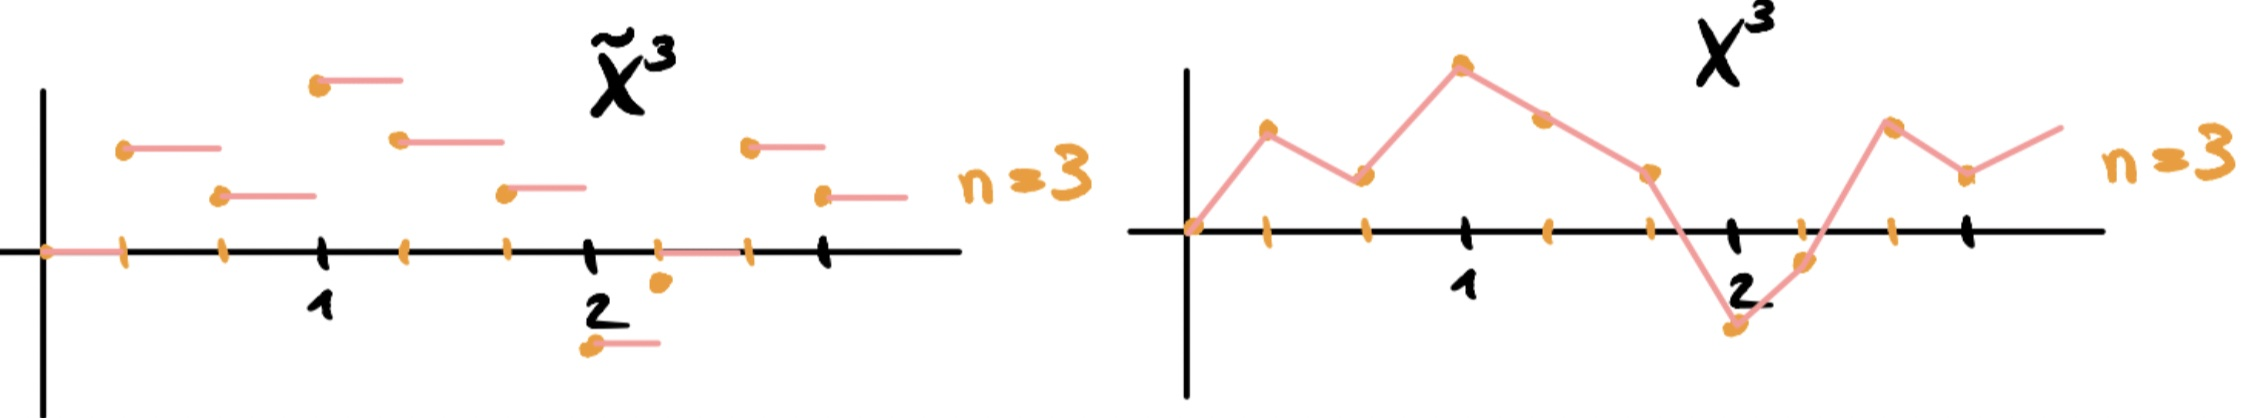
\includegraphics[scale=0.13]{RWs.jpeg}
		\end{center}
		\end{figure}
		The formula is much more unsightly than it's content, just try yourself to write down a formula that linearly interpolates values on $\N$ and you will quickly derive the formula yourself!
\begin{lSatzHerz}
\begin{theorem}[Donsker functional CLT]\label{thm:donsker}
	If $\sigma^2 = \mathbb{V}[Y_1]<\infty$, then $X^n \Rightarrow B$, $n\to\infty$, where $B$ is a Brownian motion.\smallskip

	In other words: The rescaled random walk measures converge weakly on $\mathcal B(C([0,\infty)))$ to the Wiener measures.
\end{theorem}
\end{lSatzHerz}
Since the theorem only depends on the variance (not on the entire distribution) the theorem is also called \textbf{Donsker's invariance principle}, the Brownian motion is the universal scaling limit of \underline{all} random walks with finite second moment jump sizes, just like the central limit theorem is the universal limit of scaled sums of all iid random variables with finite second moments.
\begin{proof}[Proof]
	Just as in the proof of the central limit theorem it can be assumed without loss of generality that $\E[Y_1]=0$ and $\sigma^2=1$. Otherwise the claim is deduced from normalizing $\tilde Y_1:= \frac{Y_1-\E[Y_1]}{\sigma}$. To prove weak convergence we use the theory of the previous section and prove convergence of finite-dimensional distributions and tightness.
	\begin{lstep}
		$X^n \overset{\text{fdd}}{\Longrightarrow} B$, $n\to\infty$
	\end{lstep}
	Recall from Definition \ref{def:wk} that we need to prove the (finite-dimensional) convergence
	\begin{align}
		(X_{t_1}^n,..., X_{t_k}^n)\overset{\text{(d)}}{\rightarrow}(B_{t_1},..., B_{t_k}) ,\quad n\to\infty,
	\end{align}
	for all $0\leq t_1\leq...\leq t_k$. First note that, for $s\leq t$, the central limit theorem implies
			\begin{align*}
				\tilde{X}_t^n - \tilde{X}_s^n = \frac{\sum\limits_{k= \lfloor ns \rfloor + 1 }^{\lfloor nt \rfloor}Y_k}{\sqrt{n}} \overset{\text{(d)}}{=} \frac{\sum\limits_{k= 1}^{\lfloor n(t-s) \rfloor}Y_k}{\sqrt{n}} \overset{\text{(d)}}{\longrightarrow} \cN(0,t-s),\quad n\to\infty.
			\end{align*}
			Since, for $0\leq t_1 \leq ... \leq t_k$, the sums $\tilde{X}_{t_2}^n - \tilde{X}_{t_1}^n, \dots , \tilde{X}_{t_k}^n - \tilde{X}_{t_{k-1}}^n$ are independent (sums over different $Y$), it follows that, for some Brownian motion $B$,
			\begin{align*}
				\left(\tilde{X}_{t_2}^n - \tilde{X}_{t_1}^n, \dots , \tilde{X}_{t_k}^n - \tilde{X}_{t_{k-1}}^n \right) \overset{\text{(d)}}{\longrightarrow} \left( B_{t_2}-B_{t_1}, \dots , B_{t_k} - B_{t_{k-1}}\right).
			\end{align*}
			We already used the trick of rewriting a vector as a matrix multiplied to a vector of incremets (compare the proof of Proposition \ref{BMGaussian}). Using the trick again and noting that $f(x) = A \cdot x$ is continuous, the continuous mapping theorem \ref{thm:continuousmapping} yields
			\begin{align*}
				\left(\tilde{X}_{t_1}^n,\dots , \tilde{X}_{t_k}^n\right) \overset{\text{(d)}}{\longrightarrow} \left( B_{t_1},\dots , B_{t_k}\right),\quad n\to\infty.
			\end{align*}
			This shows the weak convergence $\tilde{X}^n \overset{\text{fdd}}{\Longrightarrow} B$, $n\to\infty$, for the constant interpolation. To get convergence of finite-dimensional distributions for the linear interpolation one of the many formulations of \textbf{Slutsky's lemma} is used:
			\begin{laufmerksamkeit}
					If $(X_n)$ and $(Y_n)$ are two sequences of random vectors such that
					$X_n \overset{\text{(d)}}{\to} X$ and $|X_{n,k}-Y_{n,k}| \overset{\text{P}}{\to} 0$ for all coordinates $k$, then $Y_n \overset{\text{(d)}}{\to} X$.
			\end{laufmerksamkeit}
			First note that $|X_{n,k}-Y_{n,k}| \overset{\text{P}}{\to} 0$ for all $k$ also implies $|X_{n}-Y_{n}| \overset{\text{P}}{\to} 0$, because
			\begin{align*}
				\P(|X_n-Y_n|>\varepsilon)\leq \P(\cup_{k=1}^d\{|X_{n,k}-Y_{n,}|\geq \varepsilon/d\})\leq \sum_{k=1}^d \P(|X_{n,k}-Y_{n,k}|>\varepsilon/d)\to 0,\quad n\to\infty.
			\end{align*}
			Then we can estimate, for $f$ bounded Lipschitz continuous with Lipschitz constant $K$ and $\varepsilon>0$,
			\begin{align*}
				&\quad \lim_{n\to\infty}\big|\E[f(Y_n)]-\E[f(X)]\big|\\
				\overset{\Delta}&{\leq} 	\lim_{n\to\infty} \E[|f(Y_n)-f(X_n)|]+\underbrace{\lim_{n\to\infty}\big|\E[f(X_n)]-\E[f(X)]\big|}_{=0}\\
				&\leq  	\lim_{n\to\infty} \big(\E[|f(Y_n)-f(X_n)|\mathbf 1_{|Y_n-X_n|>\varepsilon}]+\E[|f(Y_n)-f(X_n)|\mathbf 1_{|Y_n-X_n|\leq \varepsilon}]\big)\\
				\overset{\Delta,\text{ $f$ bounded, $f$ Lip.}}&{\leq}  	\lim_{n\to\infty} 2||f||_\infty \P(|Y_n-X_n|>\varepsilon)+K\varepsilon=K\varepsilon.
			\end{align*}
			Since $\varepsilon$ is arbitrary, the lefthand side equals $0$. Portemanteau \ref{portemanteau} then implies the weak convergence, $f$ Lipschitz is enough.\smallskip
			
			
			
			
			
			Writing $X^n =\tilde{X}^n+ (X^n - \tilde{X}^n)$ Slutzky's lemma shows that the claim follows if the convergence in probability of $|\tilde{X}_t^n - X_t^n|$ to zero can be proved for all $t\geq 0$. But this is a simple consequence of the Markov inequality:
		\begin{align*}
				\mathbb{P}\left(\lvert\tilde{X}_t^n - X_t^n \rvert > \varepsilon \right) &\leq \frac{\E\left[ \lvert\tilde{X}_t^n - X_t^n \rvert^2\right]}{\varepsilon^2} 
				= \underbrace{\left( nt - \lfloor nt \rfloor \right)^2}_{\leq 1} \frac{1}{\varepsilon^2 n} \E \left[ \lvert Y_{\lfloor nt \rfloor + 1}\rvert^2 \right]
				\leq \frac{\E\left[ Y_1^2\right]}{\varepsilon^2  n} \to 0,
			\end{align*}
			as $n\to\infty$.
	\begin{lstep}
		Tightness
	\end{lstep}
	Let us additionally assume $\E[Y_1^4]<\infty$ to simplify the proof. We will prove that
			\begin{enumerate}[label=(\roman*)]
				\item
					$(\P^{X_0^n})_{n\in\N}$ is tight,
				\item
					there is a constant $C>0$ such that $\E \left[ \lvert X_t^n - X_s^n \rvert^{4}\right] \leq C \lvert t-s \rvert^{2}$ holds for all $t,s\geq 0$ and $n\in\N$,
			\end{enumerate}
			and then use the Kolmogorov-Chentsov tightness criterion. (i) trivially holds as $\P^{X_0^n}=\delta_{\{0\}}$ is independent of $n$, (ii) is a bit tedious. To estimate $|X_t-X_s|$ for $s<t$ we use three different cases and the explicit slope of the linear pieces (see the drawing).
			\begin{figure}[h]
				\begin{center}
					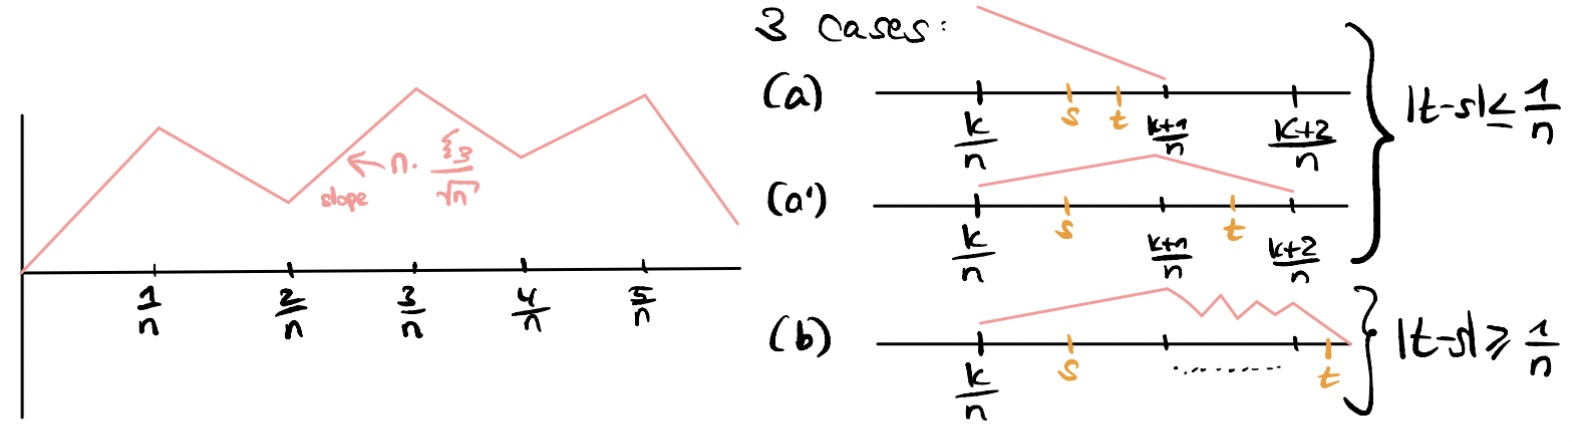
\includegraphics[scale=0.2]{Donsker.jpeg}
				\end{center}
			\end{figure}
			If $|t-s|<\frac{1}{n}$ there are two simple cases to be distinguised (either there is a bend between $t$ and $s$ or there isn't), for $|t-s|\geq \frac{1}{n}$ we argue differently. Let us start with small $|t-s|$:
			\begin{itemize}
				\item[(a)] If $|t-s|<\frac{1}{n}$ and there is no bend between $s$ and $t$, say $\frac{k}{n}<s<t<\frac{k+1}{n}$, then
    			\begin{align*}
    				\lvert X_t^n - X_s^n \rvert^4 = \lvert (t - s)\cdot \text{slope} \rvert^4 = \lvert t - s\rvert^4 \cdot n^4 \cdot \frac{Y_{k+1}^4}{n^2} \leq \lvert t - s \rvert^2\cdot  Y_{k+1}^4.
				\end{align*}
				\item[(a')] If $|t-s|<\frac{1}{n}$ and there is a bend between $s$ and $t$, say $s<\frac{k+1}{n}<t<\frac{k+2}{n}$, then
				\begin{align*}
					\lvert X_t^n - X_s^n \rvert 
					\overset{\Delta}&{\leq} \big|X_t^n-X^n_{\frac{k+1}{n}}\big|+\big|X^n_{\frac{k+1}{n}}-X_s^n\big|\\					
						&\leq \lvert t -s \rvert \cdot n \cdot \frac{\lvert Y_{k+2}\rvert}{\sqrt{n}} + \lvert t -s \rvert \cdot n \cdot \frac{\lvert Y_{k+1}\rvert}{\sqrt{n}} \\
						&= \lvert t -s \rvert \sqrt{n} \left( \lvert Y_{k+2}\rvert + \lvert Y_{k+1}\rvert\right)\\
						&= \lvert t -s \rvert^{1/2} \left( \lvert Y_{k+2}\rvert + \lvert Y_{k+1}\rvert\right).
				\end{align*}
				%so that $\lvert X_t^n - X_s^n \rvert^4 \overset{\lvert t-s \rvert \leq \frac{1}{n}}{\leq} \lvert t-s \rvert^2 \left( \lvert Y_{k+1}\rvert + \lvert Y_{k+2}\rvert\right)^4$.
			\end{itemize}
			Combining both cases yields
			\begin{align*}
				\E[|X_t-X_s|^4]\leq c|t-s|^2,\quad \text{with } c=\max\big\{\E[Y_1^4], \E[(|Y_1|+|Y_2|)^4]\big\},
			\end{align*}
			for all $t,s$ with $|t-s|<\frac{1}{n}$.	
			%Let us first check the differences on points where the interpolation is irrelevant, that is $\{ \frac{k}{n}\colon n\in \N\}$:
			%\begin{align*}
			%	X_{\frac{k}{n}}^n - X_{\frac{l}{n}}^n = \sum_{i=1}^{k}\frac{Y_i}{\sqrt{n}} - \sum_{i=1}^{l} \frac{Y_i}{\sqrt{n}} = \sum_{j=l+1}^k \frac{Y_j}{\sqrt{n}}
			%\end{align*}
			%and we know how to estimate $\E\left[ \lvert X_t - X_s \rvert^4\right]$ as in the proof of the strong law of large numbers with $4$th moments (compare the proof of Theorem \ref{sGGZ}). 
			For $|t-s|\geq \frac{1}{n}$ we will work with the explicite difference
			\begin{align}\label{yellow_box}
				\begin{split}
				X_t^n - X_s^n 
				&= \sum_{j=\lfloor ns \rfloor +1 }^{\lfloor nt \rfloor} \frac{Y_j}{\sqrt{n}}+\left( nt - \lfloor nt \rfloor\right) \frac{Y_{\lfloor nt \rfloor +1 }}{\sqrt{n}} -\left( ns - \lfloor ns \rfloor\right) \frac{Y_{\lfloor ns \rfloor + 1}}{\sqrt{n}}\\
				&= \sum_{j=\lfloor ns \rfloor +2 }^{\lfloor nt \rfloor} \frac{Y_j}{\sqrt{n}}+\left( nt - \lfloor nt \rfloor\right) \frac{Y_{\lfloor nt \rfloor +1 }}{\sqrt{n}} +(1-(ns - \lfloor ns \rfloor)) \frac{Y_{\lfloor ns \rfloor + 1}}{\sqrt{n}}.
				\end{split}
			\end{align}
			Before estimating two tricks are needed. The first trick uses an idea from the first proof of the strong law of large numbers (compare the proof of Theorem \ref{sGGZ}), the fourth moment computation for centered independent random variables:
			\begin{align}\label{red_star}
				\E \Big[ \Big( \sum_{j=1}^N Y_j\Big)^4\Big] &= \E \Big[ \sum_{i,j,l,n=1}^N Y_i \cdot Y_j \cdot Y_l \cdot Y_n\Big] 
				 \overset{\text{iid and }\E[Y_i]=0}= N  \E[Y_1^4] + \frac{N(N-1)}{2} (\E[Y_1^2])^2.
			\end{align}
			The equalities hold as all products vanish that have a single of the $Y$ factors, only the ones remain that have a fourth power or two second powers. The second little trick needed is to estimate, for independent and centered $X$,$Y$ and $a\in [-1,1]$, 
			\begin{align}\label{last}
				\begin{split}
				\E\big[ \left(aX+Y\right)^4\big] &= a^4 \E\big[X^4\big] + 6 a^2 \E\big[X^2\big]\E\big[Y^2\big] + \E\big[Y^4\big] \\
					&\leq \E\big[X^4\big] + 6 \E\big[X^2\big]\E\big[Y^2\big] + \E\big[Y^4\big] = \E\big[ (X+Y)^4\big].
			\end{split}
			\end{align}
			The second trick will be applied twice to the righthand side of \eqref{yellow_box}, first with $a=nt - \lfloor nt \rfloor$ and to the remaining sum with $a=1-(ns - \lfloor ns \rfloor)$.
			\begin{itemize}
				\item[(b)] If $|t-s|\geq \frac{1}{n}$, then the above yields
					\begin{align*}
						\E \left[ \lvert X^n_t - X^n_s \rvert^4 \right]
						\overset{\eqref{last}}&{\leq} \E\Big[\Big(\sum_{j=\lfloor ns \rfloor +2 }^{\lfloor nt \rfloor+1} \frac{Y_j}{\sqrt{n}}+(1-(ns - \lfloor ns \rfloor)) \frac{Y_{\lfloor ns \rfloor + 1}}{\sqrt{n}}\Big)^4\Big]\\
						\overset{\eqref{last}}&{\leq} \frac{1}{n^2} \E\Big[ \Big( \sum_{j=\lfloor ns \rfloor +1}^{\lfloor nt \rfloor + 1}Y_j \Big)^4\Big] \\
						\overset{\text{iid}}&{=} \frac{1}{n^2} \E\Big[ \Big( \sum_{j=1}^{\lfloor nt \rfloor -\lfloor ns \rfloor +1}Y_j \Big)^4\Big] \\
							\overset{\eqref{red_star}}&{\leq} \frac{\left(\lfloor nt\rfloor - \lfloor ns \rfloor+1\right)\cdot \E[Y_1^4]+\left( \lfloor nt \rfloor - \lfloor ns \rfloor+1\right)^2 
							\cdot 1}{n^2} \\
							&\leq \frac{ 3 \lvert t-s \rvert \cdot n\cdot  \E[Y_1^4]+ 9 \lvert t-s \rvert^2 \cdot n^2 \cdot \sigma^2}{n^2} \\
							&\leq \big( 3 \E[Y_1^4]+9\big)\cdot \lvert t-s \rvert^2,
					\end{align*}
					where we also used that, for $|t-s|\geq \frac{1}{n}$,
					\begin{align*}
						\lfloor nt\rfloor - \lfloor ns \rfloor+1\leq nt-(ns-1)+1=n(t-s)+1+1\leq 3n(t-s).
					\end{align*}
			\end{itemize}
			Combining the cases (a), (a'), and (b) yields
			\begin{align*}
					\E\left[ \lvert X^n_t - X^n_s \rvert^4\right]\leq C \cdot \lvert t-s \rvert^2,
				\end{align*}
			for all $t,s\geq 0$, with a constant $C \coloneqq \max \{ \E[Y_1^4], \E[(|Y_1|+|Y_2|)^4],( 3\E[Y_1]+9)\}$ that is independent of $n$.
\end{proof}
Kolmogorov's tightness criterion essentially tells us that scaled random walks (with 4th moments) stay (with high probability) almost $\frac{1}{4}$-H\"older continuous when the scaling factor is increased. This is clearly related to finiteness of moments as big jumps produce rough spikes in a linearly interpolated random walk (see the drawing).
\begin{figure}[h]
	\begin{center}
		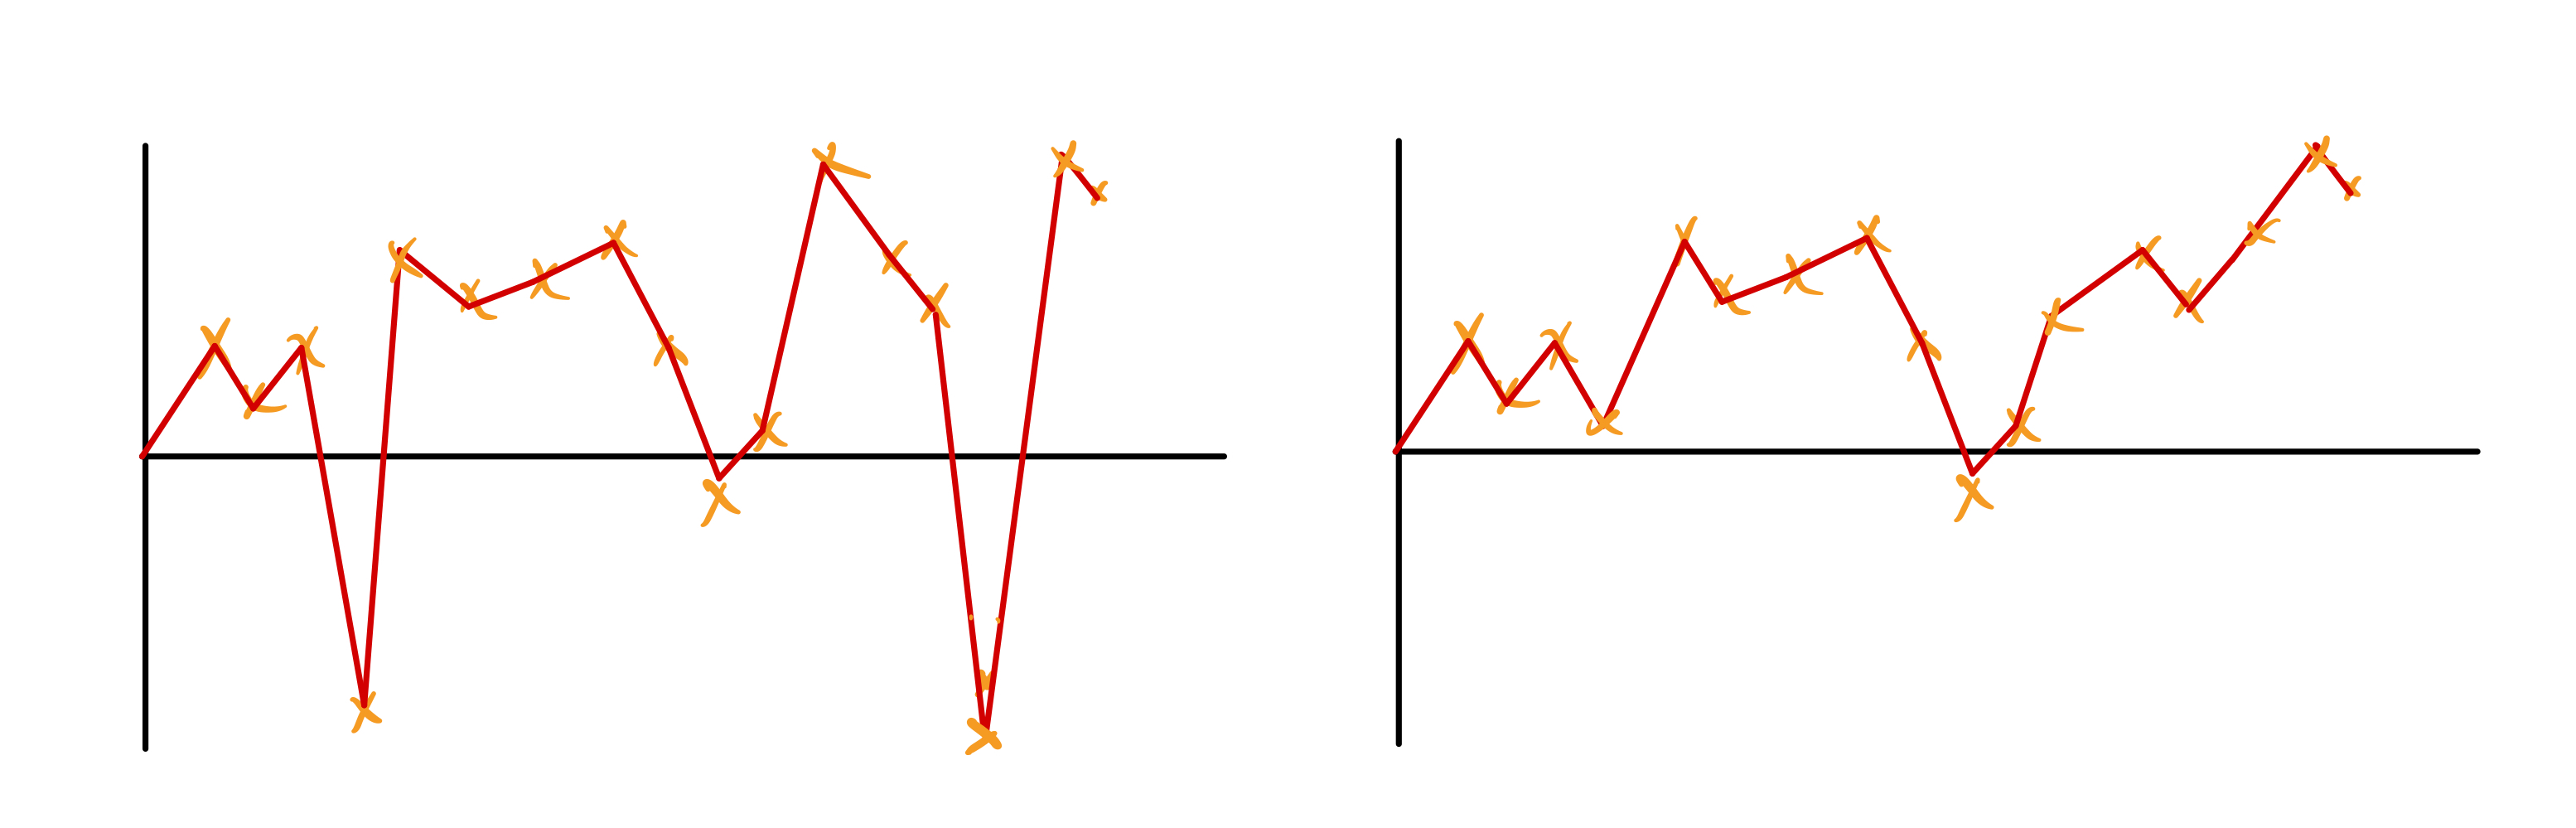
\includegraphics[scale=0.1]{spikes.jpeg}
		\caption*{Big jumps, sharp spikes, rough paths - small jumps, less rough}
	\end{center}
\end{figure}
With a bit more work one can check a refined Kolmogorov-Chentsov condition showing that the scaled random walks are uniformly in $n$ almost $\frac{1}{2}$-H\"older continuous. This is exactly the amount of rougness that the scaled process must achieve in the limit to be a Brownian motion. If $\E[Y_1^2]=\infty$, then the central limit theorem and Donsker's theorem fail! The roughness increases more and more, ripping apart the sample paths in the limit. Replacing the scaling $n^{\frac{1}{2}}$ by $n^{\frac{1}{\alpha}}$ for the right choice of $\alpha$ leads to stable distributions and $\alpha$-stable L\'evy processes. Those processes bear a lot of similarity with the Brownian motion but have discontinuous paths. They share the L\'evy property for increments, satisfy the scaling property (with $\alpha$ instead of $2$), and their one-dimensional distributions $X_t$ have a similar characteristic function (compare Example \ref{example:stable}). The scaling parameter $\alpha$ is essentially the smallest number with $\E[|Y_1|^\alpha]=\infty$. The magic is that for different $\alpha$ the limiting processes look different (few massive jumps dominate for $\alpha \approx 0$, paths look more like Brownian paths for $\alpha\approx 2$) but for finite second moments scaling limits of random walks are \underline{always} the Brownian motion no matter how many further moments are exist.\smallskip


We have already discussed the difference between weak convergence and fdd convergence, weak convergence immediately implies convergence in distribution of the random variables $(F(X^n))_{n\in\N}$ towards $F(X)$ for \underline{all} continuous functionals $F:C([0,\infty))\to \R$. It is not always possible to prove the tightness but if so this is \underline{much} more interesting than only convergence of $(X^n_{t_1},...,X^n_{t_k})$ towards $(X_{t_1},...,X_{t_k})$. As an example let us deduce from Donsker's theorem a statement on random walks $X$ with jump-sizes $Y_1,Y_2,...$ by using the continuous functional $F(g)=\sup_{t\in [0,1]}|g(t)|$:
\begin{laufmerksamkeit}
	Erd\"os and Kac in 1946 computed a couple of probabilities for random walks. While the central limit theorem implies that a centered random walk with second moment $(\E[Y_1]=0$ and $\sigma^2=\Var[X_1]<\infty)$ at time $n$ is roughly distributed according to $\mathcal N(0,\sigma^2 n)$, the distribution of the running supremum $X^*_n:=\max_{k\leq n}|X_k|$ is more complicated to obtain. It certainly holds that $X^*_n\geq X_n$ but how much larger? Erd\"os and Kac proved that 
	\begin{align*}
		\lim_{n\to\infty}\P\big(X^*_n\leq \alpha \sqrt{n}\big)= \begin{cases}
			0&:\alpha \leq 0\\
			\sqrt{\frac{2}{\pi}}\int_0^\alpha e^{-\frac{x^2}{2\sigma^2}}\dint x&: \alpha>0
		\end{cases},
	\end{align*}
	so the running supremum is roughly distributed as $|Z|$ for $Z\sim \mathcal N(0,1)$. 
	The original proofs were mostly by hands, Donsker, as a corollary of his theorem, gave the following proof. Chosing $F(g)=\sup_{t\in [0,1]}|g(t)|$, Theorem \ref{thm:donsker} implies 
	\begin{align*}
		\frac{1}{\sigma \sqrt{n}} X^*_n=\frac{1}{\sigma \sqrt{n}}\sup_{t\in [0,1]} |X_t^n| \overset{(d)}{\rightarrow} \sup_{t\in [0,1]}|B_t|,\quad n\to\infty.
	\end{align*}
	The righthand side is known to have the same distribution as $|B_1|$ by the so-called reflection principle of the Brownian motion, hence, the claim follows.
\end{laufmerksamkeit}
Donsker's theorem is the first step into the big world of probability research. During the past decades different objects have been identified that arise as universal scaling limits of different discrete stochastic objects. They all have in common that they relate to the Brownian motion or the stable processes. Just to mention two further examples, the continuum random trees are scaling limits of discrete random trees such as the ones appearing in the branching process of Example \ref{GW}. The Brownian map is the universal scaling limit of many different random maps (think of randomly created maps of contries on a continent) such as triangulation (every country has precisely three neighhboring countries). Here are two realisations of the Brownian continuum random tree and the Brownian map 
\footnote{Check the websites of \href{https://igor-kortchemski.perso.math.cnrs.fr/images.html}{Igor Kortchmenski} and \href{http://www.normalesup.org/~bettinel/simul.html}{J\'er\'emy Bettinelli} for more simulations.}.
\begin{figure}[h]
	\begin{center}
		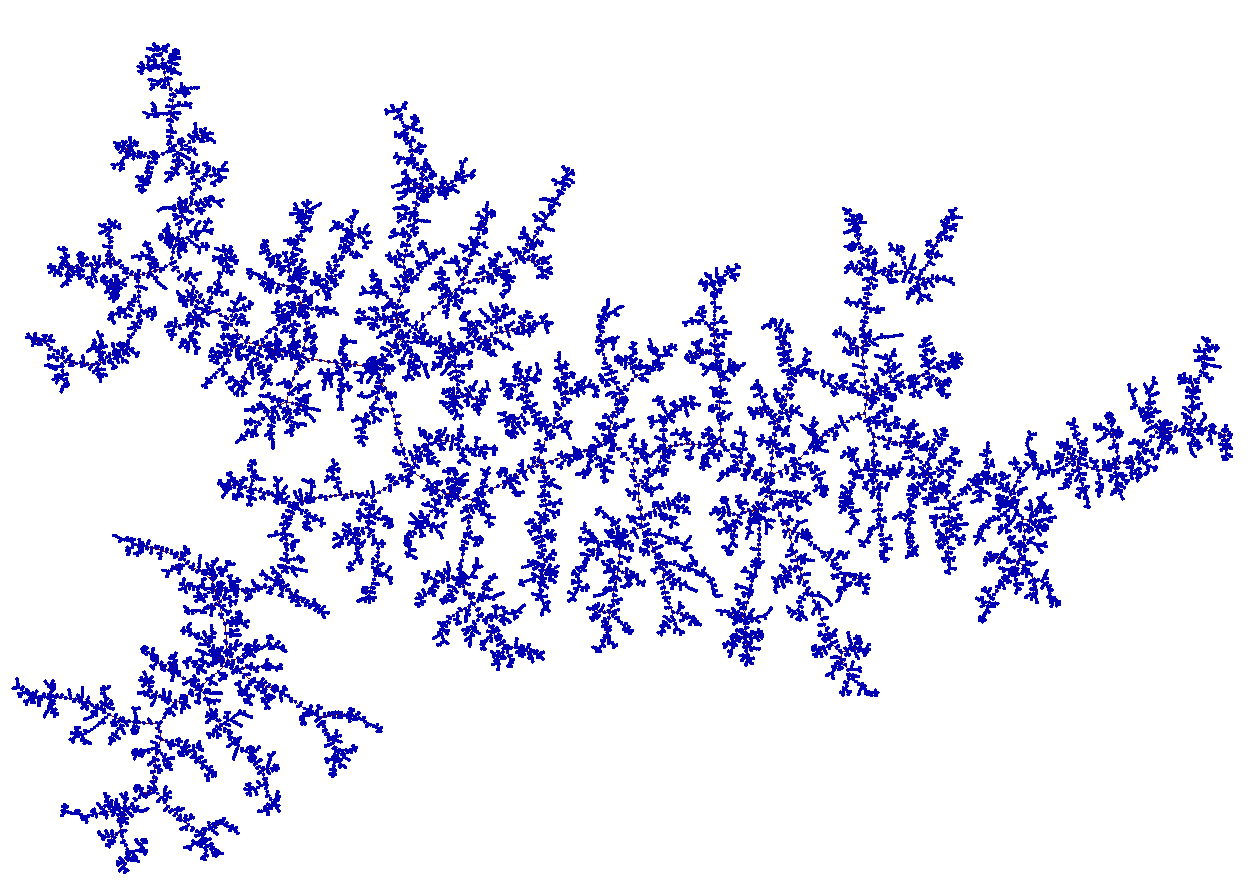
\includegraphics[scale=0.3]{CRT.jpg}
		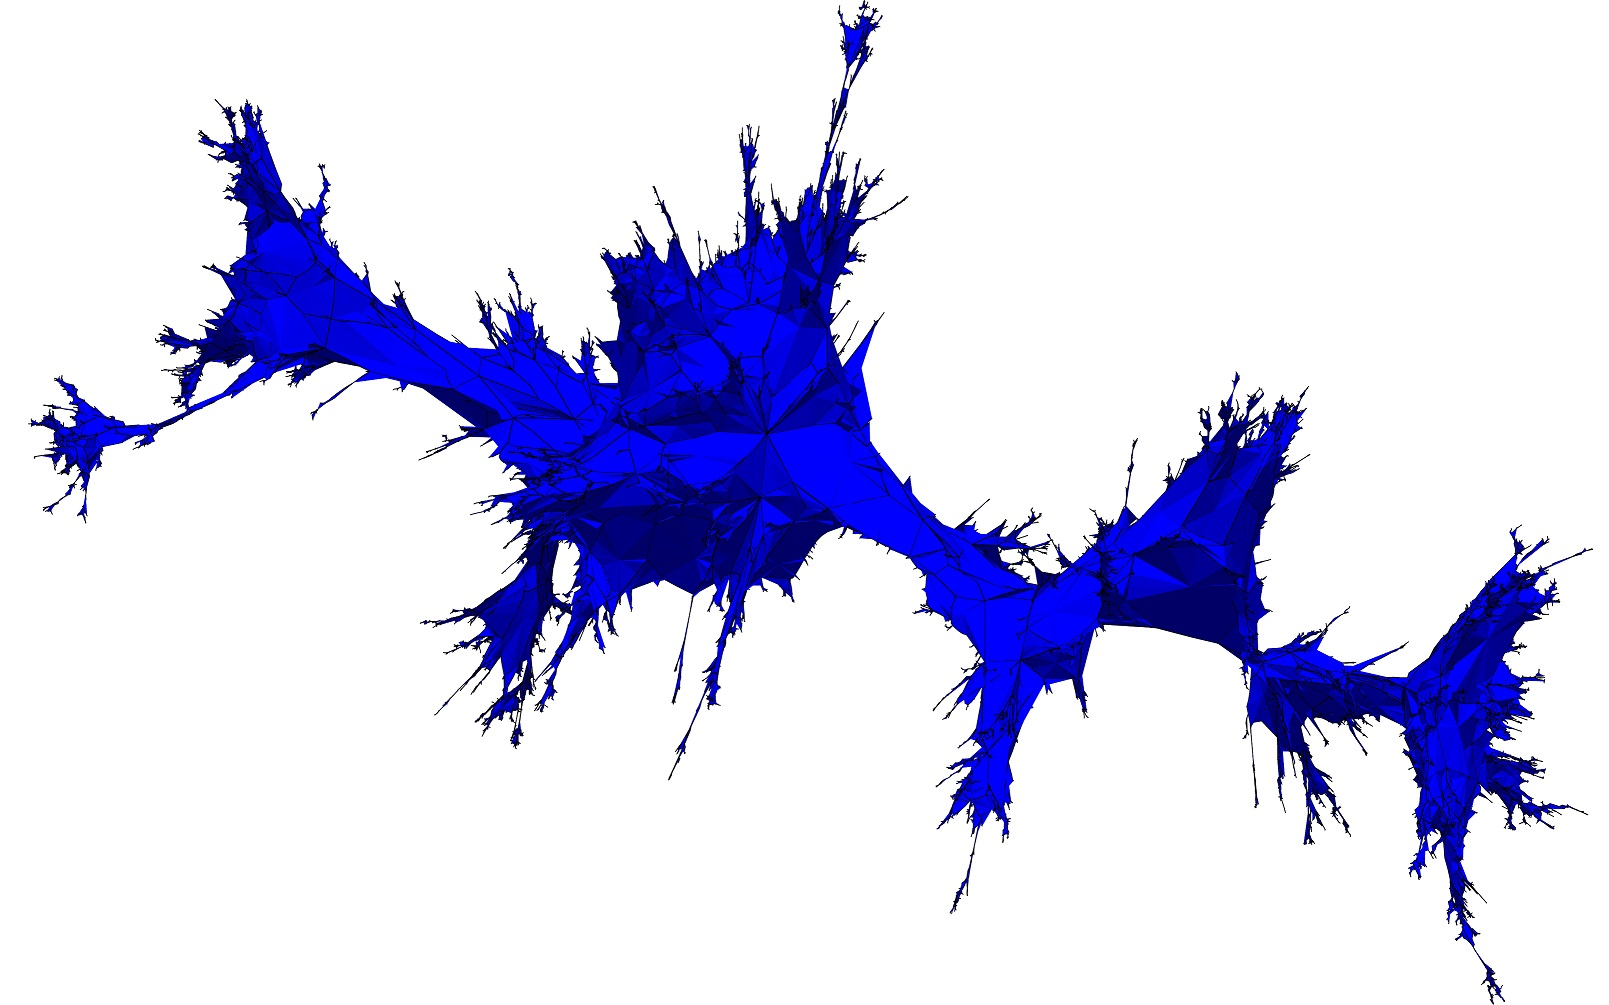
\includegraphics[scale=1.7]{BrownianMap.jpg}
		\caption*{Realisations of the continuum random tree and the Brownian map}
	\end{center}
\end{figure}

